\documentclass[11pt, twoside,openright]{article}
\usepackage[utf8]{inputenc}
\usepackage[T1]{fontenc}     % Recommended for better font encoding
\usepackage{csquotes}        % Recommended for biblatex
\setcounter{secnumdepth}{3}
\usepackage{setspace}
\usepackage{sectsty}
\usepackage{fullwidth}
\usepackage{placeins}
\usepackage{subcaption}

\usepackage[paperwidth=8.5in,paperheight=14.2885in]{geometry}
\geometry{left=2.54cm, right=2.54cm, top=3.81cm, bottom=3.81cm}
% Include the listings package for syntax highlighting of code

\usepackage[]{listingsutf8}
\usepackage[dvipsnames]{xcolor} 
\usepackage{amssymb,amsmath} 
\usepackage{dutchcal}
\usepackage{textcomp}

\usepackage{pdfpages}
\usepackage{qlanth} 
\usepackage{scalerel}
\usepackage{changepage}
\usepackage{xparse}

\usepackage{mdframed}
\usepackage{pgffor}
\usepackage{titlesec}

\graphicspath{{figures/}}
\usetikzlibrary{decorations.pathmorphing}
\usepackage{lmodern}
\usepackage{etoolbox} % for patching commands
\usepackage[htt]{hyphenat} %Enable hythenation of TT text:

\usepackage[backend=bibtex,style=alphabetic,doi=false,url=false]{biblatex}
\addbibresource{qlanth.bib} 

\allsectionsfont{\centering}

\usepackage[para]{footmisc}
\usepackage{etoolbox}
\robustify{\underbar}

% Listing configuration
\lstset{   
    language=Mathematica,
    inputencoding=utf8,         % Set your language (you can change the language for each code-block optionally)
    basicstyle=\ttfamily\color{darkgray}\footnotesize,       % The size of the fonts that are used for the code
    literate=
        {\\[Alpha]}{{$\alpha$}}{1}
        {\\[Beta]}{{$\beta$}}{1}
        {\\[Gamma]}{{$\gamma$}}{1}
        {\\[Zeta]}{{$\zeta$}}{1}
        {\\[VerticalSeparator]}{|}{1}
        {é}{{\'e}}{1}
        ,  
    keywordstyle=\color{blue},        % Keyword style
    stringstyle=\color{OliveGreen},        % String literal style
    commentstyle=\color{cyan},        % Comment style
    morecomment=[l][\color{magenta}]{\#},
    breakatwhitespace=false,          % Sets if automatic breaks should only happen at whitespace
    breaklines=true,                  % Sets automatic line breaking
    captionpos=b,                     % Sets the caption-position to bottom
    keepspaces=true,                  % Keeps spaces in text, useful for keeping indentation of code (possibly needs columns=flexible)
    showspaces=false,                 % Show spaces everywhere adding particular underscores; it overrides 'showstringspaces'
    showstringspaces=false,           % Underline spaces within strings only
    showtabs=false,                   % Show tabs within strings adding particular underscores
    tabsize=2,                        % Sets default tabsize to 2 spaces
    frame=single,                     % Adds a frame around the code
    numbers=left,                     % Where to put the line-numbers; possible values are (none, left, right)
    numberstyle=\tiny\color{gray},    % Style used for line-numbers
    stepnumber=1,                     % Step between two line-numbers. If it's 1, each line will be numbered
    numbersep=5pt,                    % How far the line-numbers are from the code
    xleftmargin=0.8cm,                % Margin from left
    xrightmargin=0.3cm              % Margin from right
}
\usepackage[colorlinks=true,
			citecolor=blue,
			linkcolor=blue,
			urlcolor=cyan,
			bookmarks=true,
			bookmarksnumbered=true
			]{hyperref}
\usepackage{makeidx}
\makeindex

\DeclareUnicodeCharacter{2212}{\ensuremath{-}}

\usepackage{fancyhdr}
\pagestyle{fancy}
\fancyhf{}
\renewcommand{\headrulewidth}{0pt} % Optional: Removes the header rule
\cfoot{\hyperref[toc]{\thepage}}

\fancypagestyle{plain}{
    \fancyhf{}  % Clear all header and footer fields
    \fancyfoot[C]{\hyperref[toc]{\thepage}}  % Center footer
    \renewcommand{\headrulewidth}{0pt}  % Remove header rule
    \renewcommand{\footrulewidth}{0pt}  % Remove footer rule
}

\titleformat{\chapter}[display]
  {\normalfont\Huge\bfseries\centering} % Format for chapter title
  {\chaptername\ \thechapter} % Format for "Chapter #" part
  {-10pt} % Space between "Chapter #" and the chapter title
  {\huge} % Format for the chapter title

\titlespacing*{\chapter}{0pt}{-10pt}{20pt} % Adjust spacing

\begin{document} 

\begin{titlepage} % Start of the title page
    \centering
    \vspace*{\fill}
    
    % Include the image
    {\Large\qlanth}\\
    {\large doc version $\ket{\alpha}^{(17)}$} \\
    \vspace*{0.5cm}
    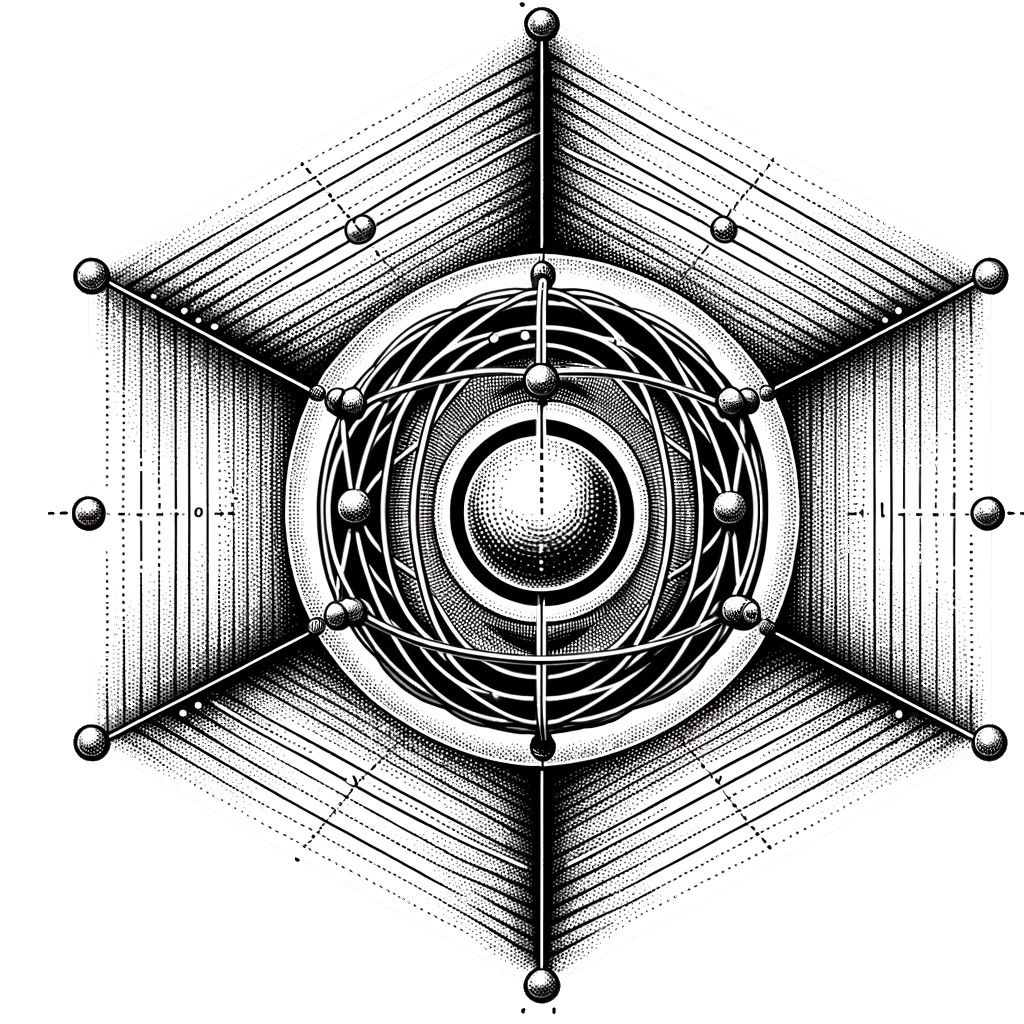
\includegraphics[width=0.6\textwidth]{ion_in_lattice.jpg}  % Adjust the size as needed
    \vspace*{0.4cm} % More vertical space a
    
    % Additional information
    {\large Juan David Lizarazo Ferro,}\\
    {\large Christopher Dodson}\\
    {\large \& Rashid Zia}\\
    
	\vspace*{\fill}
\end{titlepage}

\newpage

\thispagestyle{empty}
\vspace*{\fill}
\begin{center}
$\,$ \\
{\large Brown University, \\ Department of Physics}\\
\vspace{0.2cm}
\hrulefill \\
\vspace{0.2cm}
Providence, Rhode Island \\
\codetext{2025 AD}
\end{center}

\newpage

\thispagestyle{empty}

\vspace*{\fill}

\begin{center}
\qlanth may be downloaded

\href{https://github.com/zia-lab/qlanth}{here}
\vspace{-0.4cm}
\begin{figure}[h!]
	\begin{center}
		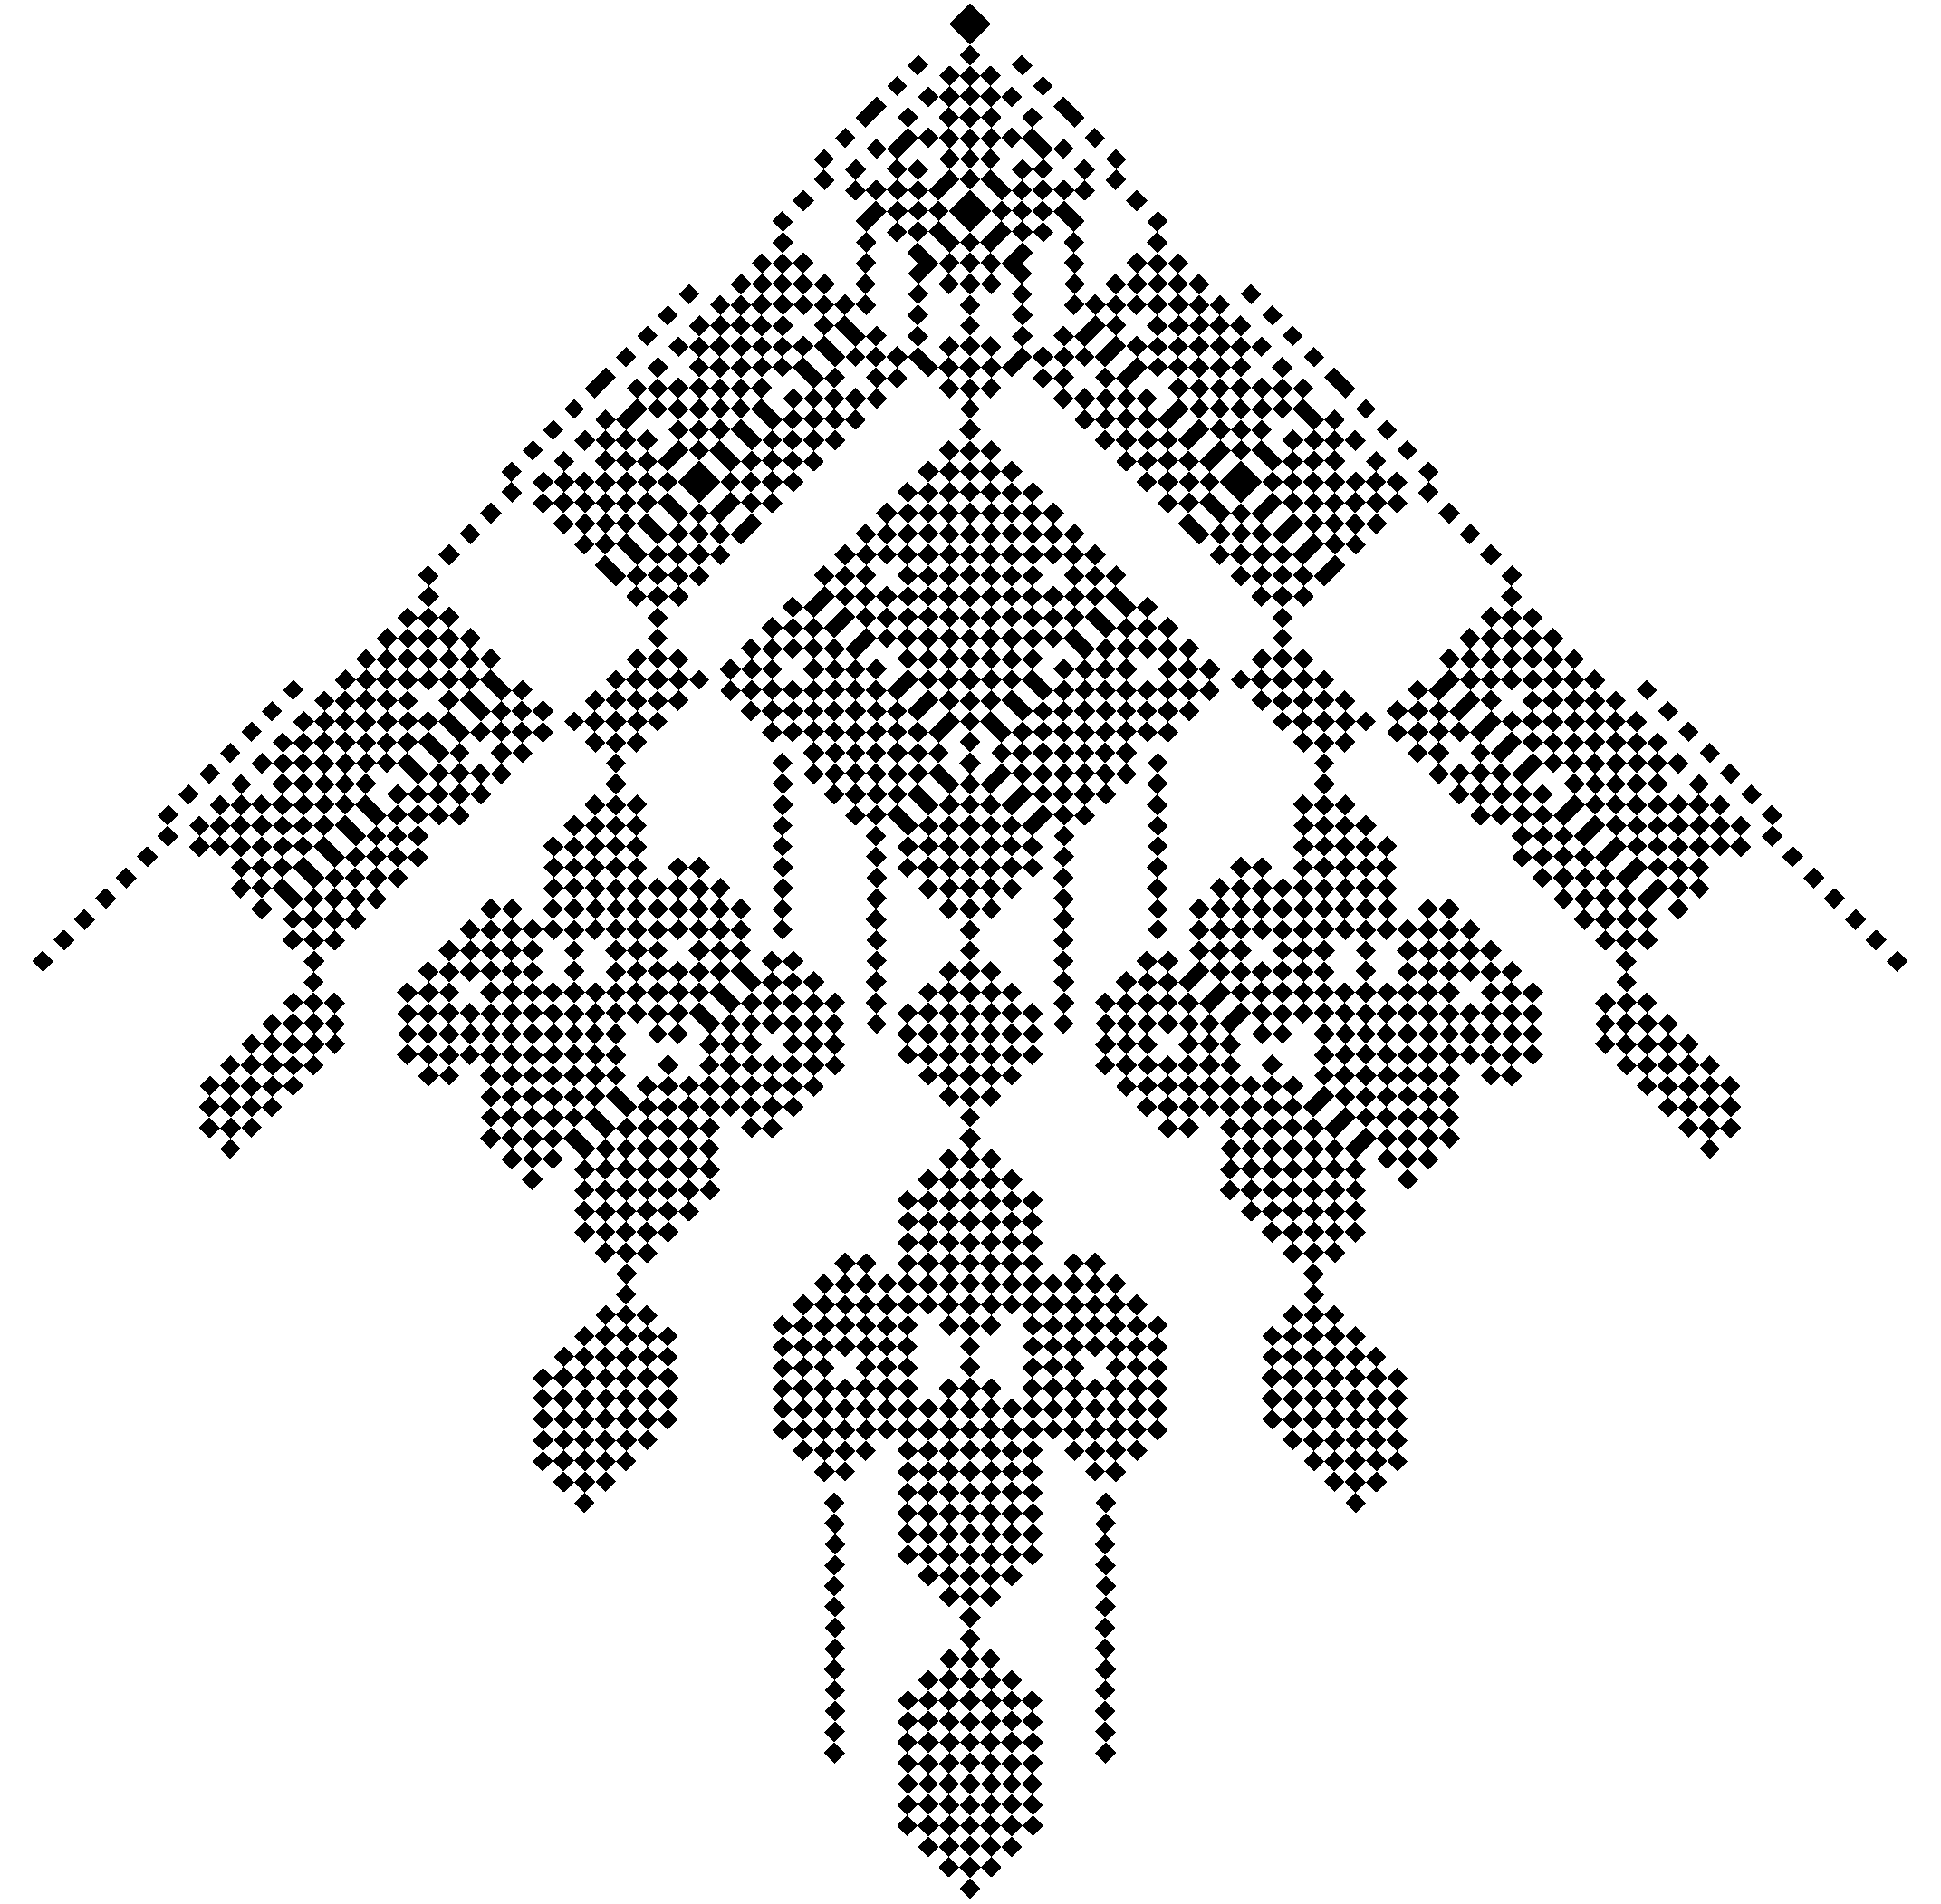
\includegraphics[width=0.95\textwidth]{./figures/pr_code.png}
	\end{center}
\end{figure}
\end{center}

\vspace*{\fill}

\cleardoublepage

\thispagestyle{empty}

\vspace*{\fill}

\begin{center}
\vspace{-0.27cm}
\begin{figure}[h!]
	\begin{center}
		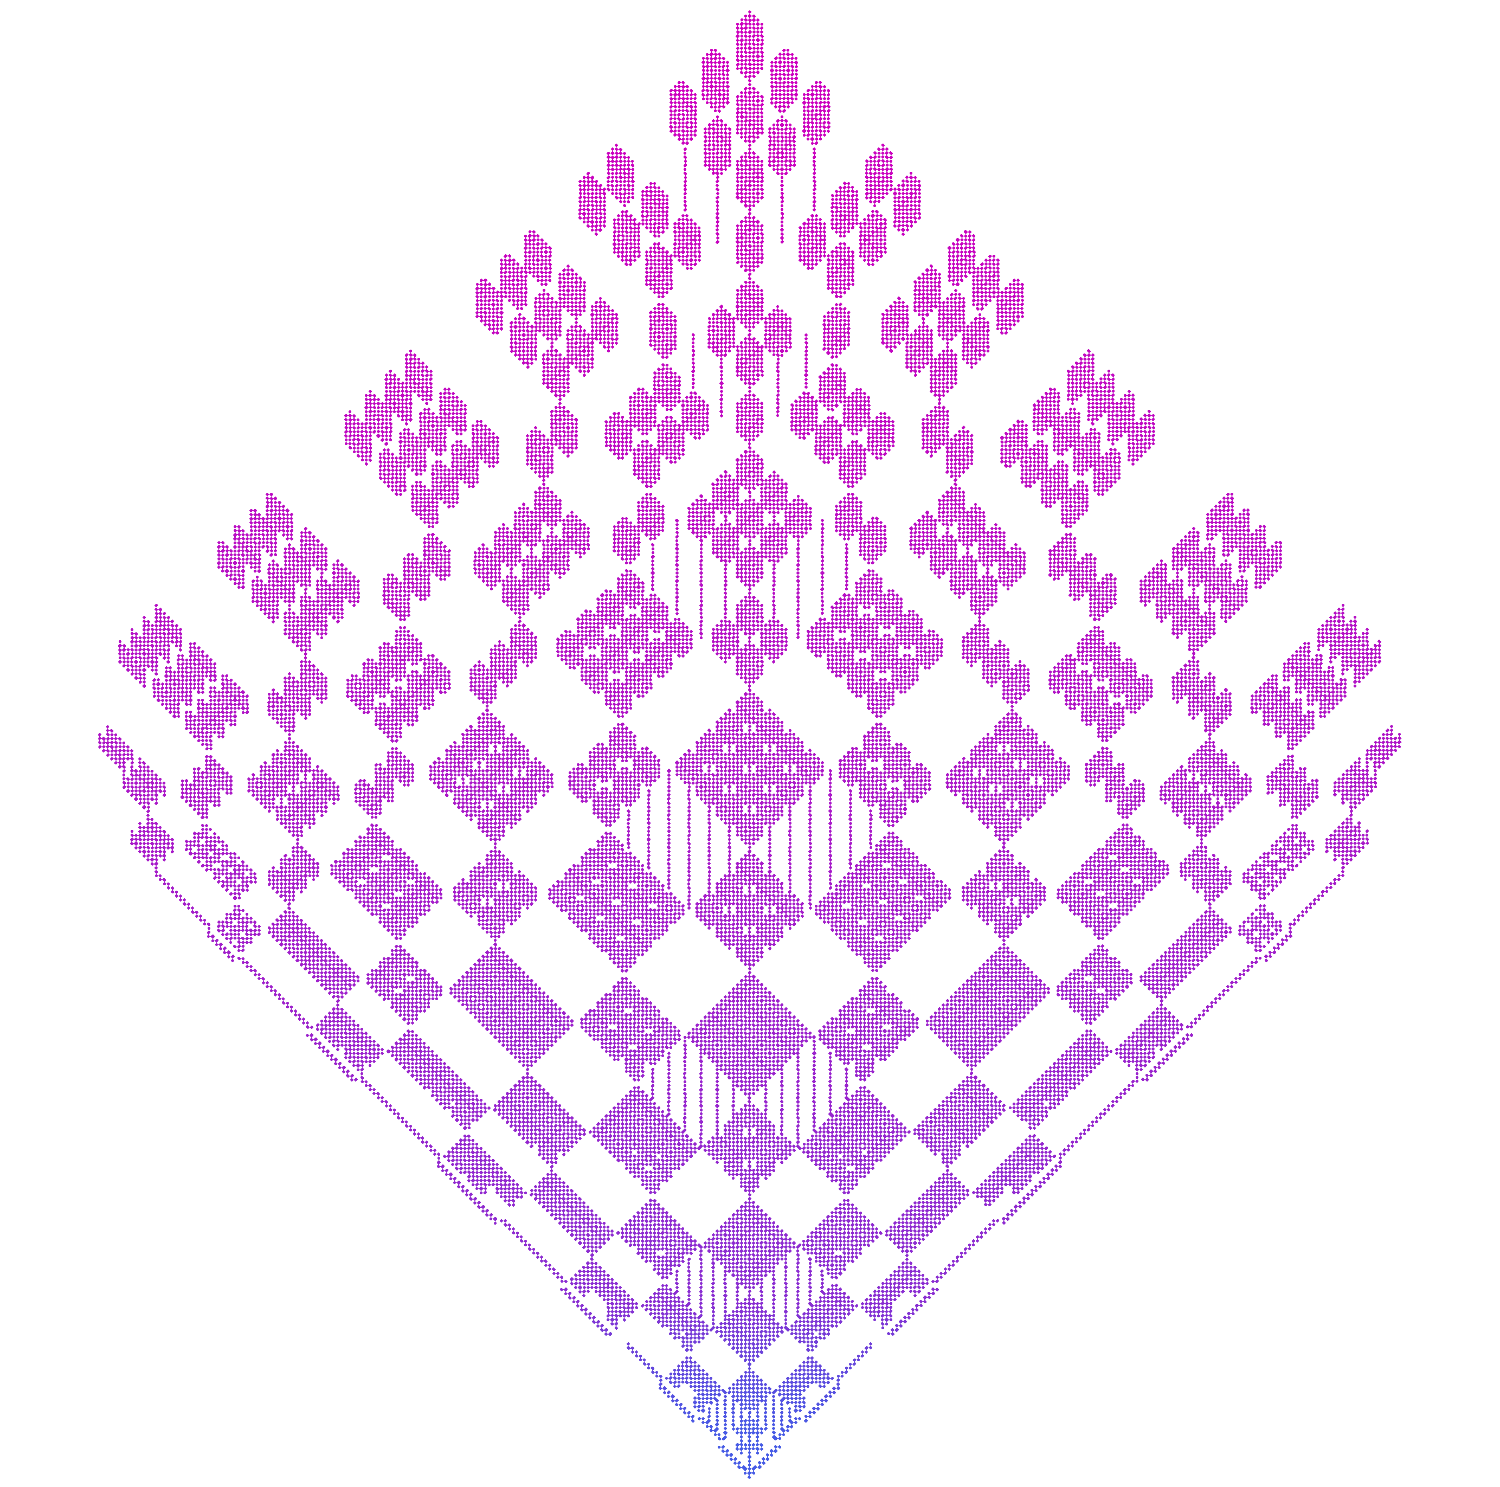
\includegraphics[width=0.95\textwidth]{nd_code.png}
	\end{center}
\end{figure}
\vspace{-0.7cm}
This work was sponsored by the \\ \textbf{National Science Foundation} \\ Grant No. \codetext{DMR-1922025}
\end{center}


\vspace*{\fill}

\cleardoublepage

\pagenumbering{roman}

\vspace*{\fill}

\qlanth is a tool that can be used to estimate the electronic structure of lanthanide ions in crystals. I uses an effective Hamiltonian limited to a single-configuration with included configuration-interaction corrections. This Hamiltonian aims to describe the observed properties of ions embedded in solids in a picture that imagines them as free-ions modified by the influence of the lattice in which they find themselves in.

This picture of lanthanide ions is one that developed and mostly matured in the second half of the last century by the efforts of 
John Slater,\footnote{\cite{slater_theory_1929}}
Giulio Racah,\footnote{\cite{racah_theory_1942-1,racah_theory_1942,racah_theory_1943,racah_theory_1949}}
Brian Judd,\footnote{\cite{judd_optical_1962,judd_operator_1963,judd_configuration_1963,judd_three-particle_1966,judd_second_1967,judd_intra-atomic_1968,crosswhite_magnetic_1968,judd_parametric_1982,judd_operator_1983,judd_complete_1984,judd_orthogonalized_1984,judd_complex_1985,judd_classification_1986,judd_atomic_1988,judd_developments_1989,judd_symmetries_1993,judd_group_1996,judd_interaction_2005}}
Gerhard Dieke,\footnote{\cite{dieke_spectra_1963,piksis_energy_1967,dieke_spectra_1968}}
Hannah Crosswhite,\footnote{\cite{crosswhite_magnetic_1968,crosswhite_effective_1971,crosswhite_spectrum_1976,crosswhite_parametric_1977,dieke_spectra_1963,judd_intra-atomic_1968,judd_orthogonalized_1984}}
Robert Cowan,\footnote{\cite{cowan_theory_1981}}
Michael Reid,\footnote{\cite{reid_applications_1981}}
William Carnall,\footnote{\cite{carnall_spectral_1965,carnall_systematic_1989,carnall_systematic_1992,carnall_electronic_1968-1,carnall_spectral_1968,carnall_electronic_1968-2,carnall_electronic_1968-3,carnall_electronic_1968,carnall_absorption_1970,carnall_energy_1976,gorller-walrand_magnetic_1991}}
Clyde Morrison,\footnote{\cite{morrison_crystal-field_1976,morrison_crystal-field_1979,morrison_energy_1994,morrison_host_1980,morrison_analysis_1987,morrison_theoretical_1977,morrison_rare-earth_1977,morrison_spectroscopic_1982,morrison_optical_1983}}
Richard Leavitt,\footnote{\cite{leavitt_complete_1987,leavitt_role_1982,leavitt_crystal-field_1980,morrison_crystal-field_1979,morrison_spectroscopic_1982}}
Brian Wybourne,\footnote{\cite{carnall_spectral_1965,conway_low-lying_1963,rajnak_configuration_1963,rajnak_electrostatically_1964,rajnak_configuration_1964,wybourne_low-lying_1964,wybourne_orbitorbit_1964,wybourne_spectroscopic_1965,wybourne_symmetry_1970,wybourne_optical_2007}}
Richard Trees,\footnote{\cite{trees_l_1952,trees_spin-spin_1951,trees_comparison_1958}}
and Katherine Rajnak\footnote{\cite{rajnak_configuration_1963,rajnak_electrostatically_1964,rajnak_configuration_1964,rajnak_configuration_1965}} among others. The goal of this tool is to provide a modern implementation of the methods that resulted from their work. This code is written in Wolfram language.

Separate to their specific use in this code, \qlanth also includes data that might be of use to those interested in the single-configuration description of lanthanide ions. These data include the \cfps (as calculated by Velkov and parsed here), and reduced matrix elements for all the operators in the effective Hamiltonian. These are provided as standard \mathematica associations that should be simple to use elsewhere. One feature of \qlanth is that symbolic expressions are maintained up to the very last moment where numerical approximations are inevitable. As such, the symbolic expressions that result for the matrix representation of the Hamiltonian, result in linear combinations of the model parameters with symbolic coefficients.

The included \mathematica notebook \codetext{qlanth.nb} lists most of the functions included in \qlanth and should be considered complementary to this document. The \codetext{/examples} folder includes notebooks containing the result of this description for most of the trivalent lanthanide ions in lanthanum fluoride. \LaFthree is remarkable in that it was one of the systems in which a systematic study \cite{carnall_systematic_1989} of all of the trivalent lanthanide ions were studied.

This code was originally authored by Christopher Dodson and Rashid Zia for their research into magnetic dipole transitions in lanthanide ions \cite{dodson_magnetic_2012}. Here it has been rewritten and expanded by David Lizarazo. It has also benefited from conversations with Tharnier Puel at the University of Iowa.

This document has \ref{section:code} sections. \sectionref{section:the-semi-hamiltonian} gives an overview the \hamilton. \sectionref{section:ls-basis} explains the details of the basis in which the \hamilton is evaluated, together with the method of fractional parentage, additional quantum numbers, Kramer's degeneracy, and the JJ' block structure of the \hamilton. \sectionref{section:interactions} gives a detailed explanation of each of the interactions include in the \hamilton. \sectionref{section:coord-sys} gives explains the implicit assumptions in the orientation of the coordinate system. \sectionref{section:uncertainty} gives an overview of the attendant experimental setups and considerations about uncertainty. \sectionref{section:transitions} is about the calculation of magnetic and forced electric dipole transitions.  \sectionref{section:param-constraints} explain certain constraints often used for the parameters in the \hamilton.
 
\sectionref{section:data-fitting} explains the details of fitting the Hamiltonian to experimental data.\sectionref{section:notebooks} lists included auxiliary \mathematica notebooks. \sectionref{section:sparsefn} explains the details of an abbreviated Python extension to \qlanth. \sectionref{section:data-sources} explains some of the included experimental data.  \sectionref{section:other-details} contains a few assorted details on running \qlanth. \sectionref{section:units} has a brief comment on units. \sectionref{section:notation} and \sectionref{section:definitions} include a summary of notation and definitions used throughout this document. Finally, \sectionref{section:code} contains a printout of the code included in \qlanth.

Besides being a fully functional code that works out of the box, \qlanth is unique in that it also includes computational routines that can generate from scratch (or close to scratch) the necessary reduced matrix elements which in other codes are simply loaded from other vintages. Great care was taken to comment every loop, variable, procedure, and data provenance. To highlight this, the code relevant to the different functions has been interspersed in the parts where they are mentioned.

\vspace*{\fill}

\newpage

\hypertarget{toc}{}

\vspace*{\fill}

\tableofcontents \label{toc}

\vspace*{\fill}

\newpage

\pagenumbering{arabic}

\section{The \hamilton}\label{section:the-semi-hamiltonian}

Electrons in a multi-electron ion are subject to a number of interactions. They are attracted to the nucleus about which they orbit. Being bundled together with other electrons, they experience repulsion from all of them. Having spin, they are also subject to various magnetic interactions. The spin of each electron interacts with the magnetic field generated by its own orbital angular momentum and of other electrons. And between pairs of electrons, the spin of one can influence the others spin through the interaction of their respective magnetic dipoles.

\begin{figure}[h!]
\centering
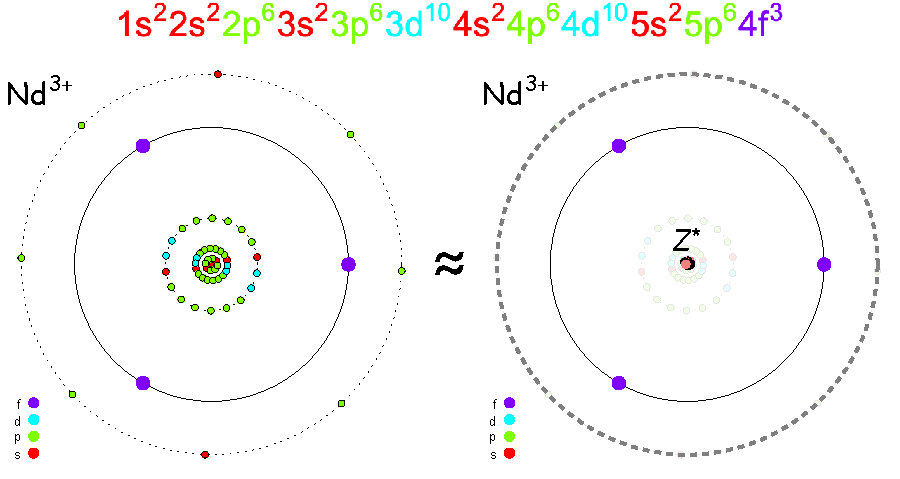
\includegraphics[width=0.85\textwidth]{./figures/nd-3-sketch.pdf}	
\caption{The trivalent neodymium ion shielded by $5s^2$ and $5p^6$ closed shells.}
\label{fig:trivalent-nd-sketch}
\end{figure}


To describe the effect of the charges in the lattice surrounding the ion, the crystal field is introduced. In the simplest of embodiments, the crystal field is simply seen as the electrostatic field due to surrounding charges. This model is of limited applicability if taken too literally; however, if only symmetry considerations are assumed, the model is seen to have greater validity but a somewhat less clear physical origin.

The Hilbert space of a multi-electron ion is a vast stage. In principle, a basis for it should have a countable infinity of bound states and an uncountable infinity of unbound states. This is clearly too much to handle, but thankfully, this large stage can be put in some order thanks to the exclusion principle. The exclusion principle (together with that graceful tendency of things to drift downwards the energetic wells) provides the shell structure. This shell structure, in turn, makes it possible that an atom with many electrons, can be described effectively as an aggregate of an inert core, and a fewer active valence electrons.  

Take for instance a triply ionized (or trivalent) neodymium atom, as depicted in \figuref{fig:trivalent-nd-sketch}. In principle, this gives us the daunting task of dealing with the enormous Hilbert space of 57 electrons. However, 54 of them arrange themselves in a xenon core, so that we are only left to deal with only three. Three are still a challenging task, but much less so than  57. Furthermore, the exclusion principle also guides us in what type of orbital we could possibly place these three electrons, in the case of the lanthanide ions, this being the 4f orbitals. But not really, there are many more unoccupied orbitals outside of the xenon core, two of these electrons, if they are willing to pay the energetic price, they could find themselves in a 5d or a 6s orbital.  

%\begin{table}
%\centering
%    \begin{tabular}{|c|c|}
%        \hline
%        Lanthanide ion & Ground config. \\
%        \hline
%        $\trion{Ce}$ & $\forb^1$ \\ \hline
%        $\trion{Pr}$ & $\forb^2$ \\ \hline
%        $\trion{Nd}$ & $\forb^3$ \\ \hline
%        $\trion{Pm}$ & $\forb^4$ \\ \hline
%        $\trion{Sm}$ & $\forb^5$ \\ \hline  
%        $\trion{Eu}$ & $\forb^6$ \\ \hline
%        $\trion{Gd}$ & $\forb^7$ \\ \hline
%        $\trion{Tb}$ & $\forb^8$ \\ \hline
%        $\trion{Dy}$ & $\forb^9$ \\ \hline
%        $\trion{Ho}$ & $\forb^{10}$ \\ \hline
%        $\trion{Er}$ & $\forb^{11}$ \\ \hline
%        $\trion{Tm}$ & $\forb^{12}$ \\ \hline
%        $\trion{Yb}$ & $\forb^{13}$ \\ \hline
%    \end{tabular}
%    \caption{Ground configuration of trivalent lanthanide ions.}
%    
%\end{table}

\begin{figure}
\centering
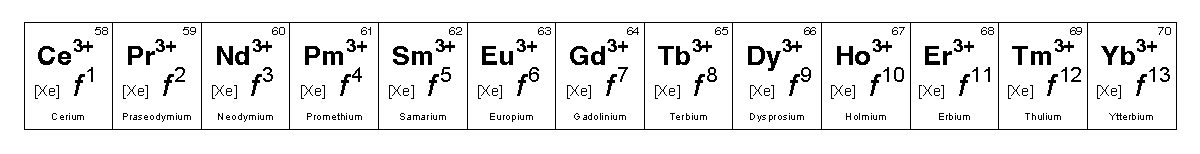
\includegraphics[width=1.\textwidth]{./figures/theLanthanideRow.pdf}
\caption{The trivalent lanthanide row and their ground configurations.}
	\label{figure:tri-lanthanides-row}
\end{figure}


Here we shall assume a single-configuration description. Meaning that all the valence electrons in the ions that we study will all be considered to be located in f-orbitals, or what is the same, that they are described by \fn wavefunctions. \tableref{figure:tri-lanthanides-row} shows the (ground) configuration for the trivalent lanthanide ions. This is, however, a harsh approximation, but thankfully one can make some corrections to it. The effects that arise in the single configuration description because of omitting all the other possible orbitals where the electrons might find themselves, this is what is called \confint.  \index{configuration interaction}

These effects can be brought within the simplified description through perturbation theory. The task not the usual one of correcting for the energies/eigenvectors given an added perturbation, but rather to consider the effects of using a truncated Hilbert space due to a known interaction. For a detailed analysis of this, see Rudzikas' book \cite{rudzikas_theoretical_2007} on theoretical atomic spectroscopy or this article \cite{lindgren_rayleigh-schrodinger_1974} by Lindgren. What results from this analysis are operators that now act solely within the single configuration but with a coefficient that depends on overlap integrals between different configurations. It is from \confint that the parameters $\casimirAlpha, \casimirBeta, \casimirGamma, \Pk{k}, \Tk{k}$ enter into the description.

\begin{mdframed}
\begin{align} 
	& \!\!\!\!\!\!\!\!\!\!\!\! \ham = \underbracket{\hamKineticSymbol}_{\text{kinetic}}
		 + \underbracket{\hamNuclearCoulombSymbol}_{\text{e:shielded nuc}}
		 + \overbrace{\underbracket{\hamSpinOrbitSymbol}_{\text{spin-orbit}}
		 + \underbracket{\hamSpinSpinSymbol}_{
		 			\substack{
		 				\text{spin:spin} \\ 
		 				\text{and spin:other-orbit}
		 				}
		 			} 
         + \underbracket{\hamSOOplusECSOSymbol}_{
            \substack{
                \text{spin:other-orbit} \\ 
                \text{ec-correlated-spin:orbit}
                }
         }
         + \underbracket{\hamZeemanSymbol}_{\text{Zeeman}}}^{\text{magnetic interactions}}  \nonumber \\
         & \!\! \!\! \!\! \!\! \!\!+ \overbrace{\underbracket{\hamCoulombEESymbol}_{\text{e:e}} 
         + \underbracket{\hamTreesSymbol}_\text{Trees effective op} 
		 + \underbracket{\hamGTwoSymbol}_\text{G${}_2$ effective op} 
		 + \underbracket{\hamSOSevenSymbol}_\text{$\SO{7}$ effective op} 
		 + \underbracket{\ham_{\trispoke}}_{\substack{
            \text{effective} \\
            \text{three-body}}}
         + \underbracket{\hamCrystalFieldSymbol}_{\text{crystal field}}}^{\text{electric interactions}} \label{eqn:hamiltonian} \\
	\hamKineticSymbol &= -\frac{\hbar^2}{2m_e}\sum_{i=1}^\numE \nabla_i^2 \text{ (kinetic energy of $\numE$ valence electrons)}\\
	\hamNuclearCoulombSymbol &= \hamNuclearCoulomb \text{ (valence-electrons interaction with shielded nuc. charge)} \\
	\hamSpinOrbitSymbol &= \begin{cases} 
			\hamSpinOrbit \text{ with } \xi{(r_i)} = \frac{\hbar^2}{2 m^2 c^2 r_i} \frac{\diff{V_\text{sn}(r_i)}}{\diff{r_i}} \\
			\sum_{i=1}^\numE \spinZeta \paren{\op{\sspin}_i \cdot \op{\lorb}_i} {{\substack{
						\text{ with $\spinZeta$ the radial average of $\xi(r_i)$} \\ 
						\text{ or used as phenomenological parameter}  
						}
					}}    
			\end{cases} \\    
	\hamSpinSpinSymbol &= \hamSpinSpin \\  
	& \hamSOOplusECSOSymbol = \hamSOOplusECSO \\
    \hamZeemanSymbol &= -\vec{B} \cdot \op{\mu} = \hamZeeman \text{(interaction with a magnetic field)} \\
	\ham_\text{e:e} &= \hamCoulombEE \text{ (repulsion between valence electrons)} \\  
	\nonumber & \text{Let } \casimir{\anyGroup} \DEF \text{The Casimir operator of group $\anyGroup$.}\\ 
	\hamTreesSymbol &= \casimirAlpha\casimir{\SO{3}} = \casimirAlpha \op{L}^2 \text{ (Trees effective operator)} \\
	\hamGTwoSymbol      &= \casimirBeta\casimir{\Gtwo} \\
	\hamSOSevenSymbol   &= \casimirGamma\casimir{\SO{7}} \\
	\ham_{\trispoke} &= {\paramcolor{T'^{(2)}}} \tk{2}' + {\paramcolor{T'^{(11)}}} \tk{11}' + \hamEffectiveThreeBody \text{ (effective 3-body int.)} \\
	\hamCrystalFieldSymbol &= \hamCrystalField \,\,\, {   
		\substack{
			\text{ (crystal field interaction} \\
			\text{with surroundings)}
			} 
			}
\end{align}  
\end{mdframed}

One could try to evaluate the coefficients that result in the Hamiltonian. However, within the \index{semi-empirical approach} \textbf{semi-empirical} approach, these parameters are left to be fitted against experimental data, or at times approximated through Hartree-Fock analysis. This approach is only \textit{semi} empirical in the sense that the model parameters are fitted from experimental data, but the \hamilton that is fitted is based on a clear physical picture inherited from atomic physics.

Putting all of this together leads to the following effective Hamiltonian as show in \eqnref{eqn:hamiltonian}, where ``v-electrons'' is shorthand for valence electrons. It is important to note that the eigenstates that we'll end up with have shoved under the rug all the radial dependence of the wavefunctions. This dependence having been integrated in the parameters of the effective Hamiltonian. The resulting wavefunctions being solely concerned with the angular dependence of the wavefunctions, but modulated by the effects of the radial dependence.



Once all the parameters in this \hamilton have been fitted to experimental data what results is a Hamiltonian such as the one for $\trion{Pr}$ in \LaFthree shown in \figuref{fig:Pr_in_LaF3}. Before we go on to explain in some detail each of the terms included in this Hamiltonian, let us continue to explain the basis used in calculations.

\begin{figure}[h!]
	\begin{center}
		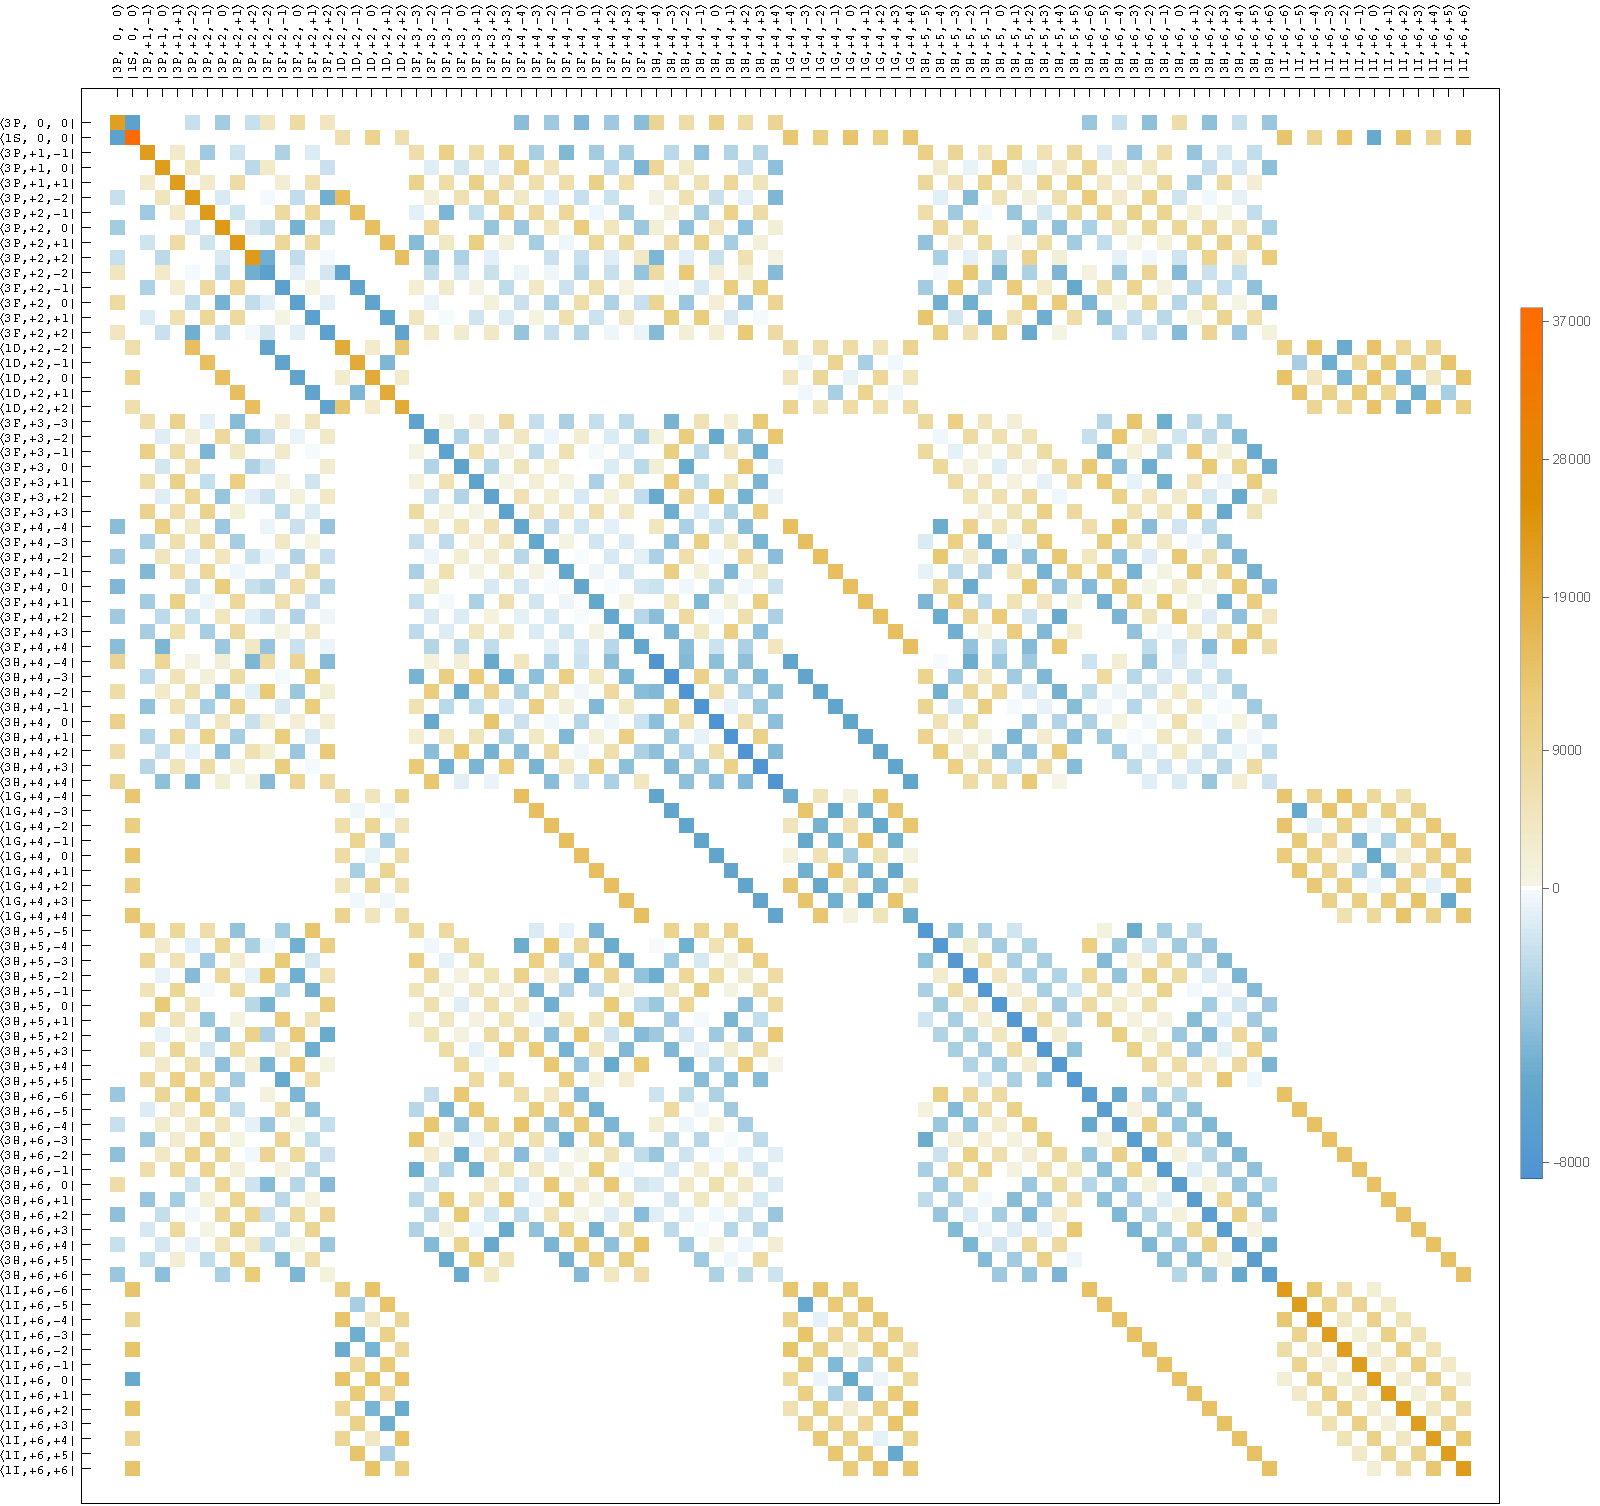
\includegraphics[width=0.95\textwidth]{./figures/Prplot.pdf}
	\end{center}
	\caption{The matrix representation of $\ham$ for $\text{Pr}^{3+}$ in \LaFthree in the $\LSJMbasis$ basis.}
	\label{fig:Pr_in_LaF3} 
\end{figure}

\section{LS coupling basis}\label{section:ls-basis}

In choosing a coupling scheme (or equivalently, choosing a basis in which to represent the Hamiltonian), there are a myriad options; all of them  legitimate in their own right. The art of choosing a useful coupling scheme is that of proposing a basis for the angular part of the wavefunctions that will be close to the actual eigenstates of the system. It being necessary to calculate the matrix elements of the relevant operators, choosing a coupling scheme may also be justified by the easy by which these can be calculated.

\qlanth uses $LS$ coupling for its calculations. In $LS$ coupling all the orbital angular momenta are added to form the total orbital angular momentum $L$, all the spin angular momenta are added to form the total spin angular momentum $S$, and finally these two angular momenta are then added together to form the total angular momentum $J$. The exclusion principle is taken into account in limiting the possible $LS$ terms, and demands no further restrictions. Finally this total angular momentum $J$ is complemented with the quantum number\footnote{A \textit{good} quantum number is any eigenvalue of an operator that commutes with the Hamiltonian; in other words, they are conserved quantities.} $\Msub{J}$ describing the projection of $J$ along the z-axis.

It is worthwhile remembering here the spectroscopic hierarchy of descriptive elements: 
\index{term}\textbf{terms} correspond to $\LSbasis$ (also noted as $\LSterm{2S+1}{L}$), 
\index{level} \textbf{levels} correspond to $\LSJbasis$ (also noted as $\LSJterm{2S+1}{L}{J}$), 
\index{state} and \textbf{states} correspond to $\LSJMbasis$ (also noted as $\LSJMstate{2S+1}{L}{J}{\Msub{J}}$). \figuref{fig: terms-level-states} shows an example of the relationship between a term and its associated levels and states.

In principle the  $\LSJMbasis$ description is the primordial one, the $\LSJbasis$ resulting from neglecting all parts of the Hamiltonian that have no spherical symmetry, and the $\LSbasis$ resulting from further neglecting all terms that couple the spin and orbital angular momenta. Note that a \textit{state} is not an \textit{eigen}-state; all of these are assumed to be basis vectors in the type of description attached to them.

\begin{wrapfigure}{r}{0.4\textwidth}
	\centering
	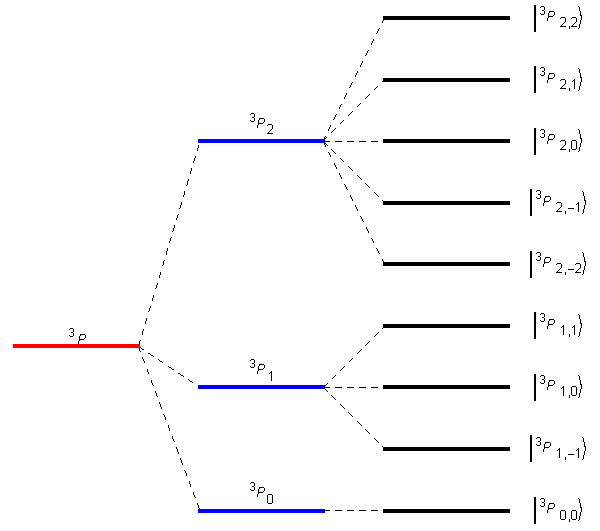
\includegraphics[width=0.4\textwidth]{./figures/term-level-state.pdf}
	\caption{Levels and states associated with the ${}^3\!P$ term in $\underbar{\text{f}}^2$.}
	\label{fig: terms-level-states} 
\end{wrapfigure}

Whereas all four quantum numbers $\LSJMbasis$ are required to specify a state, one may, however, use two simpler descriptions as the situation merits. When all the parts of the Hamiltonian without spherical symmetry are excluded, then a description in terms of $\LSJbasis$ levels is sufficient, the $\Msub{J}$ quantum numbers being redundant and with $J$ being a good quantum number. In a second scenario, when in addition to neglecting all parts without spherical symmetry, one also neglects all parts of the Hamiltonian that couple the spin and orbital degrees of freedom, then the $\LSbasis$ terms constitute the most parsimonious description, with $L$ and $S$ being separately conserved quantities.

When a certain level of description has been adopted one can then assume (at one's own peril) that single states, levels, or terms are actual \textit{eigen}-states/levels/terms of the system at hand. This assumption results in simple transition rules between states/levels/terms. One may, however, within each level of description, take an alternate route, the \textit{intermediate coupling} route, of seeing how the different states/levels/terms mix in the eigenstates found by diagonalizing the appropriate Hamiltonian. This results in a more detailed description at the cost of increased complexity.

\subsection{$\LSJMbasis$ states}

The basis vectors of the $\LSJMbasis$ basis are common eigenvectors of the operators $\op{L}^2$, $\op{S}^2$, $\op{J}^2$, and $\op{J}_z$. They are formed starting from the allowed $LS$ terms in a given configuration, and are then completed with attendant $J$ and $\Msub{J}$ quantum numbers. The $LS$ terms allowed in each configuration $\forb^\numE$ are obtained from tables that originate from the original work by Nielson and Koster \cite{nielson_spectroscopic_1963}. In \qlanth these terms are parsed from the file \codetext{B1F\_ALL.TXT} which is part of the doctoral research of Dobromir Velkov (under the advisory of Brian Judd) \cite{velkov_multi-electron_2000} in which he calculated anew the \cfps. 

One of the facts that have to be accounted for in a basis that uses $L$ and $S$ as quantum numbers, is that there might be several linearly independent paths to couple the electron spin and orbital momenta to add up to given total $L$ and total $S$. For this reason additional labels are necessary to distinguish between these different terms. The simplest way of doing this dates back to the tables of Nielson and Koster \cite{nielson_spectroscopic_1963}, and consists in assigning consecutive integers to degenerate $LS$ terms, with no further meaning to these integers, except that of discriminating between degenerate terms. 
 
The following are all the $LS$ terms in the $\forb^{\numE}$ configurations. In the notation used, the superscript index before the letter notes the spin multiplicity $2S+1$, the roman letter indicates the value of $L$ in spectroscopic notation ($S\!\!\rightarrow\!\!1, P\!\!\rightarrow\!\!2, D\!\!\rightarrow\!\!3, F\!\!\rightarrow\!\!4, G\!\!\rightarrow\!\!5, H\!\!\rightarrow\!\!6, I\!\!\rightarrow\!\!7, K\!\!\rightarrow\!\!8, L\!\!\rightarrow\!\!9, M\!\!\rightarrow\!\!10, N\!\!\rightarrow\!\!11, O\!\!\rightarrow\!\!12, Q\!\!\rightarrow\!\!3, R\!\!\rightarrow\!\!14, T\!\!\rightarrow\!\!15, U\!\!\rightarrow\!\!16, V\!\!\rightarrow\!\!17$), and the final integer (if present) is the label that discriminates between several degenerate $LS$ and must not be confused with a value of $J$. This last index we frequently label in the equations contained in this document with the greek letter $\alpha$ (sadly, for historical reasons, we prepend it, rather than append it).


\begin{mdframed}
\begin{center}
$\forb^{0}$

(1 LS term)
\vspace{0.25cm}
\hrule
\vspace{0.25cm}

$\LSterm{1}{S}$
\end{center}
\end{mdframed}

\begin{mdframed}
\begin{center}
$\forb^{1}$

(1 LS term)
\vspace{0.25cm}
\hrule
\vspace{0.25cm}

$\LSterm{2}{F}$
\end{center}
\end{mdframed}

\begin{mdframed}
\begin{center}
$\forb^{2}$

(7 LS terms)
\vspace{0.25cm}
\hrule
\vspace{0.25cm}

$\LSterm{3}{P}$, $\LSterm{3}{F}$, $\LSterm{3}{H}$, $\LSterm{1}{S}$, $\LSterm{1}{D}$, $\LSterm{1}{G}$, $\LSterm{1}{I}$
\end{center}
\end{mdframed}

\begin{mdframed}
\begin{center}
$\forb^{3}$

(17 LS terms)
\vspace{0.25cm}
\hrule
\vspace{0.25cm}

$\LSterm{4}{S}$, $\LSterm{4}{D}$, $\LSterm{4}{F}$, $\LSterm{4}{G}$, $\LSterm{4}{I}$, $\LSterm{2}{P}$, $\LSterm{2}{D1}$, $\LSterm{2}{D2}$, $\LSterm{2}{F1}$, $\LSterm{2}{F2}$, $\LSterm{2}{G1}$, $\LSterm{2}{G2}$, $\LSterm{2}{H1}$, $\LSterm{2}{H2}$, $\LSterm{2}{I}$, $\LSterm{2}{K}$, $\LSterm{2}{L}$
\end{center}
\end{mdframed}

\begin{mdframed}
\begin{center}
$\forb^{4}$

(47 LS terms)
\vspace{0.25cm}
\hrule
\vspace{0.25cm}

$\LSterm{5}{S}$, $\LSterm{5}{D}$, $\LSterm{5}{F}$, $\LSterm{5}{G}$, $\LSterm{5}{I}$, $\LSterm{3}{P1}$, $\LSterm{3}{P2}$, $\LSterm{3}{P3}$, $\LSterm{3}{D1}$, $\LSterm{3}{D2}$, $\LSterm{3}{F1}$, $\LSterm{3}{F2}$, $\LSterm{3}{F3}$, $\LSterm{3}{F4}$, $\LSterm{3}{G1}$, $\LSterm{3}{G2}$, $\LSterm{3}{G3}$, $\LSterm{3}{H1}$, $\LSterm{3}{H2}$, $\LSterm{3}{H3}$, $\LSterm{3}{H4}$, $\LSterm{3}{I1}$, $\LSterm{3}{I2}$, $\LSterm{3}{K1}$, $\LSterm{3}{K2}$, $\LSterm{3}{L}$, $\LSterm{3}{M}$, $\LSterm{1}{S1}$, $\LSterm{1}{S2}$, $\LSterm{1}{D1}$, $\LSterm{1}{D2}$, $\LSterm{1}{D3}$, $\LSterm{1}{D4}$, $\LSterm{1}{F}$, $\LSterm{1}{G1}$, $\LSterm{1}{G2}$, $\LSterm{1}{G3}$, $\LSterm{1}{G4}$, $\LSterm{1}{H1}$, $\LSterm{1}{H2}$, $\LSterm{1}{I1}$, $\LSterm{1}{I2}$, $\LSterm{1}{I3}$, $\LSterm{1}{K}$, $\LSterm{1}{L1}$, $\LSterm{1}{L2}$, $\LSterm{1}{N}$
\end{center}
\end{mdframed}

\begin{mdframed}
\begin{center}
$\forb^{5}$

(73 LS terms)
\vspace{0.25cm}
\hrule
\vspace{0.25cm}

$\LSterm{6}{P}$, $\LSterm{6}{F}$, $\LSterm{6}{H}$, $\LSterm{4}{S}$, $\LSterm{4}{P1}$, $\LSterm{4}{P2}$, $\LSterm{4}{D1}$, $\LSterm{4}{D2}$, $\LSterm{4}{D3}$, $\LSterm{4}{F1}$, $\LSterm{4}{F2}$, $\LSterm{4}{F3}$, $\LSterm{4}{F4}$, $\LSterm{4}{G1}$, $\LSterm{4}{G2}$, $\LSterm{4}{G3}$, $\LSterm{4}{G4}$, $\LSterm{4}{H1}$, $\LSterm{4}{H2}$, $\LSterm{4}{H3}$, $\LSterm{4}{I1}$, $\LSterm{4}{I2}$, $\LSterm{4}{I3}$, $\LSterm{4}{K1}$, $\LSterm{4}{K2}$, $\LSterm{4}{L}$, $\LSterm{4}{M}$, $\LSterm{2}{P1}$, $\LSterm{2}{P2}$, $\LSterm{2}{P3}$, $\LSterm{2}{P4}$, $\LSterm{2}{D1}$, $\LSterm{2}{D2}$, $\LSterm{2}{D3}$, $\LSterm{2}{D4}$, $\LSterm{2}{D5}$, $\LSterm{2}{F1}$, $\LSterm{2}{F2}$, $\LSterm{2}{F3}$, $\LSterm{2}{F4}$, $\LSterm{2}{F5}$, $\LSterm{2}{F6}$, $\LSterm{2}{F7}$, $\LSterm{2}{G1}$, $\LSterm{2}{G2}$, $\LSterm{2}{G3}$, $\LSterm{2}{G4}$, $\LSterm{2}{G5}$, $\LSterm{2}{G6}$, $\LSterm{2}{H1}$, $\LSterm{2}{H2}$, $\LSterm{2}{H3}$, $\LSterm{2}{H4}$, $\LSterm{2}{H5}$, $\LSterm{2}{H6}$, $\LSterm{2}{H7}$, $\LSterm{2}{I1}$, $\LSterm{2}{I2}$, $\LSterm{2}{I3}$, $\LSterm{2}{I4}$, $\LSterm{2}{I5}$, $\LSterm{2}{K1}$, $\LSterm{2}{K2}$, $\LSterm{2}{K3}$, $\LSterm{2}{K4}$, $\LSterm{2}{K5}$, $\LSterm{2}{L1}$, $\LSterm{2}{L2}$, $\LSterm{2}{L3}$, $\LSterm{2}{M1}$, $\LSterm{2}{M2}$, $\LSterm{2}{N}$, $\LSterm{2}{O}$
\end{center}
\end{mdframed}

\begin{mdframed}
\begin{center}
$\forb^{6}$

(119 LS terms)
\vspace{0.25cm}
\hrule
\vspace{0.25cm}

$\LSterm{7}{F}$, $\LSterm{5}{S}$, $\LSterm{5}{P}$, $\LSterm{5}{D1}$, $\LSterm{5}{D2}$, $\LSterm{5}{D3}$, $\LSterm{5}{F1}$, $\LSterm{5}{F2}$, $\LSterm{5}{G1}$, $\LSterm{5}{G2}$, $\LSterm{5}{G3}$, $\LSterm{5}{H1}$, $\LSterm{5}{H2}$, $\LSterm{5}{I1}$, $\LSterm{5}{I2}$, $\LSterm{5}{K}$, $\LSterm{5}{L}$, $\LSterm{3}{P1}$, $\LSterm{3}{P2}$, $\LSterm{3}{P3}$, $\LSterm{3}{P4}$, $\LSterm{3}{P5}$, $\LSterm{3}{P6}$, $\LSterm{3}{D1}$, $\LSterm{3}{D2}$, $\LSterm{3}{D3}$, $\LSterm{3}{D4}$, $\LSterm{3}{D5}$, $\LSterm{3}{F1}$, $\LSterm{3}{F2}$, $\LSterm{3}{F3}$, $\LSterm{3}{F4}$, $\LSterm{3}{F5}$, $\LSterm{3}{F6}$, $\LSterm{3}{F7}$, $\LSterm{3}{F8}$, $\LSterm{3}{F9}$, $\LSterm{3}{G1}$, $\LSterm{3}{G2}$, $\LSterm{3}{G3}$, $\LSterm{3}{G4}$, $\LSterm{3}{G5}$, $\LSterm{3}{G6}$, $\LSterm{3}{G7}$, $\LSterm{3}{H1}$, $\LSterm{3}{H2}$, $\LSterm{3}{H3}$, $\LSterm{3}{H4}$, $\LSterm{3}{H5}$, $\LSterm{3}{H6}$, $\LSterm{3}{H7}$, $\LSterm{3}{H8}$, $\LSterm{3}{H9}$, $\LSterm{3}{I1}$, $\LSterm{3}{I2}$, $\LSterm{3}{I3}$, $\LSterm{3}{I4}$, $\LSterm{3}{I5}$, $\LSterm{3}{I6}$, $\LSterm{3}{K1}$, $\LSterm{3}{K2}$, $\LSterm{3}{K3}$, $\LSterm{3}{K4}$, $\LSterm{3}{K5}$, $\LSterm{3}{K6}$, $\LSterm{3}{L1}$, $\LSterm{3}{L2}$, $\LSterm{3}{L3}$, $\LSterm{3}{M1}$, $\LSterm{3}{M2}$, $\LSterm{3}{M3}$, $\LSterm{3}{N}$, $\LSterm{3}{O}$, $\LSterm{1}{S1}$, $\LSterm{1}{S2}$, $\LSterm{1}{S3}$, $\LSterm{1}{S4}$, $\LSterm{1}{P}$, $\LSterm{1}{D1}$, $\LSterm{1}{D2}$, $\LSterm{1}{D3}$, $\LSterm{1}{D4}$, $\LSterm{1}{D5}$, $\LSterm{1}{D6}$, $\LSterm{1}{F1}$, $\LSterm{1}{F2}$, $\LSterm{1}{F3}$, $\LSterm{1}{F4}$, $\LSterm{1}{G1}$, $\LSterm{1}{G2}$, $\LSterm{1}{G3}$, $\LSterm{1}{G4}$, $\LSterm{1}{G5}$, $\LSterm{1}{G6}$, $\LSterm{1}{G7}$, $\LSterm{1}{G8}$, $\LSterm{1}{H1}$, $\LSterm{1}{H2}$, $\LSterm{1}{H3}$, $\LSterm{1}{H4}$, $\LSterm{1}{I1}$, $\LSterm{1}{I2}$, $\LSterm{1}{I3}$, $\LSterm{1}{I4}$, $\LSterm{1}{I5}$, $\LSterm{1}{I6}$, $\LSterm{1}{I7}$, $\LSterm{1}{K1}$, $\LSterm{1}{K2}$, $\LSterm{1}{K3}$, $\LSterm{1}{L1}$, $\LSterm{1}{L2}$, $\LSterm{1}{L3}$, $\LSterm{1}{L4}$, $\LSterm{1}{M1}$, $\LSterm{1}{M2}$, $\LSterm{1}{N1}$, $\LSterm{1}{N2}$, $\LSterm{1}{Q}$
\end{center}
\end{mdframed}

\begin{mdframed}
\begin{center}
$\forb^{7}$

(119 LS terms)
\vspace{0.25cm}
\hrule
\vspace{0.25cm}

$\LSterm{8}{S}$, $\LSterm{6}{P}$, $\LSterm{6}{D}$, $\LSterm{6}{F}$, $\LSterm{6}{G}$, $\LSterm{6}{H}$, $\LSterm{6}{I}$, $\LSterm{4}{S1}$, $\LSterm{4}{S2}$, $\LSterm{4}{P1}$, $\LSterm{4}{P2}$, $\LSterm{4}{D1}$, $\LSterm{4}{D2}$, $\LSterm{4}{D3}$, $\LSterm{4}{D4}$, $\LSterm{4}{D5}$, $\LSterm{4}{D6}$, $\LSterm{4}{F1}$, $\LSterm{4}{F2}$, $\LSterm{4}{F3}$, $\LSterm{4}{F4}$, $\LSterm{4}{F5}$, $\LSterm{4}{G1}$, $\LSterm{4}{G2}$, $\LSterm{4}{G3}$, $\LSterm{4}{G4}$, $\LSterm{4}{G5}$, $\LSterm{4}{G6}$, $\LSterm{4}{G7}$, $\LSterm{4}{H1}$, $\LSterm{4}{H2}$, $\LSterm{4}{H3}$, $\LSterm{4}{H4}$, $\LSterm{4}{H5}$, $\LSterm{4}{I1}$, $\LSterm{4}{I2}$, $\LSterm{4}{I3}$, $\LSterm{4}{I4}$, $\LSterm{4}{I5}$, $\LSterm{4}{K1}$, $\LSterm{4}{K2}$, $\LSterm{4}{K3}$, $\LSterm{4}{L1}$, $\LSterm{4}{L2}$, $\LSterm{4}{L3}$, $\LSterm{4}{M}$, $\LSterm{4}{N}$, $\LSterm{2}{S1}$, $\LSterm{2}{S2}$, $\LSterm{2}{P1}$, $\LSterm{2}{P2}$, $\LSterm{2}{P3}$, $\LSterm{2}{P4}$, $\LSterm{2}{P5}$, $\LSterm{2}{D1}$, $\LSterm{2}{D2}$, $\LSterm{2}{D3}$, $\LSterm{2}{D4}$, $\LSterm{2}{D5}$, $\LSterm{2}{D6}$, $\LSterm{2}{D7}$, $\LSterm{2}{F1}$, $\LSterm{2}{F2}$, $\LSterm{2}{F3}$, $\LSterm{2}{F4}$, $\LSterm{2}{F5}$, $\LSterm{2}{F6}$, $\LSterm{2}{F7}$, $\LSterm{2}{F8}$, $\LSterm{2}{F9}$, $\LSterm{2}{F10}$, $\LSterm{2}{G1}$, $\LSterm{2}{G2}$, $\LSterm{2}{G3}$, $\LSterm{2}{G4}$, $\LSterm{2}{G5}$, $\LSterm{2}{G6}$, $\LSterm{2}{G7}$, $\LSterm{2}{G8}$, $\LSterm{2}{G9}$, $\LSterm{2}{G10}$, $\LSterm{2}{H1}$, $\LSterm{2}{H2}$, $\LSterm{2}{H3}$, $\LSterm{2}{H4}$, $\LSterm{2}{H5}$, $\LSterm{2}{H6}$, $\LSterm{2}{H7}$, $\LSterm{2}{H8}$, $\LSterm{2}{H9}$, $\LSterm{2}{I1}$, $\LSterm{2}{I2}$, $\LSterm{2}{I3}$, $\LSterm{2}{I4}$, $\LSterm{2}{I5}$, $\LSterm{2}{I6}$, $\LSterm{2}{I7}$, $\LSterm{2}{I8}$, $\LSterm{2}{I9}$, $\LSterm{2}{K1}$, $\LSterm{2}{K2}$, $\LSterm{2}{K3}$, $\LSterm{2}{K4}$, $\LSterm{2}{K5}$, $\LSterm{2}{K6}$, $\LSterm{2}{K7}$, $\LSterm{2}{L1}$, $\LSterm{2}{L2}$, $\LSterm{2}{L3}$, $\LSterm{2}{L4}$, $\LSterm{2}{L5}$, $\LSterm{2}{M1}$, $\LSterm{2}{M2}$, $\LSterm{2}{M3}$, $\LSterm{2}{M4}$, $\LSterm{2}{N1}$, $\LSterm{2}{N2}$, $\LSterm{2}{O}$, $\LSterm{2}{Q}$
\end{center}
\end{mdframed}

\begin{mdframed}
\begin{center}
$\forb^{8}$

(119 LS terms)
\vspace{0.25cm}
\hrule
\vspace{0.25cm}

$\LSterm{7}{F}$, $\LSterm{5}{S}$, $\LSterm{5}{P}$, $\LSterm{5}{D1}$, $\LSterm{5}{D2}$, $\LSterm{5}{D3}$, $\LSterm{5}{F1}$, $\LSterm{5}{F2}$, $\LSterm{5}{G1}$, $\LSterm{5}{G2}$, $\LSterm{5}{G3}$, $\LSterm{5}{H1}$, $\LSterm{5}{H2}$, $\LSterm{5}{I1}$, $\LSterm{5}{I2}$, $\LSterm{5}{K}$, $\LSterm{5}{L}$, $\LSterm{3}{P1}$, $\LSterm{3}{P2}$, $\LSterm{3}{P3}$, $\LSterm{3}{P4}$, $\LSterm{3}{P5}$, $\LSterm{3}{P6}$, $\LSterm{3}{D1}$, $\LSterm{3}{D2}$, $\LSterm{3}{D3}$, $\LSterm{3}{D4}$, $\LSterm{3}{D5}$, $\LSterm{3}{F1}$, $\LSterm{3}{F2}$, $\LSterm{3}{F3}$, $\LSterm{3}{F4}$, $\LSterm{3}{F5}$, $\LSterm{3}{F6}$, $\LSterm{3}{F7}$, $\LSterm{3}{F8}$, $\LSterm{3}{F9}$, $\LSterm{3}{G1}$, $\LSterm{3}{G2}$, $\LSterm{3}{G3}$, $\LSterm{3}{G4}$, $\LSterm{3}{G5}$, $\LSterm{3}{G6}$, $\LSterm{3}{G7}$, $\LSterm{3}{H1}$, $\LSterm{3}{H2}$, $\LSterm{3}{H3}$, $\LSterm{3}{H4}$, $\LSterm{3}{H5}$, $\LSterm{3}{H6}$, $\LSterm{3}{H7}$, $\LSterm{3}{H8}$, $\LSterm{3}{H9}$, $\LSterm{3}{I1}$, $\LSterm{3}{I2}$, $\LSterm{3}{I3}$, $\LSterm{3}{I4}$, $\LSterm{3}{I5}$, $\LSterm{3}{I6}$, $\LSterm{3}{K1}$, $\LSterm{3}{K2}$, $\LSterm{3}{K3}$, $\LSterm{3}{K4}$, $\LSterm{3}{K5}$, $\LSterm{3}{K6}$, $\LSterm{3}{L1}$, $\LSterm{3}{L2}$, $\LSterm{3}{L3}$, $\LSterm{3}{M1}$, $\LSterm{3}{M2}$, $\LSterm{3}{M3}$, $\LSterm{3}{N}$, $\LSterm{3}{O}$, $\LSterm{1}{S1}$, $\LSterm{1}{S2}$, $\LSterm{1}{S3}$, $\LSterm{1}{S4}$, $\LSterm{1}{P}$, $\LSterm{1}{D1}$, $\LSterm{1}{D2}$, $\LSterm{1}{D3}$, $\LSterm{1}{D4}$, $\LSterm{1}{D5}$, $\LSterm{1}{D6}$, $\LSterm{1}{F1}$, $\LSterm{1}{F2}$, $\LSterm{1}{F3}$, $\LSterm{1}{F4}$, $\LSterm{1}{G1}$, $\LSterm{1}{G2}$, $\LSterm{1}{G3}$, $\LSterm{1}{G4}$, $\LSterm{1}{G5}$, $\LSterm{1}{G6}$, $\LSterm{1}{G7}$, $\LSterm{1}{G8}$, $\LSterm{1}{H1}$, $\LSterm{1}{H2}$, $\LSterm{1}{H3}$, $\LSterm{1}{H4}$, $\LSterm{1}{I1}$, $\LSterm{1}{I2}$, $\LSterm{1}{I3}$, $\LSterm{1}{I4}$, $\LSterm{1}{I5}$, $\LSterm{1}{I6}$, $\LSterm{1}{I7}$, $\LSterm{1}{K1}$, $\LSterm{1}{K2}$, $\LSterm{1}{K3}$, $\LSterm{1}{L1}$, $\LSterm{1}{L2}$, $\LSterm{1}{L3}$, $\LSterm{1}{L4}$, $\LSterm{1}{M1}$, $\LSterm{1}{M2}$, $\LSterm{1}{N1}$, $\LSterm{1}{N2}$, $\LSterm{1}{Q}$
\end{center}
\end{mdframed}

\begin{mdframed}
\begin{center}
$\forb^{9}$

(73 LS terms)
\vspace{0.25cm}
\hrule
\vspace{0.25cm}

$\LSterm{6}{P}$, $\LSterm{6}{F}$, $\LSterm{6}{H}$, $\LSterm{4}{S}$, $\LSterm{4}{P1}$, $\LSterm{4}{P2}$, $\LSterm{4}{D1}$, $\LSterm{4}{D2}$, $\LSterm{4}{D3}$, $\LSterm{4}{F1}$, $\LSterm{4}{F2}$, $\LSterm{4}{F3}$, $\LSterm{4}{F4}$, $\LSterm{4}{G1}$, $\LSterm{4}{G2}$, $\LSterm{4}{G3}$, $\LSterm{4}{G4}$, $\LSterm{4}{H1}$, $\LSterm{4}{H2}$, $\LSterm{4}{H3}$, $\LSterm{4}{I1}$, $\LSterm{4}{I2}$, $\LSterm{4}{I3}$, $\LSterm{4}{K1}$, $\LSterm{4}{K2}$, $\LSterm{4}{L}$, $\LSterm{4}{M}$, $\LSterm{2}{P1}$, $\LSterm{2}{P2}$, $\LSterm{2}{P3}$, $\LSterm{2}{P4}$, $\LSterm{2}{D1}$, $\LSterm{2}{D2}$, $\LSterm{2}{D3}$, $\LSterm{2}{D4}$, $\LSterm{2}{D5}$, $\LSterm{2}{F1}$, $\LSterm{2}{F2}$, $\LSterm{2}{F3}$, $\LSterm{2}{F4}$, $\LSterm{2}{F5}$, $\LSterm{2}{F6}$, $\LSterm{2}{F7}$, $\LSterm{2}{G1}$, $\LSterm{2}{G2}$, $\LSterm{2}{G3}$, $\LSterm{2}{G4}$, $\LSterm{2}{G5}$, $\LSterm{2}{G6}$, $\LSterm{2}{H1}$, $\LSterm{2}{H2}$, $\LSterm{2}{H3}$, $\LSterm{2}{H4}$, $\LSterm{2}{H5}$, $\LSterm{2}{H6}$, $\LSterm{2}{H7}$, $\LSterm{2}{I1}$, $\LSterm{2}{I2}$, $\LSterm{2}{I3}$, $\LSterm{2}{I4}$, $\LSterm{2}{I5}$, $\LSterm{2}{K1}$, $\LSterm{2}{K2}$, $\LSterm{2}{K3}$, $\LSterm{2}{K4}$, $\LSterm{2}{K5}$, $\LSterm{2}{L1}$, $\LSterm{2}{L2}$, $\LSterm{2}{L3}$, $\LSterm{2}{M1}$, $\LSterm{2}{M2}$, $\LSterm{2}{N}$, $\LSterm{2}{O}$
\end{center}
\end{mdframed}

\begin{mdframed}
\begin{center}
$\forb^{10}$

(47 LS terms)
\vspace{0.25cm}
\hrule
\vspace{0.25cm}

$\LSterm{5}{S}$, $\LSterm{5}{D}$, $\LSterm{5}{F}$, $\LSterm{5}{G}$, $\LSterm{5}{I}$, $\LSterm{3}{P1}$, $\LSterm{3}{P2}$, $\LSterm{3}{P3}$, $\LSterm{3}{D1}$, $\LSterm{3}{D2}$, $\LSterm{3}{F1}$, $\LSterm{3}{F2}$, $\LSterm{3}{F3}$, $\LSterm{3}{F4}$, $\LSterm{3}{G1}$, $\LSterm{3}{G2}$, $\LSterm{3}{G3}$, $\LSterm{3}{H1}$, $\LSterm{3}{H2}$, $\LSterm{3}{H3}$, $\LSterm{3}{H4}$, $\LSterm{3}{I1}$, $\LSterm{3}{I2}$, $\LSterm{3}{K1}$, $\LSterm{3}{K2}$, $\LSterm{3}{L}$, $\LSterm{3}{M}$, $\LSterm{1}{S1}$, $\LSterm{1}{S2}$, $\LSterm{1}{D1}$, $\LSterm{1}{D2}$, $\LSterm{1}{D3}$, $\LSterm{1}{D4}$, $\LSterm{1}{F}$, $\LSterm{1}{G1}$, $\LSterm{1}{G2}$, $\LSterm{1}{G3}$, $\LSterm{1}{G4}$, $\LSterm{1}{H1}$, $\LSterm{1}{H2}$, $\LSterm{1}{I1}$, $\LSterm{1}{I2}$, $\LSterm{1}{I3}$, $\LSterm{1}{K}$, $\LSterm{1}{L1}$, $\LSterm{1}{L2}$, $\LSterm{1}{N}$
\end{center}
\end{mdframed}

\begin{mdframed}
\begin{center}
$\forb^{11}$

(17 LS terms)
\vspace{0.25cm}
\hrule
\vspace{0.25cm}

$\LSterm{4}{S}$, $\LSterm{4}{D}$, $\LSterm{4}{F}$, $\LSterm{4}{G}$, $\LSterm{4}{I}$, $\LSterm{2}{P}$, $\LSterm{2}{D1}$, $\LSterm{2}{D2}$, $\LSterm{2}{F1}$, $\LSterm{2}{F2}$, $\LSterm{2}{G1}$, $\LSterm{2}{G2}$, $\LSterm{2}{H1}$, $\LSterm{2}{H2}$, $\LSterm{2}{I}$, $\LSterm{2}{K}$, $\LSterm{2}{L}$
\end{center}
\end{mdframed}

\begin{mdframed}
\begin{center}
$\forb^{12}$

(7 LS terms)
\vspace{0.25cm}
\hrule
\vspace{0.25cm}

$\LSterm{3}{P}$, $\LSterm{3}{F}$, $\LSterm{3}{H}$, $\LSterm{1}{S}$, $\LSterm{1}{D}$, $\LSterm{1}{G}$, $\LSterm{1}{I}$
\end{center}
\end{mdframed}

\begin{mdframed}
\begin{center}
$\forb^{13}$

(1 LS term)
\vspace{0.25cm}
\hrule
\vspace{0.25cm}

$\LSterm{2}{F}$
\end{center}
\end{mdframed}

\begin{mdframed}
\begin{center}
$\forb^{14}$

(1 LS term)
\vspace{0.25cm}
\hrule
\vspace{0.25cm}

$\LSterm{1}{S}$
\end{center}
\end{mdframed}

 
 
 
In \qlanth these terms may be queried through the function \codetext{AllowedNKSLTerms}. 

\foreach \name in {AllowedNKSLTerms}{ 
        \lstinputlisting[language=Mathematica]{./fundefs/\name.tex}
    }

In addition to $LS$, the $\LSJMbasis$ basis states are also specified by the total angular momentum $J$ (which may go from $\abs{L-S}$ to $\abs{L+S}$). Then for each $J$, there are $2J+1$ projections on the z-axis. For example, the ordered $\LSJMbasis$ basis for $\forb^2$ is shown below, where the first element is the $LS$ term given as a string, the second equal to $J$, and the third one equal to $\Msub{J}$:
 

\begin{mdframed}
\begin{center}
$(J=0)$


(2 kets)
\vspace{0.25cm}\hrule\vspace{0.25cm}
$\ket{\LSterm{3}{P},0,0}$, $\ket{\LSterm{1}{S},0,0}$
\end{center}
\end{mdframed}

\begin{mdframed}
\begin{center}
$(J=1)$


(3 kets)
\vspace{0.25cm}\hrule\vspace{0.25cm}
$\ket{\LSterm{3}{P},1,-1}$, $\ket{\LSterm{3}{P},1,0}$, $\ket{\LSterm{3}{P},1,1}$
\end{center}
\end{mdframed}

\begin{mdframed}
\begin{center}
$(J=2)$


(15 kets)
\vspace{0.25cm}\hrule\vspace{0.25cm}
$\ket{\LSterm{3}{P},2,-2}$, $\ket{\LSterm{3}{P},2,-1}$, $\ket{\LSterm{3}{P},2,0}$, $\ket{\LSterm{3}{P},2,1}$, $\ket{\LSterm{3}{P},2,2}$, $\ket{\LSterm{3}{F},2,-2}$, $\ket{\LSterm{3}{F},2,-1}$, $\ket{\LSterm{3}{F},2,0}$, $\ket{\LSterm{3}{F},2,1}$, $\ket{\LSterm{3}{F},2,2}$, $\ket{\LSterm{1}{D},2,-2}$, $\ket{\LSterm{1}{D},2,-1}$, $\ket{\LSterm{1}{D},2,0}$, $\ket{\LSterm{1}{D},2,1}$, $\ket{\LSterm{1}{D},2,2}$
\end{center}
\end{mdframed}

\begin{mdframed}
\begin{center}
$(J=3)$


(7 kets)
\vspace{0.25cm}\hrule\vspace{0.25cm}
$\ket{\LSterm{3}{F},3,-3}$, $\ket{\LSterm{3}{F},3,-2}$, $\ket{\LSterm{3}{F},3,-1}$, $\ket{\LSterm{3}{F},3,0}$, $\ket{\LSterm{3}{F},3,1}$, $\ket{\LSterm{3}{F},3,2}$, $\ket{\LSterm{3}{F},3,3}$
\end{center}
\end{mdframed}

\begin{mdframed}
\begin{center}
$(J=4)$


(27 kets)
\vspace{0.25cm}\hrule\vspace{0.25cm}
$\ket{\LSterm{3}{F},4,-4}$, $\ket{\LSterm{3}{F},4,-3}$, $\ket{\LSterm{3}{F},4,-2}$, $\ket{\LSterm{3}{F},4,-1}$, $\ket{\LSterm{3}{F},4,0}$, $\ket{\LSterm{3}{F},4,1}$, $\ket{\LSterm{3}{F},4,2}$, $\ket{\LSterm{3}{F},4,3}$, $\ket{\LSterm{3}{F},4,4}$, $\ket{\LSterm{3}{H},4,-4}$, $\ket{\LSterm{3}{H},4,-3}$, $\ket{\LSterm{3}{H},4,-2}$, $\ket{\LSterm{3}{H},4,-1}$, $\ket{\LSterm{3}{H},4,0}$, $\ket{\LSterm{3}{H},4,1}$, $\ket{\LSterm{3}{H},4,2}$, $\ket{\LSterm{3}{H},4,3}$, $\ket{\LSterm{3}{H},4,4}$, $\ket{\LSterm{1}{G},4,-4}$, $\ket{\LSterm{1}{G},4,-3}$, $\ket{\LSterm{1}{G},4,-2}$, $\ket{\LSterm{1}{G},4,-1}$, $\ket{\LSterm{1}{G},4,0}$, $\ket{\LSterm{1}{G},4,1}$, $\ket{\LSterm{1}{G},4,2}$, $\ket{\LSterm{1}{G},4,3}$, $\ket{\LSterm{1}{G},4,4}$
\end{center}
\end{mdframed}

\begin{mdframed}
\begin{center}
$(J=5)$


(11 kets)
\vspace{0.25cm}\hrule\vspace{0.25cm}
$\ket{\LSterm{3}{H},5,-5}$, $\ket{\LSterm{3}{H},5,-4}$, $\ket{\LSterm{3}{H},5,-3}$, $\ket{\LSterm{3}{H},5,-2}$, $\ket{\LSterm{3}{H},5,-1}$, $\ket{\LSterm{3}{H},5,0}$, $\ket{\LSterm{3}{H},5,1}$, $\ket{\LSterm{3}{H},5,2}$, $\ket{\LSterm{3}{H},5,3}$, $\ket{\LSterm{3}{H},5,4}$, $\ket{\LSterm{3}{H},5,5}$
\end{center}
\end{mdframed}

\begin{mdframed}
\begin{center}
$(J=6)$


(26 kets)
\vspace{0.25cm}\hrule\vspace{0.25cm}
$\ket{\LSterm{3}{H},6,-6}$, $\ket{\LSterm{3}{H},6,-5}$, $\ket{\LSterm{3}{H},6,-4}$, $\ket{\LSterm{3}{H},6,-3}$, $\ket{\LSterm{3}{H},6,-2}$, $\ket{\LSterm{3}{H},6,-1}$, $\ket{\LSterm{3}{H},6,0}$, $\ket{\LSterm{3}{H},6,1}$, $\ket{\LSterm{3}{H},6,2}$, $\ket{\LSterm{3}{H},6,3}$, $\ket{\LSterm{3}{H},6,4}$, $\ket{\LSterm{3}{H},6,5}$, $\ket{\LSterm{3}{H},6,6}$, $\ket{\LSterm{1}{I},6,-6}$, $\ket{\LSterm{1}{I},6,-5}$, $\ket{\LSterm{1}{I},6,-4}$, $\ket{\LSterm{1}{I},6,-3}$, $\ket{\LSterm{1}{I},6,-2}$, $\ket{\LSterm{1}{I},6,-1}$, $\ket{\LSterm{1}{I},6,0}$, $\ket{\LSterm{1}{I},6,1}$, $\ket{\LSterm{1}{I},6,2}$, $\ket{\LSterm{1}{I},6,3}$, $\ket{\LSterm{1}{I},6,4}$, $\ket{\LSterm{1}{I},6,5}$, $\ket{\LSterm{1}{I},6,6}$
\end{center}
\end{mdframed} 


The order above is an example of the bases ordering used in \qlanth. Notice how the basis vectors are sorted in order of increasing $J$, so that for instance not all of the basis states associated with the $\LSterm{3}{P}$ $LS$ term are contiguous. Within each group for a given $J$ the basis kets are then ordered in decreasing $S$, then ordered in increasing $L$, and then according to $\Msub{J}$.

In \qlanth the ordered basis used for a given $\forb^\numE$ is provided by \codetext{BasisLSJMJ} which provides a list with $\binom{14}{n}$ elements.

\lstinputlisting[language=Mathematica]{./fundefs/BasisLSJMJ.tex}

\subsection{More quantum numbers}

Besides using an integer which solves the problem of discriminating between degenerate $LS$ terms by enumerating them, it is also possible to add more useful labels that reflect additional symmetries that the f-electron basis states have in the groups $\SO{7}$ (the Lie group of rotations in seven dimensions) and $\Gtwo$ (the rank-2 exceptional simple Lie group).

\subsubsection{Seniority $\senior$}

The seniority number connects different $LS$ terms between configurations, so that a term below can be seen as the \textit{senior} of a term above. To determine the seniority of a given term in configuration $\forb^\numE$, one must first find the configuration $\forb^{\tilde{\numE}}$ in which this term appeared. For example, $\forb^{5}$ contains six degenerate ${}^2G$ terms. The first time this term appeared was in $\forb^3$, where it had a degeneracy of 2. The 2 degenerate terms in $\forb^3$ would then both have a seniority of $\senior=3$ since they first appeared in $\forb^3$. In consequence two of the six degenerate terms in $\forb^5$ would have the same degeneracy those two in $\forb^3$, and are therefore linked to those previous two. The four remaining ones, are  considered to be \textit{born} in $\forb^5$, and therefore have a seniority $\senior=5$.

These rules seem to be ad-hoc, but they are useful in dealing with the degeneracies in the $LS$ terms as they arrive going up the configurations. It provides a useful way of tracking what happens to each \textit{branch} of the coupling tree as it grows and withers with increasing number of electrons.

There is, however, a deeper meaning to the seniority number. It can be shown that the seniority number (more exactly a quantity related to it) is a sort of spin, a \textit{quasi}-spin, where the spin projections along the `z-axis' correspond to different number of electrons in $\forb^\numE$ configurations \cite{judd_second_1967}. This is a consequence of the exclusion principle. It is also useful to relate matrix elements of operators in one configuration to those in another, through the use of the Wigner-Eckart theorem. This is an interesting and useful theoretical construct, but the method of fractional parentage (which is what is implemented in $\qlanth$) is equally adequate, albeit being somewhat less parsimonious than what the quasi-spin view that seniority can provide. As such $\qlanth$ does not use the seniority numbers that are associated with each $LS$ term\footnote{Except for calculating the coefficients of fractional parentage beyond $\forb^7$, which are useful, but not essential to the calculations of \qlanth.}. However, in \qlanth the seniority of a given $LS$ term can be obtained using the function \codetext{Seniority}.

\lstinputlisting[language=Mathematica]{./fundefs/Seniority.tex} 

\subsubsection{$\RacahU$ and $\RacahW$}

Much as $L$ tells us how a rotation acts on an $L$ wavefunction by mixing different $\Msub{L}$ components, these other two quantum numbers specify how the wavefunctions transform under the operations of two other two groups. The $\RacahW$ label determines how a wavefunction transforms under a rotation in 7-dimensional space, and $\RacahU$ how they transform under an operator of group $\Gtwo$. Without going into the group theoretical details, the irreducible representations of $\SO{7}$ can be represented by triples of integer numbers, and those of $\Gtwo$ as pairs of two integers.

In \qlanth the $\RacahW$ and $\RacahU$ are used in order to determine the matrix elements of the $\casimir{\SO{7}}$ and $\casimir{\Gtwo}$ Casimir operators. These labels can be retrieved, for a given $LS$ string, using the function \codetext{FindNKLSTerm}.

\lstinputlisting[language=Mathematica]{./fundefs/FindNKLSTerm.tex} 


\subsection{$\LSJbasis$ levels}

When the Hamiltonian only includes spherically symmetric terms (or what is the same, when the crystal field is neglected) then the $\Msub{J}$ quantum numbers in the $\LSJMbasis$ basis states are redundant. This permits a simplified description  in terms of $\LSJbasis$ levels. The following are the different $\LSJterm{2S+1}{L}{J}$ levels that span the eigenvectors that result from diagonalizing the Hamiltonian in the level description, these may also be termed \textit{multiplets}. (In these we have excluded the indices that distinguish between degenerate LS terms)

\begin{mdframed}
\begin{center}
$\forb^{1}$
(2 LSJ levels)
\vspace{0.25cm}
\hrule
\vspace{0.25cm}

$\LSJterm{2}{F}{5/2}$, $\LSJterm{2}{F}{7/2}$
\end{center}
\end{mdframed}


\begin{mdframed}
\begin{center}
$\forb^{2}$
(13 LSJ levels)
\vspace{0.25cm}
\hrule
\vspace{0.25cm}

$\LSJterm{3}{P}{0}$, $\LSJterm{1}{S}{0}$, $\LSJterm{3}{P}{1}$, $\LSJterm{3}{P}{2}$, $\LSJterm{3}{F}{2}$, $\LSJterm{1}{D}{2}$, $\LSJterm{3}{F}{3}$, $\LSJterm{3}{F}{4}$, $\LSJterm{3}{H}{4}$, $\LSJterm{1}{G}{4}$, $\LSJterm{3}{H}{5}$, $\LSJterm{3}{H}{6}$, $\LSJterm{1}{I}{6}$
\end{center}
\end{mdframed}


\begin{mdframed}
\begin{center}
$\forb^{3}$
(41 LSJ levels)
\vspace{0.25cm}
\hrule
\vspace{0.25cm}

$\LSJterm{4}{D}{1/2}$, $\LSJterm{2}{P}{1/2}$, $\LSJterm{4}{S}{3/2}$, $\LSJterm{4}{D}{3/2}$, $\LSJterm{4}{F}{3/2}$, $\LSJterm{2}{P}{3/2}$, $\LSJterm{2}{D}{3/2}$, $\LSJterm{2}{D}{3/2}$, $\LSJterm{4}{D}{5/2}$, $\LSJterm{4}{F}{5/2}$, $\LSJterm{4}{G}{5/2}$, $\LSJterm{2}{D}{5/2}$, $\LSJterm{2}{D}{5/2}$, $\LSJterm{2}{F}{5/2}$, $\LSJterm{2}{F}{5/2}$, $\LSJterm{4}{D}{7/2}$, $\LSJterm{4}{F}{7/2}$, $\LSJterm{4}{G}{7/2}$, $\LSJterm{2}{F}{7/2}$, $\LSJterm{2}{F}{7/2}$, $\LSJterm{2}{G}{7/2}$, $\LSJterm{2}{G}{7/2}$, $\LSJterm{4}{F}{9/2}$, $\LSJterm{4}{G}{9/2}$, $\LSJterm{4}{I}{9/2}$, $\LSJterm{2}{G}{9/2}$, $\LSJterm{2}{G}{9/2}$, $\LSJterm{2}{H}{9/2}$, $\LSJterm{2}{H}{9/2}$, $\LSJterm{4}{G}{11/2}$, $\LSJterm{4}{I}{11/2}$, $\LSJterm{2}{H}{11/2}$, $\LSJterm{2}{H}{11/2}$, $\LSJterm{2}{I}{11/2}$, $\LSJterm{4}{I}{13/2}$, $\LSJterm{2}{I}{13/2}$, $\LSJterm{2}{K}{13/2}$, $\LSJterm{4}{I}{15/2}$, $\LSJterm{2}{K}{15/2}$, $\LSJterm{2}{L}{15/2}$, $\LSJterm{2}{L}{17/2}$
\end{center}
\end{mdframed}


\begin{mdframed}
\begin{center}
$\forb^{4}$
(107 LSJ levels)
\vspace{0.25cm}
\hrule
\vspace{0.25cm}

$\LSJterm{5}{D}{0}$, $\LSJterm{3}{P}{0}$, $\LSJterm{3}{P}{0}$, $\LSJterm{3}{P}{0}$, $\LSJterm{1}{S}{0}$, $\LSJterm{1}{S}{0}$, $\LSJterm{5}{D}{1}$, $\LSJterm{5}{F}{1}$, $\LSJterm{3}{P}{1}$, $\LSJterm{3}{P}{1}$, $\LSJterm{3}{P}{1}$, $\LSJterm{3}{D}{1}$, $\LSJterm{3}{D}{1}$, $\LSJterm{5}{S}{2}$, $\LSJterm{5}{D}{2}$, $\LSJterm{5}{F}{2}$, $\LSJterm{5}{G}{2}$, $\LSJterm{3}{P}{2}$, $\LSJterm{3}{P}{2}$, $\LSJterm{3}{P}{2}$, $\LSJterm{3}{D}{2}$, $\LSJterm{3}{D}{2}$, $\LSJterm{3}{F}{2}$, $\LSJterm{3}{F}{2}$, $\LSJterm{3}{F}{2}$, $\LSJterm{3}{F}{2}$, $\LSJterm{1}{D}{2}$, $\LSJterm{1}{D}{2}$, $\LSJterm{1}{D}{2}$, $\LSJterm{1}{D}{2}$, $\LSJterm{5}{D}{3}$, $\LSJterm{5}{F}{3}$, $\LSJterm{5}{G}{3}$, $\LSJterm{3}{D}{3}$, $\LSJterm{3}{D}{3}$, $\LSJterm{3}{F}{3}$, $\LSJterm{3}{F}{3}$, $\LSJterm{3}{F}{3}$, $\LSJterm{3}{F}{3}$, $\LSJterm{3}{G}{3}$, $\LSJterm{3}{G}{3}$, $\LSJterm{3}{G}{3}$, $\LSJterm{1}{F}{3}$, $\LSJterm{5}{D}{4}$, $\LSJterm{5}{F}{4}$, $\LSJterm{5}{G}{4}$, $\LSJterm{5}{I}{4}$, $\LSJterm{3}{F}{4}$, $\LSJterm{3}{F}{4}$, $\LSJterm{3}{F}{4}$, $\LSJterm{3}{F}{4}$, $\LSJterm{3}{G}{4}$, $\LSJterm{3}{G}{4}$, $\LSJterm{3}{G}{4}$, $\LSJterm{3}{H}{4}$, $\LSJterm{3}{H}{4}$, $\LSJterm{3}{H}{4}$, $\LSJterm{3}{H}{4}$, $\LSJterm{1}{G}{4}$, $\LSJterm{1}{G}{4}$, $\LSJterm{1}{G}{4}$, $\LSJterm{1}{G}{4}$, $\LSJterm{5}{F}{5}$, $\LSJterm{5}{G}{5}$, $\LSJterm{5}{I}{5}$, $\LSJterm{3}{G}{5}$, $\LSJterm{3}{G}{5}$, $\LSJterm{3}{G}{5}$, $\LSJterm{3}{H}{5}$, $\LSJterm{3}{H}{5}$, $\LSJterm{3}{H}{5}$, $\LSJterm{3}{H}{5}$, $\LSJterm{3}{I}{5}$, $\LSJterm{3}{I}{5}$, $\LSJterm{1}{H}{5}$, $\LSJterm{1}{H}{5}$, $\LSJterm{5}{G}{6}$, $\LSJterm{5}{I}{6}$, $\LSJterm{3}{H}{6}$, $\LSJterm{3}{H}{6}$, $\LSJterm{3}{H}{6}$, $\LSJterm{3}{H}{6}$, $\LSJterm{3}{I}{6}$, $\LSJterm{3}{I}{6}$, $\LSJterm{3}{K}{6}$, $\LSJterm{3}{K}{6}$, $\LSJterm{1}{I}{6}$, $\LSJterm{1}{I}{6}$, $\LSJterm{1}{I}{6}$, $\LSJterm{5}{I}{7}$, $\LSJterm{3}{I}{7}$, $\LSJterm{3}{I}{7}$, $\LSJterm{3}{K}{7}$, $\LSJterm{3}{K}{7}$, $\LSJterm{3}{L}{7}$, $\LSJterm{1}{K}{7}$, $\LSJterm{5}{I}{8}$, $\LSJterm{3}{K}{8}$, $\LSJterm{3}{K}{8}$, $\LSJterm{3}{L}{8}$, $\LSJterm{3}{M}{8}$, $\LSJterm{1}{L}{8}$, $\LSJterm{1}{L}{8}$, $\LSJterm{3}{L}{9}$, $\LSJterm{3}{M}{9}$, $\LSJterm{3}{M}{10}$, $\LSJterm{1}{N}{10}$
\end{center}
\end{mdframed}


\begin{mdframed}
\begin{center}
$\forb^{5}$
(198 LSJ levels)
\vspace{0.25cm}
\hrule
\vspace{0.25cm}

$\LSJterm{6}{F}{1/2}$, $\LSJterm{4}{P}{1/2}$, $\LSJterm{4}{P}{1/2}$, $\LSJterm{4}{D}{1/2}$, $\LSJterm{4}{D}{1/2}$, $\LSJterm{4}{D}{1/2}$, $\LSJterm{2}{P}{1/2}$, $\LSJterm{2}{P}{1/2}$, $\LSJterm{2}{P}{1/2}$, $\LSJterm{2}{P}{1/2}$, $\LSJterm{6}{P}{3/2}$, $\LSJterm{6}{F}{3/2}$, $\LSJterm{4}{S}{3/2}$, $\LSJterm{4}{P}{3/2}$, $\LSJterm{4}{P}{3/2}$, $\LSJterm{4}{D}{3/2}$, $\LSJterm{4}{D}{3/2}$, $\LSJterm{4}{D}{3/2}$, $\LSJterm{4}{F}{3/2}$, $\LSJterm{4}{F}{3/2}$, $\LSJterm{4}{F}{3/2}$, $\LSJterm{4}{F}{3/2}$, $\LSJterm{2}{P}{3/2}$, $\LSJterm{2}{P}{3/2}$, $\LSJterm{2}{P}{3/2}$, $\LSJterm{2}{P}{3/2}$, $\LSJterm{2}{D}{3/2}$, $\LSJterm{2}{D}{3/2}$, $\LSJterm{2}{D}{3/2}$, $\LSJterm{2}{D}{3/2}$, $\LSJterm{2}{D}{3/2}$, $\LSJterm{6}{P}{5/2}$, $\LSJterm{6}{F}{5/2}$, $\LSJterm{6}{H}{5/2}$, $\LSJterm{4}{P}{5/2}$, $\LSJterm{4}{P}{5/2}$, $\LSJterm{4}{D}{5/2}$, $\LSJterm{4}{D}{5/2}$, $\LSJterm{4}{D}{5/2}$, $\LSJterm{4}{F}{5/2}$, $\LSJterm{4}{F}{5/2}$, $\LSJterm{4}{F}{5/2}$, $\LSJterm{4}{F}{5/2}$, $\LSJterm{4}{G}{5/2}$, $\LSJterm{4}{G}{5/2}$, $\LSJterm{4}{G}{5/2}$, $\LSJterm{4}{G}{5/2}$, $\LSJterm{2}{D}{5/2}$, $\LSJterm{2}{D}{5/2}$, $\LSJterm{2}{D}{5/2}$, $\LSJterm{2}{D}{5/2}$, $\LSJterm{2}{D}{5/2}$, $\LSJterm{2}{F}{5/2}$, $\LSJterm{2}{F}{5/2}$, $\LSJterm{2}{F}{5/2}$, $\LSJterm{2}{F}{5/2}$, $\LSJterm{2}{F}{5/2}$, $\LSJterm{2}{F}{5/2}$, $\LSJterm{2}{F}{5/2}$, $\LSJterm{6}{P}{7/2}$, $\LSJterm{6}{F}{7/2}$, $\LSJterm{6}{H}{7/2}$, $\LSJterm{4}{D}{7/2}$, $\LSJterm{4}{D}{7/2}$, $\LSJterm{4}{D}{7/2}$, $\LSJterm{4}{F}{7/2}$, $\LSJterm{4}{F}{7/2}$, $\LSJterm{4}{F}{7/2}$, $\LSJterm{4}{F}{7/2}$, $\LSJterm{4}{G}{7/2}$, $\LSJterm{4}{G}{7/2}$, $\LSJterm{4}{G}{7/2}$, $\LSJterm{4}{G}{7/2}$, $\LSJterm{4}{H}{7/2}$, $\LSJterm{4}{H}{7/2}$, $\LSJterm{4}{H}{7/2}$, $\LSJterm{2}{F}{7/2}$, $\LSJterm{2}{F}{7/2}$, $\LSJterm{2}{F}{7/2}$, $\LSJterm{2}{F}{7/2}$, $\LSJterm{2}{F}{7/2}$, $\LSJterm{2}{F}{7/2}$, $\LSJterm{2}{F}{7/2}$, $\LSJterm{2}{G}{7/2}$, $\LSJterm{2}{G}{7/2}$, $\LSJterm{2}{G}{7/2}$, $\LSJterm{2}{G}{7/2}$, $\LSJterm{2}{G}{7/2}$, $\LSJterm{2}{G}{7/2}$, $\LSJterm{6}{F}{9/2}$, $\LSJterm{6}{H}{9/2}$, $\LSJterm{4}{F}{9/2}$, $\LSJterm{4}{F}{9/2}$, $\LSJterm{4}{F}{9/2}$, $\LSJterm{4}{F}{9/2}$, $\LSJterm{4}{G}{9/2}$, $\LSJterm{4}{G}{9/2}$, $\LSJterm{4}{G}{9/2}$, $\LSJterm{4}{G}{9/2}$, $\LSJterm{4}{H}{9/2}$, $\LSJterm{4}{H}{9/2}$, $\LSJterm{4}{H}{9/2}$, $\LSJterm{4}{I}{9/2}$, $\LSJterm{4}{I}{9/2}$, $\LSJterm{4}{I}{9/2}$, $\LSJterm{2}{G}{9/2}$, $\LSJterm{2}{G}{9/2}$, $\LSJterm{2}{G}{9/2}$, $\LSJterm{2}{G}{9/2}$, $\LSJterm{2}{G}{9/2}$, $\LSJterm{2}{G}{9/2}$, $\LSJterm{2}{H}{9/2}$, $\LSJterm{2}{H}{9/2}$, $\LSJterm{2}{H}{9/2}$, $\LSJterm{2}{H}{9/2}$, $\LSJterm{2}{H}{9/2}$, $\LSJterm{2}{H}{9/2}$, $\LSJterm{2}{H}{9/2}$, $\LSJterm{6}{F}{11/2}$, $\LSJterm{6}{H}{11/2}$, $\LSJterm{4}{G}{11/2}$, $\LSJterm{4}{G}{11/2}$, $\LSJterm{4}{G}{11/2}$, $\LSJterm{4}{G}{11/2}$, $\LSJterm{4}{H}{11/2}$, $\LSJterm{4}{H}{11/2}$, $\LSJterm{4}{H}{11/2}$, $\LSJterm{4}{I}{11/2}$, $\LSJterm{4}{I}{11/2}$, $\LSJterm{4}{I}{11/2}$, $\LSJterm{4}{K}{11/2}$, $\LSJterm{4}{K}{11/2}$, $\LSJterm{2}{H}{11/2}$, $\LSJterm{2}{H}{11/2}$, $\LSJterm{2}{H}{11/2}$, $\LSJterm{2}{H}{11/2}$, $\LSJterm{2}{H}{11/2}$, $\LSJterm{2}{H}{11/2}$, $\LSJterm{2}{H}{11/2}$, $\LSJterm{2}{I}{11/2}$, $\LSJterm{2}{I}{11/2}$, $\LSJterm{2}{I}{11/2}$, $\LSJterm{2}{I}{11/2}$, $\LSJterm{2}{I}{11/2}$, $\LSJterm{6}{H}{13/2}$, $\LSJterm{4}{H}{13/2}$, $\LSJterm{4}{H}{13/2}$, $\LSJterm{4}{H}{13/2}$, $\LSJterm{4}{I}{13/2}$, $\LSJterm{4}{I}{13/2}$, $\LSJterm{4}{I}{13/2}$, $\LSJterm{4}{K}{13/2}$, $\LSJterm{4}{K}{13/2}$, $\LSJterm{4}{L}{13/2}$, $\LSJterm{2}{I}{13/2}$, $\LSJterm{2}{I}{13/2}$, $\LSJterm{2}{I}{13/2}$, $\LSJterm{2}{I}{13/2}$, $\LSJterm{2}{I}{13/2}$, $\LSJterm{2}{K}{13/2}$, $\LSJterm{2}{K}{13/2}$, $\LSJterm{2}{K}{13/2}$, $\LSJterm{2}{K}{13/2}$, $\LSJterm{2}{K}{13/2}$, $\LSJterm{6}{H}{15/2}$, $\LSJterm{4}{I}{15/2}$, $\LSJterm{4}{I}{15/2}$, $\LSJterm{4}{I}{15/2}$, $\LSJterm{4}{K}{15/2}$, $\LSJterm{4}{K}{15/2}$, $\LSJterm{4}{L}{15/2}$, $\LSJterm{4}{M}{15/2}$, $\LSJterm{2}{K}{15/2}$, $\LSJterm{2}{K}{15/2}$, $\LSJterm{2}{K}{15/2}$, $\LSJterm{2}{K}{15/2}$, $\LSJterm{2}{K}{15/2}$, $\LSJterm{2}{L}{15/2}$, $\LSJterm{2}{L}{15/2}$, $\LSJterm{2}{L}{15/2}$, $\LSJterm{4}{K}{17/2}$, $\LSJterm{4}{K}{17/2}$, $\LSJterm{4}{L}{17/2}$, $\LSJterm{4}{M}{17/2}$, $\LSJterm{2}{L}{17/2}$, $\LSJterm{2}{L}{17/2}$, $\LSJterm{2}{L}{17/2}$, $\LSJterm{2}{M}{17/2}$, $\LSJterm{2}{M}{17/2}$, $\LSJterm{4}{L}{19/2}$, $\LSJterm{4}{M}{19/2}$, $\LSJterm{2}{M}{19/2}$, $\LSJterm{2}{M}{19/2}$, $\LSJterm{2}{N}{19/2}$, $\LSJterm{4}{M}{21/2}$, $\LSJterm{2}{N}{21/2}$, $\LSJterm{2}{O}{21/2}$, $\LSJterm{2}{O}{23/2}$
\end{center}
\end{mdframed}


\begin{mdframed}
\begin{center}
$\forb^{6}$
(295 LSJ levels)
\vspace{0.25cm}
\hrule
\vspace{0.25cm}

$\LSJterm{7}{F}{0}$, $\LSJterm{5}{D}{0}$, $\LSJterm{5}{D}{0}$, $\LSJterm{5}{D}{0}$, $\LSJterm{3}{P}{0}$, $\LSJterm{3}{P}{0}$, $\LSJterm{3}{P}{0}$, $\LSJterm{3}{P}{0}$, $\LSJterm{3}{P}{0}$, $\LSJterm{3}{P}{0}$, $\LSJterm{1}{S}{0}$, $\LSJterm{1}{S}{0}$, $\LSJterm{1}{S}{0}$, $\LSJterm{1}{S}{0}$, $\LSJterm{7}{F}{1}$, $\LSJterm{5}{P}{1}$, $\LSJterm{5}{D}{1}$, $\LSJterm{5}{D}{1}$, $\LSJterm{5}{D}{1}$, $\LSJterm{5}{F}{1}$, $\LSJterm{5}{F}{1}$, $\LSJterm{3}{P}{1}$, $\LSJterm{3}{P}{1}$, $\LSJterm{3}{P}{1}$, $\LSJterm{3}{P}{1}$, $\LSJterm{3}{P}{1}$, $\LSJterm{3}{P}{1}$, $\LSJterm{3}{D}{1}$, $\LSJterm{3}{D}{1}$, $\LSJterm{3}{D}{1}$, $\LSJterm{3}{D}{1}$, $\LSJterm{3}{D}{1}$, $\LSJterm{1}{P}{1}$, $\LSJterm{7}{F}{2}$, $\LSJterm{5}{S}{2}$, $\LSJterm{5}{P}{2}$, $\LSJterm{5}{D}{2}$, $\LSJterm{5}{D}{2}$, $\LSJterm{5}{D}{2}$, $\LSJterm{5}{F}{2}$, $\LSJterm{5}{F}{2}$, $\LSJterm{5}{G}{2}$, $\LSJterm{5}{G}{2}$, $\LSJterm{5}{G}{2}$, $\LSJterm{3}{P}{2}$, $\LSJterm{3}{P}{2}$, $\LSJterm{3}{P}{2}$, $\LSJterm{3}{P}{2}$, $\LSJterm{3}{P}{2}$, $\LSJterm{3}{P}{2}$, $\LSJterm{3}{D}{2}$, $\LSJterm{3}{D}{2}$, $\LSJterm{3}{D}{2}$, $\LSJterm{3}{D}{2}$, $\LSJterm{3}{D}{2}$, $\LSJterm{3}{F}{2}$, $\LSJterm{3}{F}{2}$, $\LSJterm{3}{F}{2}$, $\LSJterm{3}{F}{2}$, $\LSJterm{3}{F}{2}$, $\LSJterm{3}{F}{2}$, $\LSJterm{3}{F}{2}$, $\LSJterm{3}{F}{2}$, $\LSJterm{3}{F}{2}$, $\LSJterm{1}{D}{2}$, $\LSJterm{1}{D}{2}$, $\LSJterm{1}{D}{2}$, $\LSJterm{1}{D}{2}$, $\LSJterm{1}{D}{2}$, $\LSJterm{1}{D}{2}$, $\LSJterm{7}{F}{3}$, $\LSJterm{5}{P}{3}$, $\LSJterm{5}{D}{3}$, $\LSJterm{5}{D}{3}$, $\LSJterm{5}{D}{3}$, $\LSJterm{5}{F}{3}$, $\LSJterm{5}{F}{3}$, $\LSJterm{5}{G}{3}$, $\LSJterm{5}{G}{3}$, $\LSJterm{5}{G}{3}$, $\LSJterm{5}{H}{3}$, $\LSJterm{5}{H}{3}$, $\LSJterm{3}{D}{3}$, $\LSJterm{3}{D}{3}$, $\LSJterm{3}{D}{3}$, $\LSJterm{3}{D}{3}$, $\LSJterm{3}{D}{3}$, $\LSJterm{3}{F}{3}$, $\LSJterm{3}{F}{3}$, $\LSJterm{3}{F}{3}$, $\LSJterm{3}{F}{3}$, $\LSJterm{3}{F}{3}$, $\LSJterm{3}{F}{3}$, $\LSJterm{3}{F}{3}$, $\LSJterm{3}{F}{3}$, $\LSJterm{3}{F}{3}$, $\LSJterm{3}{G}{3}$, $\LSJterm{3}{G}{3}$, $\LSJterm{3}{G}{3}$, $\LSJterm{3}{G}{3}$, $\LSJterm{3}{G}{3}$, $\LSJterm{3}{G}{3}$, $\LSJterm{3}{G}{3}$, $\LSJterm{1}{F}{3}$, $\LSJterm{1}{F}{3}$, $\LSJterm{1}{F}{3}$, $\LSJterm{1}{F}{3}$, $\LSJterm{7}{F}{4}$, $\LSJterm{5}{D}{4}$, $\LSJterm{5}{D}{4}$, $\LSJterm{5}{D}{4}$, $\LSJterm{5}{F}{4}$, $\LSJterm{5}{F}{4}$, $\LSJterm{5}{G}{4}$, $\LSJterm{5}{G}{4}$, $\LSJterm{5}{G}{4}$, $\LSJterm{5}{H}{4}$, $\LSJterm{5}{H}{4}$, $\LSJterm{5}{I}{4}$, $\LSJterm{5}{I}{4}$, $\LSJterm{3}{F}{4}$, $\LSJterm{3}{F}{4}$, $\LSJterm{3}{F}{4}$, $\LSJterm{3}{F}{4}$, $\LSJterm{3}{F}{4}$, $\LSJterm{3}{F}{4}$, $\LSJterm{3}{F}{4}$, $\LSJterm{3}{F}{4}$, $\LSJterm{3}{F}{4}$, $\LSJterm{3}{G}{4}$, $\LSJterm{3}{G}{4}$, $\LSJterm{3}{G}{4}$, $\LSJterm{3}{G}{4}$, $\LSJterm{3}{G}{4}$, $\LSJterm{3}{G}{4}$, $\LSJterm{3}{G}{4}$, $\LSJterm{3}{H}{4}$, $\LSJterm{3}{H}{4}$, $\LSJterm{3}{H}{4}$, $\LSJterm{3}{H}{4}$, $\LSJterm{3}{H}{4}$, $\LSJterm{3}{H}{4}$, $\LSJterm{3}{H}{4}$, $\LSJterm{3}{H}{4}$, $\LSJterm{3}{H}{4}$, $\LSJterm{1}{G}{4}$, $\LSJterm{1}{G}{4}$, $\LSJterm{1}{G}{4}$, $\LSJterm{1}{G}{4}$, $\LSJterm{1}{G}{4}$, $\LSJterm{1}{G}{4}$, $\LSJterm{1}{G}{4}$, $\LSJterm{1}{G}{4}$, $\LSJterm{7}{F}{5}$, $\LSJterm{5}{F}{5}$, $\LSJterm{5}{F}{5}$, $\LSJterm{5}{G}{5}$, $\LSJterm{5}{G}{5}$, $\LSJterm{5}{G}{5}$, $\LSJterm{5}{H}{5}$, $\LSJterm{5}{H}{5}$, $\LSJterm{5}{I}{5}$, $\LSJterm{5}{I}{5}$, $\LSJterm{5}{K}{5}$, $\LSJterm{3}{G}{5}$, $\LSJterm{3}{G}{5}$, $\LSJterm{3}{G}{5}$, $\LSJterm{3}{G}{5}$, $\LSJterm{3}{G}{5}$, $\LSJterm{3}{G}{5}$, $\LSJterm{3}{G}{5}$, $\LSJterm{3}{H}{5}$, $\LSJterm{3}{H}{5}$, $\LSJterm{3}{H}{5}$, $\LSJterm{3}{H}{5}$, $\LSJterm{3}{H}{5}$, $\LSJterm{3}{H}{5}$, $\LSJterm{3}{H}{5}$, $\LSJterm{3}{H}{5}$, $\LSJterm{3}{H}{5}$, $\LSJterm{3}{I}{5}$, $\LSJterm{3}{I}{5}$, $\LSJterm{3}{I}{5}$, $\LSJterm{3}{I}{5}$, $\LSJterm{3}{I}{5}$, $\LSJterm{3}{I}{5}$, $\LSJterm{1}{H}{5}$, $\LSJterm{1}{H}{5}$, $\LSJterm{1}{H}{5}$, $\LSJterm{1}{H}{5}$, $\LSJterm{7}{F}{6}$, $\LSJterm{5}{G}{6}$, $\LSJterm{5}{G}{6}$, $\LSJterm{5}{G}{6}$, $\LSJterm{5}{H}{6}$, $\LSJterm{5}{H}{6}$, $\LSJterm{5}{I}{6}$, $\LSJterm{5}{I}{6}$, $\LSJterm{5}{K}{6}$, $\LSJterm{5}{L}{6}$, $\LSJterm{3}{H}{6}$, $\LSJterm{3}{H}{6}$, $\LSJterm{3}{H}{6}$, $\LSJterm{3}{H}{6}$, $\LSJterm{3}{H}{6}$, $\LSJterm{3}{H}{6}$, $\LSJterm{3}{H}{6}$, $\LSJterm{3}{H}{6}$, $\LSJterm{3}{H}{6}$, $\LSJterm{3}{I}{6}$, $\LSJterm{3}{I}{6}$, $\LSJterm{3}{I}{6}$, $\LSJterm{3}{I}{6}$, $\LSJterm{3}{I}{6}$, $\LSJterm{3}{I}{6}$, $\LSJterm{3}{K}{6}$, $\LSJterm{3}{K}{6}$, $\LSJterm{3}{K}{6}$, $\LSJterm{3}{K}{6}$, $\LSJterm{3}{K}{6}$, $\LSJterm{3}{K}{6}$, $\LSJterm{1}{I}{6}$, $\LSJterm{1}{I}{6}$, $\LSJterm{1}{I}{6}$, $\LSJterm{1}{I}{6}$, $\LSJterm{1}{I}{6}$, $\LSJterm{1}{I}{6}$, $\LSJterm{1}{I}{6}$, $\LSJterm{5}{H}{7}$, $\LSJterm{5}{H}{7}$, $\LSJterm{5}{I}{7}$, $\LSJterm{5}{I}{7}$, $\LSJterm{5}{K}{7}$, $\LSJterm{5}{L}{7}$, $\LSJterm{3}{I}{7}$, $\LSJterm{3}{I}{7}$, $\LSJterm{3}{I}{7}$, $\LSJterm{3}{I}{7}$, $\LSJterm{3}{I}{7}$, $\LSJterm{3}{I}{7}$, $\LSJterm{3}{K}{7}$, $\LSJterm{3}{K}{7}$, $\LSJterm{3}{K}{7}$, $\LSJterm{3}{K}{7}$, $\LSJterm{3}{K}{7}$, $\LSJterm{3}{K}{7}$, $\LSJterm{3}{L}{7}$, $\LSJterm{3}{L}{7}$, $\LSJterm{3}{L}{7}$, $\LSJterm{1}{K}{7}$, $\LSJterm{1}{K}{7}$, $\LSJterm{1}{K}{7}$, $\LSJterm{5}{I}{8}$, $\LSJterm{5}{I}{8}$, $\LSJterm{5}{K}{8}$, $\LSJterm{5}{L}{8}$, $\LSJterm{3}{K}{8}$, $\LSJterm{3}{K}{8}$, $\LSJterm{3}{K}{8}$, $\LSJterm{3}{K}{8}$, $\LSJterm{3}{K}{8}$, $\LSJterm{3}{K}{8}$, $\LSJterm{3}{L}{8}$, $\LSJterm{3}{L}{8}$, $\LSJterm{3}{L}{8}$, $\LSJterm{3}{M}{8}$, $\LSJterm{3}{M}{8}$, $\LSJterm{3}{M}{8}$, $\LSJterm{1}{L}{8}$, $\LSJterm{1}{L}{8}$, $\LSJterm{1}{L}{8}$, $\LSJterm{1}{L}{8}$, $\LSJterm{5}{K}{9}$, $\LSJterm{5}{L}{9}$, $\LSJterm{3}{L}{9}$, $\LSJterm{3}{L}{9}$, $\LSJterm{3}{L}{9}$, $\LSJterm{3}{M}{9}$, $\LSJterm{3}{M}{9}$, $\LSJterm{3}{M}{9}$, $\LSJterm{3}{N}{9}$, $\LSJterm{1}{M}{9}$, $\LSJterm{1}{M}{9}$, $\LSJterm{5}{L}{10}$, $\LSJterm{3}{M}{10}$, $\LSJterm{3}{M}{10}$, $\LSJterm{3}{M}{10}$, $\LSJterm{3}{N}{10}$, $\LSJterm{3}{O}{10}$, $\LSJterm{1}{N}{10}$, $\LSJterm{1}{N}{10}$, $\LSJterm{3}{N}{11}$, $\LSJterm{3}{O}{11}$, $\LSJterm{3}{O}{12}$, $\LSJterm{1}{Q}{12}$
\end{center}
\end{mdframed}


\begin{mdframed}
\begin{center}
$\forb^{7}$
(327 LSJ levels)
\vspace{0.25cm}
\hrule
\vspace{0.25cm}

$\LSJterm{6}{D}{1/2}$, $\LSJterm{6}{F}{1/2}$, $\LSJterm{4}{P}{1/2}$, $\LSJterm{4}{P}{1/2}$, $\LSJterm{4}{D}{1/2}$, $\LSJterm{4}{D}{1/2}$, $\LSJterm{4}{D}{1/2}$, $\LSJterm{4}{D}{1/2}$, $\LSJterm{4}{D}{1/2}$, $\LSJterm{4}{D}{1/2}$, $\LSJterm{2}{S}{1/2}$, $\LSJterm{2}{S}{1/2}$, $\LSJterm{2}{P}{1/2}$, $\LSJterm{2}{P}{1/2}$, $\LSJterm{2}{P}{1/2}$, $\LSJterm{2}{P}{1/2}$, $\LSJterm{2}{P}{1/2}$, $\LSJterm{6}{P}{3/2}$, $\LSJterm{6}{D}{3/2}$, $\LSJterm{6}{F}{3/2}$, $\LSJterm{6}{G}{3/2}$, $\LSJterm{4}{S}{3/2}$, $\LSJterm{4}{S}{3/2}$, $\LSJterm{4}{P}{3/2}$, $\LSJterm{4}{P}{3/2}$, $\LSJterm{4}{D}{3/2}$, $\LSJterm{4}{D}{3/2}$, $\LSJterm{4}{D}{3/2}$, $\LSJterm{4}{D}{3/2}$, $\LSJterm{4}{D}{3/2}$, $\LSJterm{4}{D}{3/2}$, $\LSJterm{4}{F}{3/2}$, $\LSJterm{4}{F}{3/2}$, $\LSJterm{4}{F}{3/2}$, $\LSJterm{4}{F}{3/2}$, $\LSJterm{4}{F}{3/2}$, $\LSJterm{2}{P}{3/2}$, $\LSJterm{2}{P}{3/2}$, $\LSJterm{2}{P}{3/2}$, $\LSJterm{2}{P}{3/2}$, $\LSJterm{2}{P}{3/2}$, $\LSJterm{2}{D}{3/2}$, $\LSJterm{2}{D}{3/2}$, $\LSJterm{2}{D}{3/2}$, $\LSJterm{2}{D}{3/2}$, $\LSJterm{2}{D}{3/2}$, $\LSJterm{2}{D}{3/2}$, $\LSJterm{2}{D}{3/2}$, $\LSJterm{6}{P}{5/2}$, $\LSJterm{6}{D}{5/2}$, $\LSJterm{6}{F}{5/2}$, $\LSJterm{6}{G}{5/2}$, $\LSJterm{6}{H}{5/2}$, $\LSJterm{4}{P}{5/2}$, $\LSJterm{4}{P}{5/2}$, $\LSJterm{4}{D}{5/2}$, $\LSJterm{4}{D}{5/2}$, $\LSJterm{4}{D}{5/2}$, $\LSJterm{4}{D}{5/2}$, $\LSJterm{4}{D}{5/2}$, $\LSJterm{4}{D}{5/2}$, $\LSJterm{4}{F}{5/2}$, $\LSJterm{4}{F}{5/2}$, $\LSJterm{4}{F}{5/2}$, $\LSJterm{4}{F}{5/2}$, $\LSJterm{4}{F}{5/2}$, $\LSJterm{4}{G}{5/2}$, $\LSJterm{4}{G}{5/2}$, $\LSJterm{4}{G}{5/2}$, $\LSJterm{4}{G}{5/2}$, $\LSJterm{4}{G}{5/2}$, $\LSJterm{4}{G}{5/2}$, $\LSJterm{4}{G}{5/2}$, $\LSJterm{2}{D}{5/2}$, $\LSJterm{2}{D}{5/2}$, $\LSJterm{2}{D}{5/2}$, $\LSJterm{2}{D}{5/2}$, $\LSJterm{2}{D}{5/2}$, $\LSJterm{2}{D}{5/2}$, $\LSJterm{2}{D}{5/2}$, $\LSJterm{2}{F}{5/2}$, $\LSJterm{2}{F}{5/2}$, $\LSJterm{2}{F}{5/2}$, $\LSJterm{2}{F}{5/2}$, $\LSJterm{2}{F}{5/2}$, $\LSJterm{2}{F}{5/2}$, $\LSJterm{2}{F}{5/2}$, $\LSJterm{2}{F}{5/2}$, $\LSJterm{2}{F}{5/2}$, $\LSJterm{2}{F}{5/2}$, $\LSJterm{8}{S}{7/2}$, $\LSJterm{6}{P}{7/2}$, $\LSJterm{6}{D}{7/2}$, $\LSJterm{6}{F}{7/2}$, $\LSJterm{6}{G}{7/2}$, $\LSJterm{6}{H}{7/2}$, $\LSJterm{6}{I}{7/2}$, $\LSJterm{4}{D}{7/2}$, $\LSJterm{4}{D}{7/2}$, $\LSJterm{4}{D}{7/2}$, $\LSJterm{4}{D}{7/2}$, $\LSJterm{4}{D}{7/2}$, $\LSJterm{4}{D}{7/2}$, $\LSJterm{4}{F}{7/2}$, $\LSJterm{4}{F}{7/2}$, $\LSJterm{4}{F}{7/2}$, $\LSJterm{4}{F}{7/2}$, $\LSJterm{4}{F}{7/2}$, $\LSJterm{4}{G}{7/2}$, $\LSJterm{4}{G}{7/2}$, $\LSJterm{4}{G}{7/2}$, $\LSJterm{4}{G}{7/2}$, $\LSJterm{4}{G}{7/2}$, $\LSJterm{4}{G}{7/2}$, $\LSJterm{4}{G}{7/2}$, $\LSJterm{4}{H}{7/2}$, $\LSJterm{4}{H}{7/2}$, $\LSJterm{4}{H}{7/2}$, $\LSJterm{4}{H}{7/2}$, $\LSJterm{4}{H}{7/2}$, $\LSJterm{2}{F}{7/2}$, $\LSJterm{2}{F}{7/2}$, $\LSJterm{2}{F}{7/2}$, $\LSJterm{2}{F}{7/2}$, $\LSJterm{2}{F}{7/2}$, $\LSJterm{2}{F}{7/2}$, $\LSJterm{2}{F}{7/2}$, $\LSJterm{2}{F}{7/2}$, $\LSJterm{2}{F}{7/2}$, $\LSJterm{2}{F}{7/2}$, $\LSJterm{2}{G}{7/2}$, $\LSJterm{2}{G}{7/2}$, $\LSJterm{2}{G}{7/2}$, $\LSJterm{2}{G}{7/2}$, $\LSJterm{2}{G}{7/2}$, $\LSJterm{2}{G}{7/2}$, $\LSJterm{2}{G}{7/2}$, $\LSJterm{2}{G}{7/2}$, $\LSJterm{2}{G}{7/2}$, $\LSJterm{2}{G}{7/2}$, $\LSJterm{6}{D}{9/2}$, $\LSJterm{6}{F}{9/2}$, $\LSJterm{6}{G}{9/2}$, $\LSJterm{6}{H}{9/2}$, $\LSJterm{6}{I}{9/2}$, $\LSJterm{4}{F}{9/2}$, $\LSJterm{4}{F}{9/2}$, $\LSJterm{4}{F}{9/2}$, $\LSJterm{4}{F}{9/2}$, $\LSJterm{4}{F}{9/2}$, $\LSJterm{4}{G}{9/2}$, $\LSJterm{4}{G}{9/2}$, $\LSJterm{4}{G}{9/2}$, $\LSJterm{4}{G}{9/2}$, $\LSJterm{4}{G}{9/2}$, $\LSJterm{4}{G}{9/2}$, $\LSJterm{4}{G}{9/2}$, $\LSJterm{4}{H}{9/2}$, $\LSJterm{4}{H}{9/2}$, $\LSJterm{4}{H}{9/2}$, $\LSJterm{4}{H}{9/2}$, $\LSJterm{4}{H}{9/2}$, $\LSJterm{4}{I}{9/2}$, $\LSJterm{4}{I}{9/2}$, $\LSJterm{4}{I}{9/2}$, $\LSJterm{4}{I}{9/2}$, $\LSJterm{4}{I}{9/2}$, $\LSJterm{2}{G}{9/2}$, $\LSJterm{2}{G}{9/2}$, $\LSJterm{2}{G}{9/2}$, $\LSJterm{2}{G}{9/2}$, $\LSJterm{2}{G}{9/2}$, $\LSJterm{2}{G}{9/2}$, $\LSJterm{2}{G}{9/2}$, $\LSJterm{2}{G}{9/2}$, $\LSJterm{2}{G}{9/2}$, $\LSJterm{2}{G}{9/2}$, $\LSJterm{2}{H}{9/2}$, $\LSJterm{2}{H}{9/2}$, $\LSJterm{2}{H}{9/2}$, $\LSJterm{2}{H}{9/2}$, $\LSJterm{2}{H}{9/2}$, $\LSJterm{2}{H}{9/2}$, $\LSJterm{2}{H}{9/2}$, $\LSJterm{2}{H}{9/2}$, $\LSJterm{2}{H}{9/2}$, $\LSJterm{6}{F}{11/2}$, $\LSJterm{6}{G}{11/2}$, $\LSJterm{6}{H}{11/2}$, $\LSJterm{6}{I}{11/2}$, $\LSJterm{4}{G}{11/2}$, $\LSJterm{4}{G}{11/2}$, $\LSJterm{4}{G}{11/2}$, $\LSJterm{4}{G}{11/2}$, $\LSJterm{4}{G}{11/2}$, $\LSJterm{4}{G}{11/2}$, $\LSJterm{4}{G}{11/2}$, $\LSJterm{4}{H}{11/2}$, $\LSJterm{4}{H}{11/2}$, $\LSJterm{4}{H}{11/2}$, $\LSJterm{4}{H}{11/2}$, $\LSJterm{4}{H}{11/2}$, $\LSJterm{4}{I}{11/2}$, $\LSJterm{4}{I}{11/2}$, $\LSJterm{4}{I}{11/2}$, $\LSJterm{4}{I}{11/2}$, $\LSJterm{4}{I}{11/2}$, $\LSJterm{4}{K}{11/2}$, $\LSJterm{4}{K}{11/2}$, $\LSJterm{4}{K}{11/2}$, $\LSJterm{2}{H}{11/2}$, $\LSJterm{2}{H}{11/2}$, $\LSJterm{2}{H}{11/2}$, $\LSJterm{2}{H}{11/2}$, $\LSJterm{2}{H}{11/2}$, $\LSJterm{2}{H}{11/2}$, $\LSJterm{2}{H}{11/2}$, $\LSJterm{2}{H}{11/2}$, $\LSJterm{2}{H}{11/2}$, $\LSJterm{2}{I}{11/2}$, $\LSJterm{2}{I}{11/2}$, $\LSJterm{2}{I}{11/2}$, $\LSJterm{2}{I}{11/2}$, $\LSJterm{2}{I}{11/2}$, $\LSJterm{2}{I}{11/2}$, $\LSJterm{2}{I}{11/2}$, $\LSJterm{2}{I}{11/2}$, $\LSJterm{2}{I}{11/2}$, $\LSJterm{6}{G}{13/2}$, $\LSJterm{6}{H}{13/2}$, $\LSJterm{6}{I}{13/2}$, $\LSJterm{4}{H}{13/2}$, $\LSJterm{4}{H}{13/2}$, $\LSJterm{4}{H}{13/2}$, $\LSJterm{4}{H}{13/2}$, $\LSJterm{4}{H}{13/2}$, $\LSJterm{4}{I}{13/2}$, $\LSJterm{4}{I}{13/2}$, $\LSJterm{4}{I}{13/2}$, $\LSJterm{4}{I}{13/2}$, $\LSJterm{4}{I}{13/2}$, $\LSJterm{4}{K}{13/2}$, $\LSJterm{4}{K}{13/2}$, $\LSJterm{4}{K}{13/2}$, $\LSJterm{4}{L}{13/2}$, $\LSJterm{4}{L}{13/2}$, $\LSJterm{4}{L}{13/2}$, $\LSJterm{2}{I}{13/2}$, $\LSJterm{2}{I}{13/2}$, $\LSJterm{2}{I}{13/2}$, $\LSJterm{2}{I}{13/2}$, $\LSJterm{2}{I}{13/2}$, $\LSJterm{2}{I}{13/2}$, $\LSJterm{2}{I}{13/2}$, $\LSJterm{2}{I}{13/2}$, $\LSJterm{2}{I}{13/2}$, $\LSJterm{2}{K}{13/2}$, $\LSJterm{2}{K}{13/2}$, $\LSJterm{2}{K}{13/2}$, $\LSJterm{2}{K}{13/2}$, $\LSJterm{2}{K}{13/2}$, $\LSJterm{2}{K}{13/2}$, $\LSJterm{2}{K}{13/2}$, $\LSJterm{6}{H}{15/2}$, $\LSJterm{6}{I}{15/2}$, $\LSJterm{4}{I}{15/2}$, $\LSJterm{4}{I}{15/2}$, $\LSJterm{4}{I}{15/2}$, $\LSJterm{4}{I}{15/2}$, $\LSJterm{4}{I}{15/2}$, $\LSJterm{4}{K}{15/2}$, $\LSJterm{4}{K}{15/2}$, $\LSJterm{4}{K}{15/2}$, $\LSJterm{4}{L}{15/2}$, $\LSJterm{4}{L}{15/2}$, $\LSJterm{4}{L}{15/2}$, $\LSJterm{4}{M}{15/2}$, $\LSJterm{2}{K}{15/2}$, $\LSJterm{2}{K}{15/2}$, $\LSJterm{2}{K}{15/2}$, $\LSJterm{2}{K}{15/2}$, $\LSJterm{2}{K}{15/2}$, $\LSJterm{2}{K}{15/2}$, $\LSJterm{2}{K}{15/2}$, $\LSJterm{2}{L}{15/2}$, $\LSJterm{2}{L}{15/2}$, $\LSJterm{2}{L}{15/2}$, $\LSJterm{2}{L}{15/2}$, $\LSJterm{2}{L}{15/2}$, $\LSJterm{6}{I}{17/2}$, $\LSJterm{4}{K}{17/2}$, $\LSJterm{4}{K}{17/2}$, $\LSJterm{4}{K}{17/2}$, $\LSJterm{4}{L}{17/2}$, $\LSJterm{4}{L}{17/2}$, $\LSJterm{4}{L}{17/2}$, $\LSJterm{4}{M}{17/2}$, $\LSJterm{4}{N}{17/2}$, $\LSJterm{2}{L}{17/2}$, $\LSJterm{2}{L}{17/2}$, $\LSJterm{2}{L}{17/2}$, $\LSJterm{2}{L}{17/2}$, $\LSJterm{2}{L}{17/2}$, $\LSJterm{2}{M}{17/2}$, $\LSJterm{2}{M}{17/2}$, $\LSJterm{2}{M}{17/2}$, $\LSJterm{2}{M}{17/2}$, $\LSJterm{4}{L}{19/2}$, $\LSJterm{4}{L}{19/2}$, $\LSJterm{4}{L}{19/2}$, $\LSJterm{4}{M}{19/2}$, $\LSJterm{4}{N}{19/2}$, $\LSJterm{2}{M}{19/2}$, $\LSJterm{2}{M}{19/2}$, $\LSJterm{2}{M}{19/2}$, $\LSJterm{2}{M}{19/2}$, $\LSJterm{2}{N}{19/2}$, $\LSJterm{2}{N}{19/2}$, $\LSJterm{4}{M}{21/2}$, $\LSJterm{4}{N}{21/2}$, $\LSJterm{2}{N}{21/2}$, $\LSJterm{2}{N}{21/2}$, $\LSJterm{2}{O}{21/2}$, $\LSJterm{4}{N}{23/2}$, $\LSJterm{2}{O}{23/2}$, $\LSJterm{2}{Q}{23/2}$, $\LSJterm{2}{Q}{25/2}$
\end{center}
\end{mdframed}


\begin{mdframed}
\begin{center}
$\forb^{8}$
(295 LSJ levels)
\vspace{0.25cm}
\hrule
\vspace{0.25cm}

$\LSJterm{7}{F}{0}$, $\LSJterm{5}{D}{0}$, $\LSJterm{5}{D}{0}$, $\LSJterm{5}{D}{0}$, $\LSJterm{3}{P}{0}$, $\LSJterm{3}{P}{0}$, $\LSJterm{3}{P}{0}$, $\LSJterm{3}{P}{0}$, $\LSJterm{3}{P}{0}$, $\LSJterm{3}{P}{0}$, $\LSJterm{1}{S}{0}$, $\LSJterm{1}{S}{0}$, $\LSJterm{1}{S}{0}$, $\LSJterm{1}{S}{0}$, $\LSJterm{7}{F}{1}$, $\LSJterm{5}{P}{1}$, $\LSJterm{5}{D}{1}$, $\LSJterm{5}{D}{1}$, $\LSJterm{5}{D}{1}$, $\LSJterm{5}{F}{1}$, $\LSJterm{5}{F}{1}$, $\LSJterm{3}{P}{1}$, $\LSJterm{3}{P}{1}$, $\LSJterm{3}{P}{1}$, $\LSJterm{3}{P}{1}$, $\LSJterm{3}{P}{1}$, $\LSJterm{3}{P}{1}$, $\LSJterm{3}{D}{1}$, $\LSJterm{3}{D}{1}$, $\LSJterm{3}{D}{1}$, $\LSJterm{3}{D}{1}$, $\LSJterm{3}{D}{1}$, $\LSJterm{1}{P}{1}$, $\LSJterm{7}{F}{2}$, $\LSJterm{5}{S}{2}$, $\LSJterm{5}{P}{2}$, $\LSJterm{5}{D}{2}$, $\LSJterm{5}{D}{2}$, $\LSJterm{5}{D}{2}$, $\LSJterm{5}{F}{2}$, $\LSJterm{5}{F}{2}$, $\LSJterm{5}{G}{2}$, $\LSJterm{5}{G}{2}$, $\LSJterm{5}{G}{2}$, $\LSJterm{3}{P}{2}$, $\LSJterm{3}{P}{2}$, $\LSJterm{3}{P}{2}$, $\LSJterm{3}{P}{2}$, $\LSJterm{3}{P}{2}$, $\LSJterm{3}{P}{2}$, $\LSJterm{3}{D}{2}$, $\LSJterm{3}{D}{2}$, $\LSJterm{3}{D}{2}$, $\LSJterm{3}{D}{2}$, $\LSJterm{3}{D}{2}$, $\LSJterm{3}{F}{2}$, $\LSJterm{3}{F}{2}$, $\LSJterm{3}{F}{2}$, $\LSJterm{3}{F}{2}$, $\LSJterm{3}{F}{2}$, $\LSJterm{3}{F}{2}$, $\LSJterm{3}{F}{2}$, $\LSJterm{3}{F}{2}$, $\LSJterm{3}{F}{2}$, $\LSJterm{1}{D}{2}$, $\LSJterm{1}{D}{2}$, $\LSJterm{1}{D}{2}$, $\LSJterm{1}{D}{2}$, $\LSJterm{1}{D}{2}$, $\LSJterm{1}{D}{2}$, $\LSJterm{7}{F}{3}$, $\LSJterm{5}{P}{3}$, $\LSJterm{5}{D}{3}$, $\LSJterm{5}{D}{3}$, $\LSJterm{5}{D}{3}$, $\LSJterm{5}{F}{3}$, $\LSJterm{5}{F}{3}$, $\LSJterm{5}{G}{3}$, $\LSJterm{5}{G}{3}$, $\LSJterm{5}{G}{3}$, $\LSJterm{5}{H}{3}$, $\LSJterm{5}{H}{3}$, $\LSJterm{3}{D}{3}$, $\LSJterm{3}{D}{3}$, $\LSJterm{3}{D}{3}$, $\LSJterm{3}{D}{3}$, $\LSJterm{3}{D}{3}$, $\LSJterm{3}{F}{3}$, $\LSJterm{3}{F}{3}$, $\LSJterm{3}{F}{3}$, $\LSJterm{3}{F}{3}$, $\LSJterm{3}{F}{3}$, $\LSJterm{3}{F}{3}$, $\LSJterm{3}{F}{3}$, $\LSJterm{3}{F}{3}$, $\LSJterm{3}{F}{3}$, $\LSJterm{3}{G}{3}$, $\LSJterm{3}{G}{3}$, $\LSJterm{3}{G}{3}$, $\LSJterm{3}{G}{3}$, $\LSJterm{3}{G}{3}$, $\LSJterm{3}{G}{3}$, $\LSJterm{3}{G}{3}$, $\LSJterm{1}{F}{3}$, $\LSJterm{1}{F}{3}$, $\LSJterm{1}{F}{3}$, $\LSJterm{1}{F}{3}$, $\LSJterm{7}{F}{4}$, $\LSJterm{5}{D}{4}$, $\LSJterm{5}{D}{4}$, $\LSJterm{5}{D}{4}$, $\LSJterm{5}{F}{4}$, $\LSJterm{5}{F}{4}$, $\LSJterm{5}{G}{4}$, $\LSJterm{5}{G}{4}$, $\LSJterm{5}{G}{4}$, $\LSJterm{5}{H}{4}$, $\LSJterm{5}{H}{4}$, $\LSJterm{5}{I}{4}$, $\LSJterm{5}{I}{4}$, $\LSJterm{3}{F}{4}$, $\LSJterm{3}{F}{4}$, $\LSJterm{3}{F}{4}$, $\LSJterm{3}{F}{4}$, $\LSJterm{3}{F}{4}$, $\LSJterm{3}{F}{4}$, $\LSJterm{3}{F}{4}$, $\LSJterm{3}{F}{4}$, $\LSJterm{3}{F}{4}$, $\LSJterm{3}{G}{4}$, $\LSJterm{3}{G}{4}$, $\LSJterm{3}{G}{4}$, $\LSJterm{3}{G}{4}$, $\LSJterm{3}{G}{4}$, $\LSJterm{3}{G}{4}$, $\LSJterm{3}{G}{4}$, $\LSJterm{3}{H}{4}$, $\LSJterm{3}{H}{4}$, $\LSJterm{3}{H}{4}$, $\LSJterm{3}{H}{4}$, $\LSJterm{3}{H}{4}$, $\LSJterm{3}{H}{4}$, $\LSJterm{3}{H}{4}$, $\LSJterm{3}{H}{4}$, $\LSJterm{3}{H}{4}$, $\LSJterm{1}{G}{4}$, $\LSJterm{1}{G}{4}$, $\LSJterm{1}{G}{4}$, $\LSJterm{1}{G}{4}$, $\LSJterm{1}{G}{4}$, $\LSJterm{1}{G}{4}$, $\LSJterm{1}{G}{4}$, $\LSJterm{1}{G}{4}$, $\LSJterm{7}{F}{5}$, $\LSJterm{5}{F}{5}$, $\LSJterm{5}{F}{5}$, $\LSJterm{5}{G}{5}$, $\LSJterm{5}{G}{5}$, $\LSJterm{5}{G}{5}$, $\LSJterm{5}{H}{5}$, $\LSJterm{5}{H}{5}$, $\LSJterm{5}{I}{5}$, $\LSJterm{5}{I}{5}$, $\LSJterm{5}{K}{5}$, $\LSJterm{3}{G}{5}$, $\LSJterm{3}{G}{5}$, $\LSJterm{3}{G}{5}$, $\LSJterm{3}{G}{5}$, $\LSJterm{3}{G}{5}$, $\LSJterm{3}{G}{5}$, $\LSJterm{3}{G}{5}$, $\LSJterm{3}{H}{5}$, $\LSJterm{3}{H}{5}$, $\LSJterm{3}{H}{5}$, $\LSJterm{3}{H}{5}$, $\LSJterm{3}{H}{5}$, $\LSJterm{3}{H}{5}$, $\LSJterm{3}{H}{5}$, $\LSJterm{3}{H}{5}$, $\LSJterm{3}{H}{5}$, $\LSJterm{3}{I}{5}$, $\LSJterm{3}{I}{5}$, $\LSJterm{3}{I}{5}$, $\LSJterm{3}{I}{5}$, $\LSJterm{3}{I}{5}$, $\LSJterm{3}{I}{5}$, $\LSJterm{1}{H}{5}$, $\LSJterm{1}{H}{5}$, $\LSJterm{1}{H}{5}$, $\LSJterm{1}{H}{5}$, $\LSJterm{7}{F}{6}$, $\LSJterm{5}{G}{6}$, $\LSJterm{5}{G}{6}$, $\LSJterm{5}{G}{6}$, $\LSJterm{5}{H}{6}$, $\LSJterm{5}{H}{6}$, $\LSJterm{5}{I}{6}$, $\LSJterm{5}{I}{6}$, $\LSJterm{5}{K}{6}$, $\LSJterm{5}{L}{6}$, $\LSJterm{3}{H}{6}$, $\LSJterm{3}{H}{6}$, $\LSJterm{3}{H}{6}$, $\LSJterm{3}{H}{6}$, $\LSJterm{3}{H}{6}$, $\LSJterm{3}{H}{6}$, $\LSJterm{3}{H}{6}$, $\LSJterm{3}{H}{6}$, $\LSJterm{3}{H}{6}$, $\LSJterm{3}{I}{6}$, $\LSJterm{3}{I}{6}$, $\LSJterm{3}{I}{6}$, $\LSJterm{3}{I}{6}$, $\LSJterm{3}{I}{6}$, $\LSJterm{3}{I}{6}$, $\LSJterm{3}{K}{6}$, $\LSJterm{3}{K}{6}$, $\LSJterm{3}{K}{6}$, $\LSJterm{3}{K}{6}$, $\LSJterm{3}{K}{6}$, $\LSJterm{3}{K}{6}$, $\LSJterm{1}{I}{6}$, $\LSJterm{1}{I}{6}$, $\LSJterm{1}{I}{6}$, $\LSJterm{1}{I}{6}$, $\LSJterm{1}{I}{6}$, $\LSJterm{1}{I}{6}$, $\LSJterm{1}{I}{6}$, $\LSJterm{5}{H}{7}$, $\LSJterm{5}{H}{7}$, $\LSJterm{5}{I}{7}$, $\LSJterm{5}{I}{7}$, $\LSJterm{5}{K}{7}$, $\LSJterm{5}{L}{7}$, $\LSJterm{3}{I}{7}$, $\LSJterm{3}{I}{7}$, $\LSJterm{3}{I}{7}$, $\LSJterm{3}{I}{7}$, $\LSJterm{3}{I}{7}$, $\LSJterm{3}{I}{7}$, $\LSJterm{3}{K}{7}$, $\LSJterm{3}{K}{7}$, $\LSJterm{3}{K}{7}$, $\LSJterm{3}{K}{7}$, $\LSJterm{3}{K}{7}$, $\LSJterm{3}{K}{7}$, $\LSJterm{3}{L}{7}$, $\LSJterm{3}{L}{7}$, $\LSJterm{3}{L}{7}$, $\LSJterm{1}{K}{7}$, $\LSJterm{1}{K}{7}$, $\LSJterm{1}{K}{7}$, $\LSJterm{5}{I}{8}$, $\LSJterm{5}{I}{8}$, $\LSJterm{5}{K}{8}$, $\LSJterm{5}{L}{8}$, $\LSJterm{3}{K}{8}$, $\LSJterm{3}{K}{8}$, $\LSJterm{3}{K}{8}$, $\LSJterm{3}{K}{8}$, $\LSJterm{3}{K}{8}$, $\LSJterm{3}{K}{8}$, $\LSJterm{3}{L}{8}$, $\LSJterm{3}{L}{8}$, $\LSJterm{3}{L}{8}$, $\LSJterm{3}{M}{8}$, $\LSJterm{3}{M}{8}$, $\LSJterm{3}{M}{8}$, $\LSJterm{1}{L}{8}$, $\LSJterm{1}{L}{8}$, $\LSJterm{1}{L}{8}$, $\LSJterm{1}{L}{8}$, $\LSJterm{5}{K}{9}$, $\LSJterm{5}{L}{9}$, $\LSJterm{3}{L}{9}$, $\LSJterm{3}{L}{9}$, $\LSJterm{3}{L}{9}$, $\LSJterm{3}{M}{9}$, $\LSJterm{3}{M}{9}$, $\LSJterm{3}{M}{9}$, $\LSJterm{3}{N}{9}$, $\LSJterm{1}{M}{9}$, $\LSJterm{1}{M}{9}$, $\LSJterm{5}{L}{10}$, $\LSJterm{3}{M}{10}$, $\LSJterm{3}{M}{10}$, $\LSJterm{3}{M}{10}$, $\LSJterm{3}{N}{10}$, $\LSJterm{3}{O}{10}$, $\LSJterm{1}{N}{10}$, $\LSJterm{1}{N}{10}$, $\LSJterm{3}{N}{11}$, $\LSJterm{3}{O}{11}$, $\LSJterm{3}{O}{12}$, $\LSJterm{1}{Q}{12}$
\end{center}
\end{mdframed}


\begin{mdframed}
\begin{center}
$\forb^{9}$
(198 LSJ levels)
\vspace{0.25cm}
\hrule
\vspace{0.25cm}

$\LSJterm{6}{F}{1/2}$, $\LSJterm{4}{P}{1/2}$, $\LSJterm{4}{P}{1/2}$, $\LSJterm{4}{D}{1/2}$, $\LSJterm{4}{D}{1/2}$, $\LSJterm{4}{D}{1/2}$, $\LSJterm{2}{P}{1/2}$, $\LSJterm{2}{P}{1/2}$, $\LSJterm{2}{P}{1/2}$, $\LSJterm{2}{P}{1/2}$, $\LSJterm{6}{P}{3/2}$, $\LSJterm{6}{F}{3/2}$, $\LSJterm{4}{S}{3/2}$, $\LSJterm{4}{P}{3/2}$, $\LSJterm{4}{P}{3/2}$, $\LSJterm{4}{D}{3/2}$, $\LSJterm{4}{D}{3/2}$, $\LSJterm{4}{D}{3/2}$, $\LSJterm{4}{F}{3/2}$, $\LSJterm{4}{F}{3/2}$, $\LSJterm{4}{F}{3/2}$, $\LSJterm{4}{F}{3/2}$, $\LSJterm{2}{P}{3/2}$, $\LSJterm{2}{P}{3/2}$, $\LSJterm{2}{P}{3/2}$, $\LSJterm{2}{P}{3/2}$, $\LSJterm{2}{D}{3/2}$, $\LSJterm{2}{D}{3/2}$, $\LSJterm{2}{D}{3/2}$, $\LSJterm{2}{D}{3/2}$, $\LSJterm{2}{D}{3/2}$, $\LSJterm{6}{P}{5/2}$, $\LSJterm{6}{F}{5/2}$, $\LSJterm{6}{H}{5/2}$, $\LSJterm{4}{P}{5/2}$, $\LSJterm{4}{P}{5/2}$, $\LSJterm{4}{D}{5/2}$, $\LSJterm{4}{D}{5/2}$, $\LSJterm{4}{D}{5/2}$, $\LSJterm{4}{F}{5/2}$, $\LSJterm{4}{F}{5/2}$, $\LSJterm{4}{F}{5/2}$, $\LSJterm{4}{F}{5/2}$, $\LSJterm{4}{G}{5/2}$, $\LSJterm{4}{G}{5/2}$, $\LSJterm{4}{G}{5/2}$, $\LSJterm{4}{G}{5/2}$, $\LSJterm{2}{D}{5/2}$, $\LSJterm{2}{D}{5/2}$, $\LSJterm{2}{D}{5/2}$, $\LSJterm{2}{D}{5/2}$, $\LSJterm{2}{D}{5/2}$, $\LSJterm{2}{F}{5/2}$, $\LSJterm{2}{F}{5/2}$, $\LSJterm{2}{F}{5/2}$, $\LSJterm{2}{F}{5/2}$, $\LSJterm{2}{F}{5/2}$, $\LSJterm{2}{F}{5/2}$, $\LSJterm{2}{F}{5/2}$, $\LSJterm{6}{P}{7/2}$, $\LSJterm{6}{F}{7/2}$, $\LSJterm{6}{H}{7/2}$, $\LSJterm{4}{D}{7/2}$, $\LSJterm{4}{D}{7/2}$, $\LSJterm{4}{D}{7/2}$, $\LSJterm{4}{F}{7/2}$, $\LSJterm{4}{F}{7/2}$, $\LSJterm{4}{F}{7/2}$, $\LSJterm{4}{F}{7/2}$, $\LSJterm{4}{G}{7/2}$, $\LSJterm{4}{G}{7/2}$, $\LSJterm{4}{G}{7/2}$, $\LSJterm{4}{G}{7/2}$, $\LSJterm{4}{H}{7/2}$, $\LSJterm{4}{H}{7/2}$, $\LSJterm{4}{H}{7/2}$, $\LSJterm{2}{F}{7/2}$, $\LSJterm{2}{F}{7/2}$, $\LSJterm{2}{F}{7/2}$, $\LSJterm{2}{F}{7/2}$, $\LSJterm{2}{F}{7/2}$, $\LSJterm{2}{F}{7/2}$, $\LSJterm{2}{F}{7/2}$, $\LSJterm{2}{G}{7/2}$, $\LSJterm{2}{G}{7/2}$, $\LSJterm{2}{G}{7/2}$, $\LSJterm{2}{G}{7/2}$, $\LSJterm{2}{G}{7/2}$, $\LSJterm{2}{G}{7/2}$, $\LSJterm{6}{F}{9/2}$, $\LSJterm{6}{H}{9/2}$, $\LSJterm{4}{F}{9/2}$, $\LSJterm{4}{F}{9/2}$, $\LSJterm{4}{F}{9/2}$, $\LSJterm{4}{F}{9/2}$, $\LSJterm{4}{G}{9/2}$, $\LSJterm{4}{G}{9/2}$, $\LSJterm{4}{G}{9/2}$, $\LSJterm{4}{G}{9/2}$, $\LSJterm{4}{H}{9/2}$, $\LSJterm{4}{H}{9/2}$, $\LSJterm{4}{H}{9/2}$, $\LSJterm{4}{I}{9/2}$, $\LSJterm{4}{I}{9/2}$, $\LSJterm{4}{I}{9/2}$, $\LSJterm{2}{G}{9/2}$, $\LSJterm{2}{G}{9/2}$, $\LSJterm{2}{G}{9/2}$, $\LSJterm{2}{G}{9/2}$, $\LSJterm{2}{G}{9/2}$, $\LSJterm{2}{G}{9/2}$, $\LSJterm{2}{H}{9/2}$, $\LSJterm{2}{H}{9/2}$, $\LSJterm{2}{H}{9/2}$, $\LSJterm{2}{H}{9/2}$, $\LSJterm{2}{H}{9/2}$, $\LSJterm{2}{H}{9/2}$, $\LSJterm{2}{H}{9/2}$, $\LSJterm{6}{F}{11/2}$, $\LSJterm{6}{H}{11/2}$, $\LSJterm{4}{G}{11/2}$, $\LSJterm{4}{G}{11/2}$, $\LSJterm{4}{G}{11/2}$, $\LSJterm{4}{G}{11/2}$, $\LSJterm{4}{H}{11/2}$, $\LSJterm{4}{H}{11/2}$, $\LSJterm{4}{H}{11/2}$, $\LSJterm{4}{I}{11/2}$, $\LSJterm{4}{I}{11/2}$, $\LSJterm{4}{I}{11/2}$, $\LSJterm{4}{K}{11/2}$, $\LSJterm{4}{K}{11/2}$, $\LSJterm{2}{H}{11/2}$, $\LSJterm{2}{H}{11/2}$, $\LSJterm{2}{H}{11/2}$, $\LSJterm{2}{H}{11/2}$, $\LSJterm{2}{H}{11/2}$, $\LSJterm{2}{H}{11/2}$, $\LSJterm{2}{H}{11/2}$, $\LSJterm{2}{I}{11/2}$, $\LSJterm{2}{I}{11/2}$, $\LSJterm{2}{I}{11/2}$, $\LSJterm{2}{I}{11/2}$, $\LSJterm{2}{I}{11/2}$, $\LSJterm{6}{H}{13/2}$, $\LSJterm{4}{H}{13/2}$, $\LSJterm{4}{H}{13/2}$, $\LSJterm{4}{H}{13/2}$, $\LSJterm{4}{I}{13/2}$, $\LSJterm{4}{I}{13/2}$, $\LSJterm{4}{I}{13/2}$, $\LSJterm{4}{K}{13/2}$, $\LSJterm{4}{K}{13/2}$, $\LSJterm{4}{L}{13/2}$, $\LSJterm{2}{I}{13/2}$, $\LSJterm{2}{I}{13/2}$, $\LSJterm{2}{I}{13/2}$, $\LSJterm{2}{I}{13/2}$, $\LSJterm{2}{I}{13/2}$, $\LSJterm{2}{K}{13/2}$, $\LSJterm{2}{K}{13/2}$, $\LSJterm{2}{K}{13/2}$, $\LSJterm{2}{K}{13/2}$, $\LSJterm{2}{K}{13/2}$, $\LSJterm{6}{H}{15/2}$, $\LSJterm{4}{I}{15/2}$, $\LSJterm{4}{I}{15/2}$, $\LSJterm{4}{I}{15/2}$, $\LSJterm{4}{K}{15/2}$, $\LSJterm{4}{K}{15/2}$, $\LSJterm{4}{L}{15/2}$, $\LSJterm{4}{M}{15/2}$, $\LSJterm{2}{K}{15/2}$, $\LSJterm{2}{K}{15/2}$, $\LSJterm{2}{K}{15/2}$, $\LSJterm{2}{K}{15/2}$, $\LSJterm{2}{K}{15/2}$, $\LSJterm{2}{L}{15/2}$, $\LSJterm{2}{L}{15/2}$, $\LSJterm{2}{L}{15/2}$, $\LSJterm{4}{K}{17/2}$, $\LSJterm{4}{K}{17/2}$, $\LSJterm{4}{L}{17/2}$, $\LSJterm{4}{M}{17/2}$, $\LSJterm{2}{L}{17/2}$, $\LSJterm{2}{L}{17/2}$, $\LSJterm{2}{L}{17/2}$, $\LSJterm{2}{M}{17/2}$, $\LSJterm{2}{M}{17/2}$, $\LSJterm{4}{L}{19/2}$, $\LSJterm{4}{M}{19/2}$, $\LSJterm{2}{M}{19/2}$, $\LSJterm{2}{M}{19/2}$, $\LSJterm{2}{N}{19/2}$, $\LSJterm{4}{M}{21/2}$, $\LSJterm{2}{N}{21/2}$, $\LSJterm{2}{O}{21/2}$, $\LSJterm{2}{O}{23/2}$
\end{center}
\end{mdframed}


\begin{mdframed}
\begin{center}
$\forb^{10}$
(107 LSJ levels)
\vspace{0.25cm}
\hrule
\vspace{0.25cm}

$\LSJterm{5}{D}{0}$, $\LSJterm{3}{P}{0}$, $\LSJterm{3}{P}{0}$, $\LSJterm{3}{P}{0}$, $\LSJterm{1}{S}{0}$, $\LSJterm{1}{S}{0}$, $\LSJterm{5}{D}{1}$, $\LSJterm{5}{F}{1}$, $\LSJterm{3}{P}{1}$, $\LSJterm{3}{P}{1}$, $\LSJterm{3}{P}{1}$, $\LSJterm{3}{D}{1}$, $\LSJterm{3}{D}{1}$, $\LSJterm{5}{S}{2}$, $\LSJterm{5}{D}{2}$, $\LSJterm{5}{F}{2}$, $\LSJterm{5}{G}{2}$, $\LSJterm{3}{P}{2}$, $\LSJterm{3}{P}{2}$, $\LSJterm{3}{P}{2}$, $\LSJterm{3}{D}{2}$, $\LSJterm{3}{D}{2}$, $\LSJterm{3}{F}{2}$, $\LSJterm{3}{F}{2}$, $\LSJterm{3}{F}{2}$, $\LSJterm{3}{F}{2}$, $\LSJterm{1}{D}{2}$, $\LSJterm{1}{D}{2}$, $\LSJterm{1}{D}{2}$, $\LSJterm{1}{D}{2}$, $\LSJterm{5}{D}{3}$, $\LSJterm{5}{F}{3}$, $\LSJterm{5}{G}{3}$, $\LSJterm{3}{D}{3}$, $\LSJterm{3}{D}{3}$, $\LSJterm{3}{F}{3}$, $\LSJterm{3}{F}{3}$, $\LSJterm{3}{F}{3}$, $\LSJterm{3}{F}{3}$, $\LSJterm{3}{G}{3}$, $\LSJterm{3}{G}{3}$, $\LSJterm{3}{G}{3}$, $\LSJterm{1}{F}{3}$, $\LSJterm{5}{D}{4}$, $\LSJterm{5}{F}{4}$, $\LSJterm{5}{G}{4}$, $\LSJterm{5}{I}{4}$, $\LSJterm{3}{F}{4}$, $\LSJterm{3}{F}{4}$, $\LSJterm{3}{F}{4}$, $\LSJterm{3}{F}{4}$, $\LSJterm{3}{G}{4}$, $\LSJterm{3}{G}{4}$, $\LSJterm{3}{G}{4}$, $\LSJterm{3}{H}{4}$, $\LSJterm{3}{H}{4}$, $\LSJterm{3}{H}{4}$, $\LSJterm{3}{H}{4}$, $\LSJterm{1}{G}{4}$, $\LSJterm{1}{G}{4}$, $\LSJterm{1}{G}{4}$, $\LSJterm{1}{G}{4}$, $\LSJterm{5}{F}{5}$, $\LSJterm{5}{G}{5}$, $\LSJterm{5}{I}{5}$, $\LSJterm{3}{G}{5}$, $\LSJterm{3}{G}{5}$, $\LSJterm{3}{G}{5}$, $\LSJterm{3}{H}{5}$, $\LSJterm{3}{H}{5}$, $\LSJterm{3}{H}{5}$, $\LSJterm{3}{H}{5}$, $\LSJterm{3}{I}{5}$, $\LSJterm{3}{I}{5}$, $\LSJterm{1}{H}{5}$, $\LSJterm{1}{H}{5}$, $\LSJterm{5}{G}{6}$, $\LSJterm{5}{I}{6}$, $\LSJterm{3}{H}{6}$, $\LSJterm{3}{H}{6}$, $\LSJterm{3}{H}{6}$, $\LSJterm{3}{H}{6}$, $\LSJterm{3}{I}{6}$, $\LSJterm{3}{I}{6}$, $\LSJterm{3}{K}{6}$, $\LSJterm{3}{K}{6}$, $\LSJterm{1}{I}{6}$, $\LSJterm{1}{I}{6}$, $\LSJterm{1}{I}{6}$, $\LSJterm{5}{I}{7}$, $\LSJterm{3}{I}{7}$, $\LSJterm{3}{I}{7}$, $\LSJterm{3}{K}{7}$, $\LSJterm{3}{K}{7}$, $\LSJterm{3}{L}{7}$, $\LSJterm{1}{K}{7}$, $\LSJterm{5}{I}{8}$, $\LSJterm{3}{K}{8}$, $\LSJterm{3}{K}{8}$, $\LSJterm{3}{L}{8}$, $\LSJterm{3}{M}{8}$, $\LSJterm{1}{L}{8}$, $\LSJterm{1}{L}{8}$, $\LSJterm{3}{L}{9}$, $\LSJterm{3}{M}{9}$, $\LSJterm{3}{M}{10}$, $\LSJterm{1}{N}{10}$
\end{center}
\end{mdframed}


\begin{mdframed}
\begin{center}
$\forb^{11}$
(41 LSJ levels)
\vspace{0.25cm}
\hrule
\vspace{0.25cm}

$\LSJterm{4}{D}{1/2}$, $\LSJterm{2}{P}{1/2}$, $\LSJterm{4}{S}{3/2}$, $\LSJterm{4}{D}{3/2}$, $\LSJterm{4}{F}{3/2}$, $\LSJterm{2}{P}{3/2}$, $\LSJterm{2}{D}{3/2}$, $\LSJterm{2}{D}{3/2}$, $\LSJterm{4}{D}{5/2}$, $\LSJterm{4}{F}{5/2}$, $\LSJterm{4}{G}{5/2}$, $\LSJterm{2}{D}{5/2}$, $\LSJterm{2}{D}{5/2}$, $\LSJterm{2}{F}{5/2}$, $\LSJterm{2}{F}{5/2}$, $\LSJterm{4}{D}{7/2}$, $\LSJterm{4}{F}{7/2}$, $\LSJterm{4}{G}{7/2}$, $\LSJterm{2}{F}{7/2}$, $\LSJterm{2}{F}{7/2}$, $\LSJterm{2}{G}{7/2}$, $\LSJterm{2}{G}{7/2}$, $\LSJterm{4}{F}{9/2}$, $\LSJterm{4}{G}{9/2}$, $\LSJterm{4}{I}{9/2}$, $\LSJterm{2}{G}{9/2}$, $\LSJterm{2}{G}{9/2}$, $\LSJterm{2}{H}{9/2}$, $\LSJterm{2}{H}{9/2}$, $\LSJterm{4}{G}{11/2}$, $\LSJterm{4}{I}{11/2}$, $\LSJterm{2}{H}{11/2}$, $\LSJterm{2}{H}{11/2}$, $\LSJterm{2}{I}{11/2}$, $\LSJterm{4}{I}{13/2}$, $\LSJterm{2}{I}{13/2}$, $\LSJterm{2}{K}{13/2}$, $\LSJterm{4}{I}{15/2}$, $\LSJterm{2}{K}{15/2}$, $\LSJterm{2}{L}{15/2}$, $\LSJterm{2}{L}{17/2}$
\end{center}
\end{mdframed}


\begin{mdframed}
\begin{center}
$\forb^{12}$
(13 LSJ levels)
\vspace{0.25cm}
\hrule
\vspace{0.25cm}

$\LSJterm{3}{P}{0}$, $\LSJterm{1}{S}{0}$, $\LSJterm{3}{P}{1}$, $\LSJterm{3}{P}{2}$, $\LSJterm{3}{F}{2}$, $\LSJterm{1}{D}{2}$, $\LSJterm{3}{F}{3}$, $\LSJterm{3}{F}{4}$, $\LSJterm{3}{H}{4}$, $\LSJterm{1}{G}{4}$, $\LSJterm{3}{H}{5}$, $\LSJterm{3}{H}{6}$, $\LSJterm{1}{I}{6}$
\end{center}
\end{mdframed}


\begin{mdframed}
\begin{center}
$\forb^{13}$
(2 LSJ levels)
\vspace{0.25cm}
\hrule
\vspace{0.25cm}

$\LSJterm{2}{F}{5/2}$, $\LSJterm{2}{F}{7/2}$
\end{center}
\end{mdframed}


The level picture is a much more frugal description of the eigenstates. Not only are the number of basis elements that need to be considered much less than otherwise, but also the diagonalization is more efficient since it can be carried out within subspaces of shared $J$. One needs, however, to use adequate degeneracy factors in the relevant calculations.

In \qlanth the function \codetext{BasisLSJ} can be used to retrieve the ordered basis that is used for the intermediate coupling description in terms of levels.

\lstinputlisting[language=Mathematica]{./fundefs/BasisLSJ.tex}

To obtain the blocks (indexed by J) representing the Hamiltonian in the level description, the function \codetext{LevelSimplerSymbolicHamMatrix} is provided in \qlanth.

\lstinputlisting[language=Mathematica]{./fundefs/LevelSimplerSymbolicHamMatrix.tex} 

Whereas this description may be calculated without ever making explicit reference to $\Msub{J}$, in \qlanth what is done is that the more verbose description associated with the $\LSJMbasis$ basis is ``downsized'' to obtain the description in terms of levels. For this aim the following functions in \qlanth are instrumental: \codetext{EigenLever}, \codetext{FreeHam}, \codetext{ListRepeater}, and \codetext{ListLever}.

The function \codetext{LevelSolver} can be used to calculate the level structure for given values of the parameters that one wishes to keep for the level description, which is often simply termed the \textit{free-ion} part of the Hamiltonian.

\lstinputlisting[language=Mathematica]{./fundefs/LevelSolver.tex}

\subsection{The \cfps} 

In the 1920s and 1930s, when spectroscopic evidence was being studied to inform the emergent quantum mechanics, one conceptual tool that was put forward for the analysis of the complex spectra of ions \cite{bacher_atomic_1934} involved using the spectrum of an ion at one stage of ionization to understand another stage.  For instance, using the fourth spectrum of oxygen (OIV) in order to understand the third spectrum (OIII) of the same element. 

In 1943 Giulio Racah \cite{racah_theory_1943} provided a useful extension to this idea. In addition of using the energies of one spectrum to span the energies of another, Racah extended this idea to the wavefunctions themselves, such that from configuration $\forb^{\numE-1}$ one can create the wavefunctions for $\forb^{\numE}$ with all the required antisymmetry and normalization conditions. In this approach, a given \textit{daughter} term in $\forb^{\numE}$ has a number of \textit{parent} terms in $\forb^{\numE-1}$, with the \cfps determining how much of each parent is in the daughter as a sum over parents
\begin{equation}
\ket{\lorb^\numE \alpha LS} = 
	\sum_{\bar{\alpha}\bar{L}
		\bar{S}} 
		\underbracket{\cfp{\lorb^{\numE-1}\bar{\alpha}\bar{L}\bar{S}}
			{\lorb^{\numE}\alpha{LS}}}_
		{\substack{
            \text{How much of parent }\ket{\lorb^{\numE-1}\bar{\alpha}\bar{L}\bar{S}} \\
            \text{is in daughter}\ket{\lorb^{\numE}{\alpha}{L}{S}}
            }
        }
		\underbracket{\ket{\left(\lorb^{\numE-1}\bar{\alpha}\bar{L}\bar{S},\lorb\right)\alpha{LS}}}_
		{\substack{
            \text{Couple an additional $\lorb$} \\
            \text{to the parent }\ket{\lorb^{\numE-1}\bar{\alpha}\bar{L}\bar{S}}
            }
        }.
\end{equation}

More importantly for \qlanth, the \cfps can be used to evaluate matrix elements of operators, such as in \eqnref{eqn:reducedV1k}, \eqnref{eqn:three body escalator}, \eqnref{eqn:ReducedUk}, and \eqnref{double cfp escalator}. These formulas realize a convenient calculation advantage: if one knows matrix elements in one configuration, then one can immediately calculate them in any other configuration.

In principle all the data that is needed in order to evaluate the matrix elements that \qlanth uses can all be derived from \cfps, tables of 6-j and 3-j coefficients, the LSUW labels for the terms in the $\forb^{\numE}$ configurations, reduced matrix elements in $\forb^3$ for the three-body operators, and reduced matrix elements in $\forb^2$ for the magnetic interactions. 

The data for the \cfps we owe to \cite{velkov_multi-electron_2000} from which the file \codetext{B1F\_all.txt} originates, and which we use here to extract this useful ``escalator'' up the $\forb^{\numE}$ configurations.

In \qlanth the function \codetext{GenerateCFPTable} is used to parse the data contained in this file. From this data the association \codetext{CFP} is generated. This association has keys that represent $LS$ terms for a configuration $\forb^{\numE}$ and values that are lists which contain all the parent terms, together with the corresponding \cfps.

\lstinputlisting[language=Mathematica]{./fundefs/GenerateCFPTable.tex}

The \cfps are traditionally only provided up to $\forb^7$ (such is the case in \codetext{B1f\_all.txt}), tabulating these beyond $\forb^7$ would be redundant since the \cfps beyond $\forb^7$ satisfy relationships with those below $\forb^7$. According to \cite{nielson_spectroscopic_1963}
\begin{multline}
\cfp{\lorb^{(14 - \numE)-1}\bar{\alpha}\bar{L}\bar{S}}
			{\lorb^{(14-\numE)}\alpha{LS}} =
			\xi
			\phaser{S+\bar{S}+L+\bar{L}-7/2}
			\sqrt{\frac{(\numE+1)\tpobraket{\bar{S}}\tpobraket{{\bar{L}}}}{(14-\numE)\tpobraket{S}\tpobraket{L}}}
			\cfp{\lorb^{\numE-1}\alpha{LS}}
			{\lorb^{\numE}\bar{\alpha}\bar{L}\bar{S}} \\
\text{with }\xi = \begin{cases}
1 & \text{ if }\numE \neq 6 \\
\phaser{(\bar{\senior} - 1)/2} & \text{ if }\numE = 6
\end{cases}	\text{, and where  $\bar{\senior}$ is the seniority of $\ket{\bar{\alpha} \bar{L}\bar{S} }$.}
\end{multline}

Under this relationship and phase convention, the matrix elements of operators pick up a global phase which depends on the rank of the operator, namely \cite{nielson_spectroscopic_1963}:
\begin{equation}
\redbraopket{\forb^{14-\numE}\alpha{SL}}{\op{U}^{(K)}}{\forb^{14-\numE}\alpha'{S'L'}} = -\phaser{K} \redbraopket{\forb^{\numE}\alpha{SL}}{\op{U}^{(K)}}{\forb^{\numE}\alpha'{S'L'}}
\label{eqn:sign change tensor op}
\end{equation}
for a single tensor operator $\op{U}^{(K)}$ of rank $K$, and
\begin{equation}
\redbraopket{\forb^{14-\numE}\alpha{SL}}{\op{V}^{(1K)}}{\forb^{14-\numE}\alpha'{S'L'}} = \phaser{K} \redbraopket{\forb^{\numE}\alpha{SL}}{\op{V}^{(1K)}}{\forb^{\numE}\alpha'{S'L'}}
\label{eqn:sign change double tensor op}
\end{equation}
for a double tensor operator $\op{V}^{(1K)}$ of rank $1$ for spin and rank $K$ for orbit.

\subsection{Going beyond $\underbar{\text{f}}^7$}

In most cases all matrix elements in \qlanth are only calculated up to and including $\forb^7$. Beyond $\forb^7$ adequate changes of sign are enforced to take into account the equivalence that can be made between $\forb^{\numE}$ and $\forb^{14-\numE}$ as given by \eqnref{eqn:sign change double tensor op} and \eqnref{eqn:sign change tensor op}. 

This is enforced when the function \codetext{HamMatrixAssembly} is called. In there \codetext{HoleElectronConjugation} is the function responsible for enforcing a global sign flip for the following operators (or alternatively, to their accompanying coefficients):
\begin{align}
	\nonumber \spinZeta, \Bkq{k}{q} \\
	\nonumber \Tk{2}', \Tk{3}, \Tk{4}, \Tk{6}, \Tk{7}, \Tk{8}\\ 
	\Tk{11}', \Tk{12}, \Tk{13}, \Tk{14}, \Tk{15}, \Tk{16}, \Tk{17}, \Tk{18}, \Tk{19}, 	
\label{eqn:flipped}
\end{align}

$\Tk{2}$ and $\Tk{11}$ must be treated separately since they have a part that changes sign, and another that doesn't.

\foreach \name in {HoleElectronConjugation}{ 
    \lstinputlisting[language=Mathematica]{./fundefs/\name.tex}
}

\subsection{The J-J' block structure}

Now that we know how the bases are ordered, we can already understand the structure of how the final Hamiltonian matrix representation in the $\LSJMbasis$ basis is put together.

For a given configuration $\forb^\numE$ and for each term $\op{\mathcal{h}}$ in the Hamiltonian, \qlanth first calculates the matrix elements $\braopket{\alpha L S J \Msub{J}}{\op{\mathcal{h}}}{\alpha' L' S' J' \Msub{J}'}$ so that for each interaction an association with keys of the form $\{J, J'\}$ is created. The values being rectangular arrays.

\figuref{JJ blocks} shows roughly this block structure for $\forb^2$. In that figure, the shape of the rectangular blocks is determined by the fact that for $J=0,1,2,3,4,5,6$ there are (2, 3, 15, 7, 27, 11, 26) corresponding basis states. As such, for example, the first row of blocks consists of blocks of size $(2\times{2})$, $(2\times{3})$, $(2\times{15})$, $(2\times{7})$, $(2\times{27})$, $(2\times{11})$, and $(2\times{26})$.

\begin{figure}[h!]
	\centering
	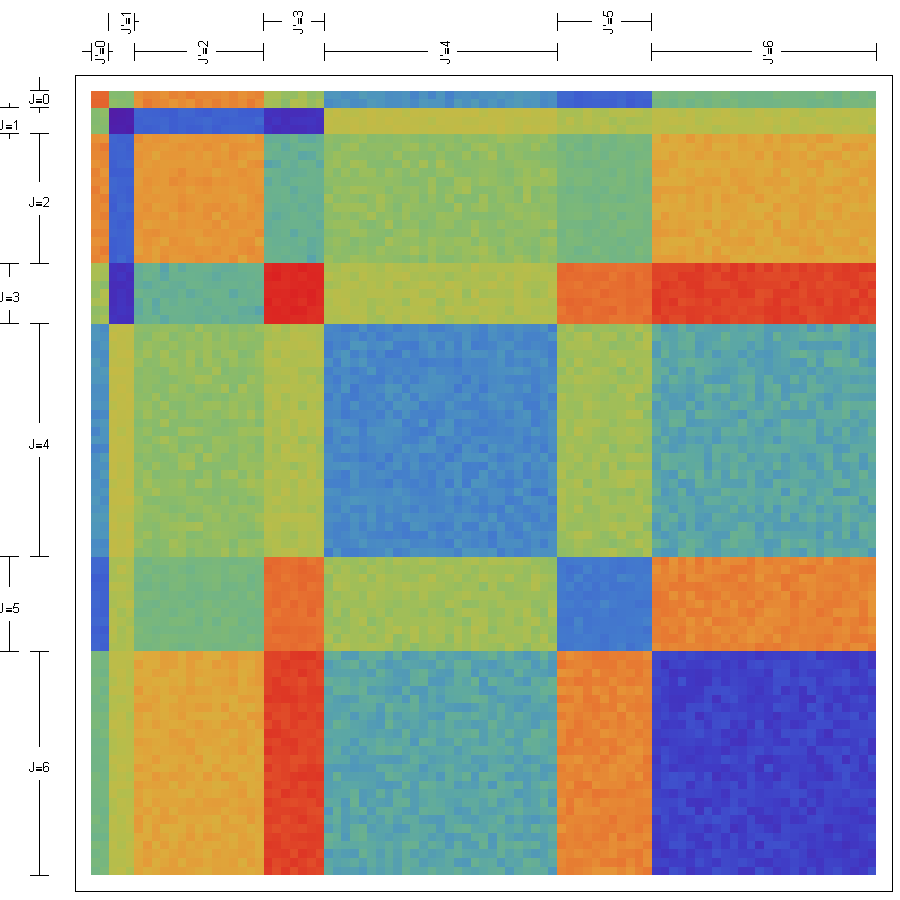
\includegraphics[width=0.85\textwidth]{./figures/blockStruct.pdf}
	\caption{The J-J' block structure for $\underbar{\text{f}}^2$}
	\label{JJ blocks} 
\end{figure}

In \qlanth these blocks are put together by the function \codetext{JJBlockMatrix} which adds together the contributions from the different terms in the Hamiltonian.

\lstinputlisting[language=Mathematica]{./fundefs/JJBlockMatrix.tex}

Once these blocks have been calculated and saved to disk (in the folder \codetext{./hams/}) the function \codetext{HamMatrixAssembly} takes them, assembles the arrays in block form, and finally flattens them to provide a sparse rank-2 array. These are the arrays that are finally diagonalized to find energies and eigenstates. Through options, this function can also return the Hamiltonian in block form, which is useful for the level description of the eigenstates.

\lstinputlisting[language=Mathematica]{./fundefs/HamMatrixAssembly.tex}

In \qlanth the reduced matrix elements of all operators, and the subsequent matrix elements of $\ham$ are calculated exactly. This is in contrast to what is done in older alternatives to \qlanth such as \codetext{linuxemp}, in which calculations of reduced matrix elements were obtained from tables calculated with finite precision. To underscore this fact, \eqnref{eqn:block-example} shows an example of a J-J block as contained in \qlanth.

\begin{sidewaystable}
	\begin{equation}
		\begin{array}{|c|c|c|c|}
		\hline
		  & & & \\
		& \ket{\LSJMstate{4}{F}{1}{-1}} & \ket{\LSJMstate{4}{F}{1}{0}} & \ket{\LSJMstate{4}{F}{1}{1}} \\
		  & & & \\
		\hline
		  & & & \\
		 \bra{\LSJMstate{4}{F}{1}{-1}} &
		 \makecell[c]{
		 	2 \alpha 
		 	+\beta 
		 	-\frac{\Bkq{2}{0}}{10}
		 	+\gamma \\
		 	-\frac{\zeta }{2}
		 	+\frac{14\Fk{0}}{13}
		 	+\frac{43 \Fk{2}}{195}
		 	+\frac{19 \Fk{4}}{429} \\
		 	-\frac{875\Fk{6}}{5577}
		 	+2 \Mk{0} \sigma_\text{SS}
		 	+\frac{61 \Mk{0}}{12} \\
		 	+4 \Mk{2}\sigma_\text{SS} 
		 	+\frac{145 \Mk{2}}{12} 
		 	+\frac{50 \Mk{4} \sigma_\text{SS}}{11} \\
		 	+\frac{1805 \Mk{4}}{132}
		 	+\frac{43 \Pk{2}}{1080} 
		 	+\frac{19\Pk{4}}{2376} \\
		 	-\frac{875\Pk{6}}{30888}
		   } &
		   -\frac{\sqrt{3}
		   \Bkq{2}{1}}{10}-\frac{1}{10} i \sqrt{3} \Skq{2}{2} &
		   -\frac{1}{5} \sqrt{\frac{3}{2}}\Bkq{2}{2}-\frac{1}{5} i \sqrt{\frac{3}{2}} \Skq{2}{2} \\
		   & & & \\
		   \hline
		   & & & \\
		 \bra{\LSJMstate{4}{F}{1}{0}} &
		 -\frac{\sqrt{3} \Bkq{2}{1}}{10}+\frac{1}{10} i \sqrt{3} \Skq{2}{2} &
		 \makecell[c]{
		 	2 \alpha 
		 	+\beta 
		 	+\frac{\Bkq{2}{0}}{5}
		 	+\gamma \\
		 	-\frac{\zeta }{2}
		 	+\frac{14 \Fk{0}}{13}
		 	+\frac{43\Fk{2}}{195}
		 	+\frac{19 \Fk{4}}{429} \\
		 	-\frac{875 \Fk{6}}{5577}
		 	+2 \Mk{0}\sigma_\text{SS}
		 	+\frac{61 \Mk{0}}{12} \\
		 	+4\Mk{2} \sigma_\text{SS} 
		 	+\frac{145\Mk{2}}{12}
		 	+\frac{50 \Mk{4} \sigma_\text{SS}}{11} \\
		 	+\frac{1805\Mk{4}}{132}
		 	+\frac{43 \Pk{2}}{1080}
		 	+\frac{19 \Pk{4}}{2376} \\
		 	-\frac{875\Pk{6}}{30888}
		   } &
		   \frac{\sqrt{3} \Bkq{2}{1}}{10}+\frac{1}{10} i \sqrt{3} \Skq{2}{2}
		   \\
		   & & & \\
		   \hline
		   & & & \\
		\bra{\LSJMstate{4}{F}{1}{1}} &
		 	-\frac{1}{5} \sqrt{\frac{3}{2}} \Bkq{2}{2}
		 	+\frac{1}{5} i \sqrt{\frac{3}{2}} \Skq{2}{2} &
		   \frac{\sqrt{3} \Bkq{2}{1}}{10}
		   -\frac{1}{10} i \sqrt{3} \Skq{2}{2} & 
		   \makecell[c]{
		   2 \alpha 
		   +\beta
		   -\frac{\Bkq{2}{0}}{10}
		   +\gamma \\
		   -\frac{\zeta }{2}
		   +\frac{14 \Fk{0}}{13}
		   +\frac{43\Fk{2}}{195}
		   +\frac{19 \Fk{4}}{429} \\
		   -\frac{875 \Fk{6}}{5577}
		   +2 \Mk{0}\sigma_\text{SS}
		   +\frac{61 \Mk{0}}{12} \\
		   +4 \Mk{2} \sigma_\text{SS}
		   +\frac{145\Mk{2}}{12}
		   +\frac{50 \Mk{4} \sigma_\text{SS}}{11} \\
		   +\frac{1805\Mk{4}}{132}
		   +\frac{43 \Pk{2}}{1080}
		   +\frac{19 \Pk{4}}{2376} \\
		   -\frac{875\Pk{6}}{30888}
		   } \\
		   & & & \\
		   \hline
		\end{array}
	\end{equation}
	\label{eqn:block-example}
\end{sidewaystable}


\subsection{Kramers' degeneracy}

In the odd-electron cases, every energy is at least doubly degenerate. In \qlanth, except in the case of the experimental data compiled for \LaFthree, Kramers' degeneracy is given/expected explicitly.

\section{Interactions}\label{section:interactions}

\subsection{$\hamKineticSymbol$: kinetic energy}

    \begin{equation}
        \hamKineticSymbol = -\frac{\hbar^2}{2m}\sum_{i=1}^N \nabla_i^2 \text{ (kinetic energy of N v-electrons)}
    \end{equation}

    Since our description is limited to a single configuration, the kinetic energy simply contributes a constant energy shift, and since all we care about are energy differences, then this term can be omitted from the analysis.
    
    To interpret the range of energies that result from diagonalizing the \hamilton, it might be instructive, however, to note that this term imparts an energy of about $10\,\eV \approx 10^6 \Kayser$\footnote{Note, $\text{(Kayser) }\Kayser \equiv \invcm$, see section on units.} to each electron.

\subsection{$\hamNuclearCoulombSymbol$: the central field potential}

\begin{equation}
\hamNuclearCoulombSymbol = -e^2 \sum_{i=1}^{Z} \frac{1}{r_{i}} + e^2 \underbracket{\sum_{i=1}^{\numE}\sum_{j=1}^{Z-\numE} \frac{1}{r_{ij}}}_{\substack{
        \text{Repulsion be-} \\
        \text{tween valence} \\
        \text{and inner shell} \\
        \text{electrons} 
        }
      } \approx \sum_{i=1}^\numE V_\text{sn}(r_i) \text{ (with Z = atomic No.)}
\end{equation}


In principle, the sum over the Coulomb potential should extend over the nuclear charge and over all the electrons in the atom (not just the valence electrons). However, given the shell structure of the atom, the lanthanide ions ``see'' the nuclear charge as shielded by a xenon core. Since every closed shell is a singlet, having spherical symmetry, these shields are like spherical shells surrounding the nucleus.

	The precise form of $V_\text{sn}(r_i)$ is not of our concern here; all that matters is that we assume that it is spherically symmetric so that we can justify the separation of radial and angular parts of the wavefunctions.

\subsection{$\hamCoulombEESymbol$: e:e repulsion}
 
    \begin{equation}
        \hamCoulombEESymbol = \hamCoulombEE = \sum_{k=0,1,2,3} \Ek{k} \ek{k}
    \end{equation}  

    This term is the first we will not discard. Calculating this term for the \fn configurations was one of the contributions from Slater, as such the parameters we use to write it up are called \textit{Slater integrals}. After the analysis from Slater, Giulio Racah contributed further to the analysis of this term \cite{racah_theory_1949}. The insight that Racah had was that if in a given operator one identifies the parts in it that transform accordingly to the different symmetry groups present in the problem, then calculating the necessary matrix element in all \fn configurations can be greatly simplified.

    The functions used in \ql to compute these LS-reduced matrix elements \footnote{An LS-reduced matrix element is ...} are \codetext{Electrostatic} and \codetext{fsubk}. In addition to these, the LS-reduced matrix elements of the tensor operators $\op{C}^{(k)}$ and $\op{U}^{(k)}$ are also needed. These functions are based in equations 12.16 and 12.17 from \cite{cowan_theory_1981} as specialized for the case of electrons belonging to a single \fn configuration. By default this term is computed in terms of $\Fk{k}$ Slater integrals, but it can also be computed in terms of the $\Ek{k}$ Racah parameters, the functions \codetext{EtoF} and \codetext{FtoE} are useful for going from one representation to the other.
    
    \begin{equation}
    \redbraopket{\forb^n\alpha\LSterm{2S+1}{L}}
        {\hamCoulombEESymbol}
        {\forb^n\alpha'\LSterm{2S'+1}{L'}} = \sum_{k=0,2,4,6} \Fk f_k(n,\alpha{LS},\alpha'{L'S'})
    \end{equation} 
    where
    \begin{multline}
        f_k(n,\alpha{LS},\alpha'{L'S'}) = \frac{1}{2} 
            \kronecker{S}{S'}
            \kronecker{L}{L'}
            \redbraopket{\forb}
                {\op{\mathcal{C}}^{(k)}}
                {\forb}^2 \times \\
            \left\{ 
                \frac{1}{\tpo{L}} \sum_{\alpha''L''} 
                    \redbraopket{\forb^\numE \alpha'' L'' S}
                        {\op{U}^{(k)}}
                        {\forb^\numE \alpha L S} 
                \redbraopket{\forb^\numE \alpha'' L'' S}
                    {\op{U}^{(k)}} 
                    {\forb^\numE \alpha' L S}
                - \kronecker{\alpha}{\alpha'}
                    \frac{\numE \left(4 \forb + 2 - \numE\right)}
                        {(\tpo{\forb})(4 \forb + 1)} 
            \right\}.
    \end{multline}       

	\foreach \name in {Electrostatic, fsubk, EtoF, FtoE}{ 
	        \lstinputlisting[language=Mathematica]{./fundefs/\name.tex}
	    }

\subsection{$\hamSpinOrbitSymbol$: spin-orbit}

	The spin-orbit interaction arises from the interaction of the magnetic moment of the electron and the magnetic field that its orbital motion generates. In terms of the central potential $V_{\text{s:n}}$, the spin-orbit term for a single electron is
    \begin{equation}
        \op{\mathcal{h}}_{\text{s:o}} = \frac{\hbar^2}{2\me^2 c^2} \left(\frac{1}{r}\frac{\mathrm{d}V_{\text{s:n}}}{\mathrm{d}r}\right)\op{l}\cdot{\op{s}} \DEF \zeta{(r)} \op{l}\cdot\op{s}.
    \end{equation}
    Adding this term for all the $\numE$ valence electrons, and replacing $\zeta(r)$ by its radial average $\spinZeta$ then gives
    \begin{equation}
    \hamSpinOrbitSymbol = \spinZeta \sum_i^{\numE} \dotp{\op{l}_i}{\op{s}_i}.
    \end{equation}

    From equations 2-106 to 2-109 in Wybourne \cite{wybourne_electrostatic_1963} the matrix elements we need are given by
    \begin{multline} 
        \braopket{\alpha LSJ \Msub{J} }{\hamSpinOrbitSymbol}{\alpha' L'S'J'\Msub{J'}} = 
        \spinZeta
        \kronecker{J}{J'}
        \kronecker{\Msub{J}}{\Msub{J'}}
        \braopket{\alpha LSJ \Msub{J} }{\sum_i^{\numE} \dotp{\op{l}_i}{\op{s}_i}}{\alpha' L'S'J\Msub{J}} \\ 
        = \spinZeta \kronecker{J}{J'}
        \kronecker{\Msub{J}}{\Msub{J'}} \phaser{J+L+S'} 
            \sixj{L}{L'}{1}{S'}{S}{J} 
            \braopket{\alpha LS}{\sum_i^{\numE} \dotp{\op{l}_i}{\op{s}_i}}{\alpha' L'S'} \\
        = \spinZeta \kronecker{J}{J'}
        \kronecker{\Msub{J}}{\Msub{J'}} \phaser{J+L+S'} 
            \sixj{L}{L'}{1}{S'}{S}{J} 
            \sqrt{\lorb (\lorb + 1)(2\lorb + 1)} 
            \redbraopket{\alpha{LS}}{\op{V}^{(11)}}{\alpha'L'S'},
    \end{multline}
where $\op{V}^{(11)}$ is a double tensor operator of rank one over spin and orbital parts defined as 
    \begin{equation}
        \op{V}^{(11)} = \sum_{i=1}^\numE \left( \op{s}\op{u}^{(1)} \right)_i,
    \end{equation}
    in which the rank on the spin operator $\op{s}$ has been omitted, and the rank of the orbital tensor operator given explicitly as 1.

    In \qlanth the reduced matrix elements for this double tensor operator are calculated by \codetext{ReducedV1k} and stored in a static association called \codetext{ReducedV1kTable}. The reduced matrix elements of this operator are calculated using equation 2-101 from Wybourne \cite{wybourne_spectroscopic_1965}:
    \begin{multline} 
        \redbraopket{\lorb^\numE \psi}{\op{V}^{(1k)}}{\lorb^\numE \psi'} = 
            \redbraopket{\lorb^\numE \alpha L S}
                {\op{V}^{(1k)}}
                {\lorb^\numE \alpha'L'S'} =
            \numE 
                \sqrt{\sspin (\sspin + 1) (2\sspin + 1)}
                \sqrt{\tpobraket{S}\tpobraket{L}\tpobraket{S'}\tpobraket{L'}} \times \\
        \sum_{\bar{\psi}}
            \phaser{\bar{S} + \bar{L} + S + L + \lorb + \sspin + k + 1}
            \cfpinv{\psi}{\bar{\psi}}
            \cfp{\bar{\psi}}{\psi'}
            \sixj{S}     {S'}     {1}
                {\sspin} {\sspin} {\bar{S}}
            \sixj{L}     {L'}    {k}
                {\lorb} {\lorb} {\bar{L}}
    \label{eqn:reducedV1k}
    \end{multline}
    In this expression the sum over $\bar{\psi}$ depends on $(\psi,\psi')$ and is over all the states in $\lorb^{n-1}$ which are common parents to both $\psi$ and $\psi'$. Also note that in the equation above, since our concern are $\forb$-electron configurations, we have $\lorb = 3$ and $\sspin = \frac{1}{2}$.

\foreach \name in {ReducedV1k}{ 
        \lstinputlisting[language=Mathematica]{./fundefs/\name.tex}
    }
 
	These reduced matrix elements are then used by the function \codetext{SpinOrbit}.

\foreach \name in {SpinOrbit}{ 
        \lstinputlisting[language=Mathematica]{./fundefs/\name.tex}
    } 
 
\subsection{$\hamTreesSymbol, \hamGTwoSymbol, \hamSOSevenSymbol$: electrostatic configuration interaction}

    These are the first terms where we take into account the contributions from \confint. Rajnak and Wybourne \cite{rajnak_configuration_1963} showed that \confint of the electrostatic interactions corresponding to two-electron excitations from $\forb^\numE$  can be represented through the Casimir operators of the groups $\SO{3}$, $\Gtwo$, and $\SO{7}$. This borrowed from an earlier insight of Trees \cite{trees_l_1952}, who realized that an addition of a term proportional to $L(L+1)$ improved the energy calculations for the second spectrum of manganese (Mn-II) and the third spectrum of iron (Fe-III).

    One of these Casimir operators is the familiar $\op{L}^2$ from $\SO{3}$. In analogy to $\op{L}^2$ in which the quantum number $L$ can be used to determine the eigenvalues, in the cases of $\hamGTwoSymbol$ the necessary state label is the $U$ label of the $LS$ term, and in the case of $\hamSOSevenSymbol$ the necessary label is $W$. If $\Lambda_{\Gtwo}\!(U)$ is used to note the eigenvalue of the Casimir operator of $\Gtwo$ corresponding to label $U$, and $\Lambda_{\SO{7}}\!(W)$ the eigenvalue corresponding to state label $W$, then the matrix elements of $\hamTreesSymbol$, $\hamGTwoSymbol$ and $\hamSOSevenSymbol$ are diagonal in all quantum numbers (see Rajnak and Wybourne \cite{rajnak_configuration_1963}) and are given by
    \begin{align}
        \braopket{\lorb^\numE \alpha S L J \Msub{J}}
            {\hamTreesSymbol}
            {\lorb^\numE \alpha' S' L' J' \Msub{J}'} &=
            \casimirAlpha
            \kronecker{\alpha{SLJ}\Msub{J}}{\alpha'{S'L'J'}\Msub{J}'}
            L(L+1) \\
        \braopket{\lorb^\numE U \alpha S L J \Msub{J}}
            {\hamGTwoSymbol}
            {\lorb^\numE U \alpha' S' L' J' \Msub{J}'} &=
            \casimirBeta
            \kronecker{\alpha{SLJ}\Msub{J}}{\alpha'{S'L'J'}\Msub{J}'}
            \Lambda_{\Gtwo}\!(U) \\
        \braopket{\lorb^\numE W \alpha S L J \Msub{J}}
            {\hamSOSevenSymbol}
            {\lorb^\numE W \alpha' S' L' J' \Msub{J}} &=
            \casimirGamma
            \kronecker{\alpha{SLJ}\Msub{J}}{\alpha'{S'L'J'}\Msub{J}'}
            \Lambda_{\SO{7}}\!(W)
    \end{align}
    In \qlanth the role of $\Lambda_{\SO{7}}\!(W)$ is played by the function \codetext{GSO7W}, the role of $\Lambda_{\Gtwo}\!(U)$ by \codetext{GG2U}, and the role of  $\Lambda_{\SO{3}}\!(L)$ by \codetext{CasimirSO3}. These are used by \codetext{CasimirG2}, \codetext{CasimirSO3}, and \codetext{CasimirSO7} which find the corresponding ${U,W,L}$ labels to the $LS$ terms provided to them. Finally, the function \codetext{ElectrostaticConfigInteraction} puts them together.

    \foreach \name in {ElectrostaticConfigInteraction}{
        \lstinputlisting[language=Mathematica]{./fundefs/\name.tex}
    }

\subsection{$\hamSpinSpinSpinOtherOrbitSymbol$: \spinspin and \soo}\label{subsection:ss-soo}


	The calculation of the $\hamSpinSpinSpinOtherOrbitSymbol$ is qualitatively different from the previous ones. The previous ones were self-contained in the sense that the reduced matrix elements that we require we also computed on our own. 
	\begin{wrapfigure}{r}{0.3\textwidth}
\centering
	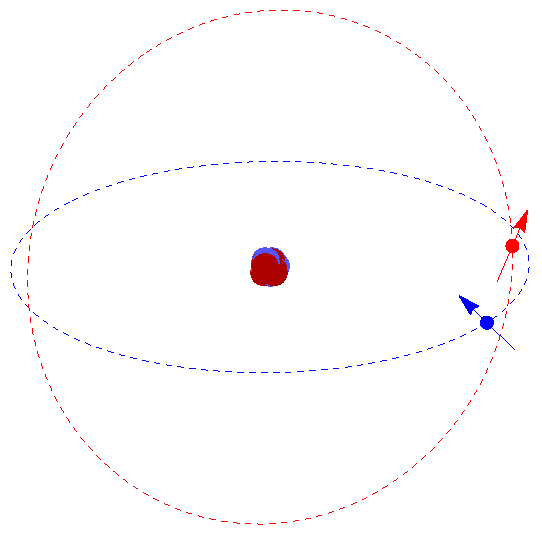
\includegraphics[width=0.3\textwidth]{./figures/ss-soo.pdf}
\end{wrapfigure}
	In the case of the interactions that follow from here, we use values from literature for reduced matrix elements either in $\forb^2$ or in $\forb^3$ and then we ``pull'' them up for all $\forb^{\numE}$ configurations with help of the \cfps.



    The analysis of \soo, and the \spinspin contributions used in  \qlanth is that of Judd, Crosswhite, and Crosswhite \cite{judd_intra-atomic_1968}. Much as the spin-orbit effect can be extracted from the Dirac equation as a relativistic correction, the multi-electron spin-orbit effects can be derived from the Breit operator $\ham_B$  \cite{bethe_quantum_1957} which is a term added to the relativistic description of a many-particle system in order to account for retardation of the electromagnetic field
    \begin{equation}
    \ham_B = -\frac{1}{2}e^2 \sum_{i>j} \left[ \left(\alpha_i\cdot\alpha_j\right)\frac{1}{r_{ij}} + \left(\alpha_i\cdot{\vec{r}_{ij}}\right)\left(\alpha_j\cdot\vec{r}_{ij}\right) \frac{1}{r_{ij}^3} \right].
    \end{equation}
    When this operator is expanded in powers of $v/c$, a number of non-relativistic inter-electron interactions result. Two of them are the \soo and \spinspin interactions.
    As usual, the radial part of the Hamiltonian is averaged, which in this case gives appearance to the Marvin integrals \index{Marvin integrals}
    \begin{equation} 
    \Mk{k} \DEF \frac{e^2\hbar^2}{8m^2c^2} \braopket{(nl)^2}{\frac{r_<^k}{r_>^{k+3}}}{(nl)^2}.
    \end{equation}
    \index{spin-spin} With these, the expression for the \spinspin term within the single configuration description is \cite{judd_intra-atomic_1968}
    \begin{multline}
    \ham_{s:s} = -2 \sum_{i\neq{j}}
        \sum_k \Mk{k}
            \sqrt{(k+1)(k+2)(2k+3)} 
            \redbraopket{\lorb}{\Ck{k}}{\lorb} 
            \redbraopket{\lorb}{\Ck{k+2}}{\lorb}
            \left\{
                \wdouble{i}{1}{k}
                \wdouble{j}{1}{k+2}
            \right\}^{(2,2)0}
    \end{multline}
    and the one for \soo \index{spin-other-orbit}
    \begin{multline}
        \ham_{s:oo} = \sum_{i\neq{j}} 
            \sum_k 
                \sqrt{(k+1)(2\lorb+k+2)(2\lorb-k)}  \times \\ 
        \left[ \left\{ \wdouble{i}{0}{k+1} \wdouble{j}{1}{k} \right\}^{(11)0} 
        \left\{ \Mk{k-1}
            \redbraopket{\lorb}
                {\Ck{k+1}}
                {\lorb}^2
            +
            2 \Mk{k} \redbraopket{\lorb}{\Ck{k}}{\lorb}^2
        \right\} + \right. \\
        \left.
            \left\{ \wdouble{i}{0}{k}\wdouble{j}{1}{k+1} \right\}^{(11)0} 
                \left\{ \Mk{k} 
                    \redbraopket{\lorb}{\Ck{k}}{\lorb}^2
                    + 2 \Mk{k-1}
                    \redbraopket{\lorb}{\Ck{k+1}}{\lorb}^2
                \right\}
        \right].
    \end{multline} 

    In the expressions above $\wdouble{i}{\kappa}{k}$ is a double tensor operator of rank $\kappa$ over spin, of rank $k$ over orbit, and acting on electron $i$. It is defined by its reduced matrix elements as
    \begin{equation} 
    \redbraopket{\lorb}
        {\wdouble{}{\kappa}{k}}
        {\lorb}
        = \sqrt{\tpobraket{\kappa}
            \tpobraket{k}
        }.
    \end{equation} 

    The explicit complexity of the above expressions can be somewhat reduced by identifying them with the scalar part of two new double tensors $\Txyz{1}{1}{0}$ and $\Txyz{2}{2}{0}$ such that
    \begin{align}
    \sqrt{5}\Txyz{2}{2}{0} &\DEF \hamSpinSpinSymbol \\
    -\sqrt{3}\Txyz{1}{1}{0} &\DEF \hamSpinOtherOrbitSymbol.
    \end{align}
    In terms of which the reduced matrix elements in the $\LSJbasis$ basis can be obtained by
    \begin{equation}
        \braopket{\gamma{SLJ}}{\ham}{\gamma'{S'L'J'}} = \kronecker{J}{J'} \sixj{S'}{L'}{J}{L}{S}{t} \redbraopket{\gamma{SL}}{\Txyz{t}{t}{}}{\gamma'{S'L'}}.
    \label{SLtoSLJ for Ttt}
    \end{equation}

    This above relationship is the one effectively used in \qlanth in the functions \codetext{SpinSpin} and \codetext{SOOandECSO}.

    \foreach \name in {SpinSpin, SOOandECSO}{
        \lstinputlisting[language=Mathematica]{./fundefs/\name.tex}
    }

    For two-electron operators such as these, the matrix elements in $\forb^\numE$ are related to those in $\forb^{\numE-1}$ by equation 4 in Judd \etal \cite{judd_intra-atomic_1968}
    \begin{multline}
        \redbraopket{\forb^\numE\psi}
        	{\Txyz{t}{t}{}}
        	{\forb^\numE\psi'} 
        = \frac{\numE}{\numE-2} 
        \sum_{\bar{\psi},\bar{\psi}'}
        \phaser{\bar{S}+\bar{L}+\sspin+\lorb+S'+L'}
        \sqrt{\tpobraket{S}\tpobraket{S'}\tpobraket{L}\tpobraket{L'}} \times \\
        \cfpinv{\psi}{\bar{\psi}}
        \cfpinv{\psi'}{\bar{\psi}'} 
        \sixj{S}{t}{S'}{\bar{S}'}{\sspin}{\bar{S}}
        \sixj{L}{t}{L'}{\bar{L}'}{\lorb}{\bar{L}}
        \redbraopket{\forb^{\numE-1}\bar{\psi}}
        {\Txyz{t}{t}{}}{\forb^{\numE-1}]\bar{\psi}'},
    \label{double cfp escalator}
    \end{multline}
    where the sum runs over the terms $\bar{\psi}$ and $\bar{\psi}'$ in $\forb^{\numE-1}$ which are parents common to $\psi$ and $\psi'$. Using these the matrix elements of $\Txyz{1}{1}{}$ and $\Txyz{2}{2}{}$ in $\forb^2$ can be used to compute all the reduced matrix elements in  $\forb^\numE$. These could then be used together with \eqnref{SLtoSLJ for Ttt} to obtain the matrix elements of $\hamSpinSpinSymbol$ and $\hamSpinOtherOrbitSymbol$. This is done for $\hamSpinSpinSymbol$, but not for $\hamSpinOtherOrbitSymbol$, because this term is traditionally computed (with a slight modification) at the same time as the electrostically-correlated-spin-orbit (see next section).

    These equations are implemented in \qlanth through the following functions: \codetext{Generate{\-}T22{\-}Table}, \codetext{ReducedT22infn}, \codetext{ReducedT22inf2}, \codetext{ReducedT11inf2}. Where \codetext{ReducedT22inf2} and \codetext{ReducedT11inf2} provide the reduced matrix elements for $\Txyz{1}{1}{}$ and $\Txyz{2}{2}{}$ in $\forb^2$ as provided in table II of \cite{judd_intra-atomic_1968}.

    \foreach \name in {GenerateT22Table, ReducedT22infn, ReducedT22inf2, ReducedT11inf2}{
        \lstinputlisting[language=Mathematica]{./fundefs/\name.tex}
    }

\subsection{$\hamECSOSymbol$: \ecso}

    In the same paper \cite{judd_intra-atomic_1968} that describes the \spinspin and \soo interactions, consideration is also given to the emergence of additional corrections due to configuration interaction as described by the following operator (which is what results from the application of perturbation theory to \textit{second} order) (page.  134 of \cite{judd_intra-atomic_1968})
    \begin{equation}
        \ham_{\text{ci}} = -\sum_\chi \sum_i \frac{1}{E_\chi}\xi(r_i) 
            \left(  
                \op{\sspin}_i\cdot\op{\lorb}_i
            \right) \ket{\chi} \bra{\chi} \CoulombNonCentral
            - \frac{1}{E_\chi}\CoulombNonCentral \ket{\chi}\bra{\chi} \xi(r_i) 
                \left( 
                    \op{\sspin}_i\cdot\op{\lorb}_i
                \right) 
    \end{equation} 
    where $\xi(r_h) (\op{\sspin}_h\cdot\op{\lorb}_h)$ is the customary spin-orbit interaction, $E_\chi$ is the energy of state $\ket{\chi}$, $i$ is a label for the valence electrons, $\CoulombNonCentral$ stands for the Coulomb interaction, and $\ket{\chi}$ are states in the configurations with which one is ``interacting''. Since this term includes both the electrostatic term and the spin-orbit one, this is called the \ecso interaction.

    This operator can be identified with the scalar component of a double tensor operator of rank 1 both for the spin and orbital parts of the wavefunction
    \begin{equation}
        \ham_{\text{ci}} = - \sqrt{3}\,\txyz{1}{1}{0}.
    \end{equation}

    Judd \etal \cite{judd_intra-atomic_1968} then go on to list the reduced matrix elements of this operator in the $\forb^2$ configuration. When this is done the Marvin integrals $\Mk{k}$ appear again, but a second set of parameters, the \textit{pseudo-magnetic} parameters $\Pk{k}$, is also necessary \index{Pk} \index{Pseudo-magnetic parameters} \index{Mk} \index{Marvin integrals}
    \begin{equation}
        \Pk{k} = 6 \sum_{f'}
            \frac{\zeta_{ff'}}
                {E_{ff'}}
                R^{(k)}(ff,ff') \text{ for }k=0,2,4,6.
    \end{equation}
    Where $f$ stands for an $\forb$-electron radial eigenfunction, and $f'$ similarly but for a configuration different from $\forb^\numE$. And where
    \begin{align}
        \zeta_{ff'} &\DEF \braopket{f}{\xi(r)}{f'} \\
        R^{(k)}(ff,ff') &\DEF e^2 \braopket{f_1f_2}{\frac{r_<^k}{r_>^{k+1}}}{f_1f_2'}.
    \end{align}
    
In the semi-empirical approach embodied by $\qlanth$, calculating these quantities \textit{ab-initio} is not the objective, they are instead to be defined from experiments. Nonetheless, not only these expressions give theoretical justification to the model, but they also serve to justify the ratios between different orders of these quantities, their relative importance, or their sign. Consequently, both the set of three $\Mk{k}$ and the set of $\Pk{k}$ ultimately rely on a single free parameter each. Such parsimony is desirable given the large number of parameters (about 20) that the Hamiltonian ends up having.

	\index{electrostatically-correlated-spin-orbit}
    Judd \etal further note that $\Pk{0}$ is proportional to the spin orbit operator, and as such its effect is absorbed by the standard spin-orbit parameter $\spinZeta$. They also developed an alternative approach based on group theory arguments. They put together the \soo and the \ecso as a sum of operators $\op{z}_i$ with useful transformation rules 
    \begin{equation}
        \redbraopket{\psi}{\Txyz{1}{1}{} + \txyz{1}{1}{}}{\psi'} = \sum a_i \redbraopket{\psi}{\op{z}_i}{\psi'}.
    \end{equation}

    At this stage a subtle point needs to be raised. As Judd points out, in the sum above, the term $\op{z}_{13}$ that contributes with a tensorial character equal to that of the regular spin-orbit operator. As such, if the goal is obtaining a parametric Hamiltonian that can be fit with uncorrelated parameters, it is then necessary to subtract this part from $\Txyz{1}{1}{} + \txyz{1}{1}{}$. This point was clarified by Chen \etal \cite{chen_few_2008}. Because of this, the final form of the operator contributing both to \soo and the \ecso is
    \begin{equation}
        \hamSpinOtherOrbitSymbol + \hamECSOSymbol = \Txyz{1}{1}{} + \txyz{1}{1}{} - \frac{1}{6}a_{13}\op{z}_{13}
        \label{SOO ECSO sum}
    \end{equation}
    where
    \begin{equation}
        a_{13} = -33 \Mk{0} + 3 \Mk{2} + \frac{15}{11} \Mk{4} - 6 \Pk{0} + \frac{3}{2} \left(\frac{35}{225} \Pk{2} + \frac{77}{1089} \Pk{4} + \frac{25}{1287} \Pk{6}\right).
    \end{equation}

    In \qlanth the contributions from \spinspin, \soo, and \ecso are put together by the function \codetext{MagneticInteractions}. That function queries precomputed values from two associations \codetext{SpinSpinTable} and \codetext{SOOandECSOTable}. In turn these two associations are generated by the functions \codetext{GenerateSpinOrbitTable} and \codetext{GenerateSOOandECSOTable}. Note that both \spinspin and \soo end up contributing through $\Mk{k}$, however there doesn't seem to be consensus about adding them together, as such \qlanth allows including or excluding the \spinspin contribution, this is done with a control parameter $\sigma_{SS}$ (1 for including, 0 for excluding).

    \foreach \name in {MagneticInteractions, GenerateSpinOrbitTable, GenerateSOOandECSOTable}{
        \lstinputlisting[language=Mathematica]{./fundefs/\name.tex}
    }

    The function \codetext{GenerateSpinSpinTable} calls the function \codetext{SpinSpin} over all possible combinations of the arguments $\{\numE, SL, S'L', J\}$. In turn the function \codetext{SpinSpin} queries the precomputed values of the double tensor $\Txyz{2}{2}{}$ which are stored in the association \codetext{T22Table}. 


    \foreach \name in {GenerateSpinSpinTable, SpinSpin}{ 
        \lstinputlisting[language=Mathematica]{./fundefs/\name.tex}
    }

    The association \codetext{T22Table} is computed by the function \codetext{GenerateT22Table}. This function populates \codetext{T22Table} with keys of the form $\{\numE, SL, S'L'\}$. It does this by using the function \codetext{ReducedT22inf2} in the base case of $\forb^2$, and \codetext{ReducedT22infn} for configurations above $\forb^2$. When \codetext{ReducedT22infn} is called, the sum in \eqnref{double cfp escalator} is carried out using $t=2$. When \codetext{ReducedT22inf2} is called, the reduced matrix elements from \cite{judd_intra-atomic_1968} are used. 

    \foreach \name in {GenerateT22Table, ReducedT22infn, ReducedT22inf2}{
        \lstinputlisting[language=Mathematica]{./fundefs/\name.tex}
    }

    The function \codetext{GenerateSOOandECSOTable} calls the function \codetext{SOOandECSO} over all possible combinations of the arguments $\{\numE, SL, S'L', J\}$ and uses their values to populate the association \codetext{SOOandECSOTable}. In turn the function \codetext{SOOandECSO} queries the precomputed values of \eqnref{SOO ECSO sum} as stored in the association \codetext{SOOandECSOLSTable}. 

    \foreach \name in {GenerateSOOandECSOTable, SOOandECSO, SOOandECSO}{
        \lstinputlisting[language=Mathematica]{./fundefs/\name.tex}
    }

    The association \codetext{SOOandECSOLSTable} is computed by the function \codetext{GenerateSOOandECSOLSTable}. This function populates \codetext{SOOandECSOLSTable} with keys of the form $\{\numE, SL, S'L'\}$. It does this by using the function \codetext{ReducedSOOandECSOinf2} in the base case of $\forb^2$, and \codetext{ReducedSOOandECSOinfn} for configurations above $\forb^2$. When \codetext{ReducedSOOandECSOinfn} is called the sum in \eqnref{double cfp escalator} is carried out using $t=1$. When \codetext{ReducedSOOandECSOinf2} is called the reduced matrix elements from \cite{judd_intra-atomic_1968} are used.

    \foreach \name in {ReducedSOOandECSOinfn, ReducedSOOandECSOinf2}{
        \lstinputlisting[language=Mathematica]{./fundefs/\name.tex}
    }

\subsection[$\ham_3$: three-body effective operators]{$\ham_{\trispoke}$: three-body effective operators}\label{qlanth:three-body}

\index{Tk} \index{three-body effective operators}

The three-body operators in the \hamilton are due to the \confint effects of the Coulomb repulsion. More specifically, they originate from configuration interaction between the ground configuration $(4\forb)^{\numE}$ and single electron excitations to the $(4\forb)^{\numE\pm{1}}(n'\lorb')^{\mp{1}}$ configurations.

The operators that can be used to span the resulting effects were initially studied by Wybourne and Rajnak in 1963 \cite{rajnak_configuration_1963}, their analysis was complemented soon after by Judd \cite{judd_three-particle_1966}, and revisited again by Judd in 1984 \cite{judd_complete_1984}.

This model interaction is spanned by a set of 14 $\op{t}_i$ of operators ($\op{t}$ from \textit{t}hree)
\begin{equation}
\ham_{\trispoke} = {\paramcolor{T'^{(2)}}}\tk{2}' + {\paramcolor{T'^{(11)}}}\tk{11}' \hamEffectiveThreeBody, 
\end{equation}
where $\tk{2}$ and $\tk{11}$ are operators that have orthogonal alternatives represented by $\tk{2}'$ and $\tk{11}'$ (see \cite{judd_complete_1984}). \qlanth includes the legacy operator $\tk{2}$ since it was used for important work during and before the 1980s.

The omission of some indices in this sum has to do with the fact that the way in which these are defined in terms of their index (see \cite{judd_three-particle_1966}) gives rise to two-body operators which can be absorbed by the two-body terms in the Hamiltonian. As such, it is not so much that they are not included, but rather that their effects are considered to be accounted for elsewhere. This is representative of a common feature of configuration interaction: it gives rise to new intra-configuration operators, but it also contributes to already present operators; this makes it harder to approximate the model parameters \textit{ab-initio}, but is not a practical obstacle for the semi-empirical approach (although it certainly complicates the physical interpretation that each parameter has). Furthermore, it is often the case that the operator set is limited to the subset \{2,3,4,6,7,8\}; a practice that is justified \textit{post-facto} after seeing that these are sufficient to describe the data.

The calculation of a three body operator matrix elements across the $\forb^{\numE}$ configurations is analogous to how a two-body operator is calculated. Except that in this case what is needed are the reduced matrix elements in $\forb^3$ and the equation that is used to propagate these across the other configurations is equation 4 of \cite{judd_three-particle_1966} (here adding the explicit dependence on $J$ and $\Msub{J}$):
\begin{equation} 
	\braopket{\forb^{\numE}\psi}
		{\op{t}_i}
		{\forb^{\numE}\psi'} =
		\kronecker{J}{J'}
		\kronecker{\Msub{J}}{\Msub{J}'} 
		\frac{\numE}{\numE-3} 
		\sum_{\bar{\psi}\bar{\psi}'}
			\cfpinv{\psi}{\bar{\psi}}
        	\cfpinv{\psi'}{\bar{\psi}'}
        	\braopket{\forb^{\numE-1}\bar{\psi}}{\op{t}_i}{\forb^{\numE-1}\bar{\psi}'}.
\label{eqn:three body escalator}
\end{equation}
The sum in this expression runs over the parents in $\forb^{\numE-1}$ that are common to both the daughter terms $\psi$ and $\psi'$ in $\forb^{\numE}$. The equation above yielding LSJMJ matrix elements, and being diagonal in $J$, $\Msub{J}$ as is due to a scalar operator.

In \qlanth this is all implemented in the function \codetext{GenerateThreeBodyTables}. Where the matrix elements in $\forb^3$ are from \cite{judd_complete_1984}, where the data has been digitized in the files \codetext{Judd1984-1.csv} and \codetext{Judd1984-2.csv}, which are parsed through the function \codetext{ParseJudd1984}.
 
 In \codetext{GenerateThreeBodyTables} a special case is made for $\tk{2}$ and $\tk{11}$ which are calculated differently beyond the half-filled shell. In the case of the other $\tk{k}$ operators, beyond $\forb^7$ the matrix elements simply see a global sign flip, whereas in the case of $\tk{2}$ and $\tk{11}$ the \cfps beyond $\forb^7$ are used. This yields the unexpected result that in the $\forb^{12}$ configuration, which corresponds to two holes, there is a non-zero three body operator $\tk{2}$. This is an arcane result that was corrected by Judd in 1984 \cite{judd_complete_1984}, but which lingered long enough that important work in the 1980s was calculated with it. When calculations are carried out, if $\tk{2}'/\tk{11}'$ is used then $\tk{2}/\tk{11}$ should not be used and vice versa.
 
 One additional feature of $\tk{2}$ that needs to be accounted for, is that it doesn't have the simple relationship for conjugate configurations that all the other $\op{t}_i$ operators have. For the sake of simplicity, and to avoid having to explicitly store matrix elements beyond $\forb^7$ \qlanth takes the approach of adding a control parameter \codetext{t2Switch} which needs to be set to 1 if below or at $\forb^7$ and set to 0 if above $\forb^7$. \index{t2Switch}
 
 \foreach \name in {GenerateThreeBodyTables, ParseJudd1984}{ 
        \lstinputlisting[language=Mathematica]{./fundefs/\name.tex}
    }
 
\subsection{$\hamCrystalFieldSymbol$: crystal-field} 
	\index{crystal field}
	The crystal-field partially accounts for the influence of the surrounding lattice on the ion. The simplest picture of this influence imagines the lattice as responsible for an electric field felt at the position of the ion. This electric field corresponding to an electrostatic potential described as a multipolar sum of the form:  
    \begin{equation}   
    V(r_i, \theta_i, \phi_i) = \sum_{k=1}^\infty \sum_{q=-k}^k \Akq r_i^k \Ckq{k}{q}(\theta_i, \phi_i) 
    \end{equation}  
    \index{spherical harmonics}
    where the $\Ckq{k}{q}$ are spherical harmonics normalized with the Racah convention \index{Racah convention}
    \begin{equation}
    		\Ckq{k}{q} = \sqrt{\frac{4\pi}{{2k+1}}} Y^{(k)}_q.
    \end{equation}


    Here we have chosen a coordinate system with its origin at the position of the nucleus, and in which we only have positive powers of the distance $r_i$ because we have expanded the contributions from all the surrounding ions as a sum over spherical harmonics centered at the position of the nucleus, without $r$ ever large enough to reach any of the positions of the lattice ions. 

    Furthermore, since we have $\numE$ valence electrons, then the total crystal field potential is 
    \begin{equation}
        \hamCrystalFieldSymbol(\vec{r}) = 
        	\sum_{i=1}^\numE
        	\sum_{k=0}^\infty
        	\sum_{q=-k}^{k} \Akq r_i^k \Ckq{k}{q}(\theta_i,\phi_i).
    \label{eqn:crystal sum}
    \end{equation}

    And if we average the radial coordinate,
    \begin{equation}
        \hamCrystalFieldSymbol = \sum_{i=1}^\numE \sum_{k=1}^\infty \sum_{q=-k}^{k} \Bcomplexkq{k}{q} {\Ckq{k}{q}}\!(i) 
    \end{equation}
    where the radial average is included as
    \begin{equation}
    \Bcomplexkq{k}{q} \DEF \Akq {\langle 4f | r^k | 4f\rangle}.
    \end{equation}
    
    $\Bcomplexkq{k}{q}$ may be complex in general. However, since the sum in \eqnref{eqn:crystal sum} needs to result in a real and Hermitian operator, there are restrictions on $\Bcomplexkq{k}{q}$ that need to be accounted for. Once the behavior of $\Ckq{k}{q}$ under complex conjugation is considered, $\Ckq{k}{q}{}^* = \phaser{q}\Ckq{k}{-q}$, it is necessary that
    \begin{equation}
    	\Bcomplexkq{k}{q} = \phaser{q}\Bcomplexkq{k}{-q}^{*}.
    \end{equation}
    
    Presently the sum over $q$ spans both its negative and positive values. This can be limited to only the non-negative values of $q$. Separating the real and imaginary parts of $\Bcomplexkq{k}{q}$ such that $\Bcomplexkq{k}{q} = \Bkq{k}{q} + i \Skq{k}{q}$ for $q\neq{0}$ and $\Bcomplexkq{k}{0} = 2\Bkq{k}{0}$ the sum for the crystal field can then be written as
    \begin{equation}
        \hamCrystalFieldSymbol(\vec{r}) = 
        	\sum_{i=1}^\numE
        	\sum_{k=0}^\infty
        	\sum_{q=0}^{k} \Bkq{k}{q} \left(\Ckq{k}{q} + \phaser{q}\Ckq{k}{-q}\right) + i \Skq{k}{q} \left(\Ckq{k}{q} - \phaser{q}\Ckq{k}{-q}\right).
    \label{eqn:better crystal sum}
    \end{equation}
    
    A staple of the Wigner-Racah algebra is writing up operators of interest in terms of standard ones for which the matrix elements are straightforward.  One such operator is the unit tensor operator $\op{u}^{(k)}$ for a single electron. The Wigner-Eckart theorem -- on which all of this algebra is an elaboration -- effectively separates the dynamical and geometrical parts of a given interaction; the unit tensor operators isolate the geometric contributions. This irreducible tensor operator $\op{u}^{(k)}$ is defined as the tensor operator having the following reduced matrix elements (written in terms of the triangular delta, see section on notation):
    \begin{equation}
    \redbraopket{\ell}{\op{u}^{(k)}}{\ell'} = 1.
    \end{equation}

    In terms of this tensor one may then define the symmetric (in the sense that the resulting operator is equitable among all electrons) unit tensor operator for $\numE$ particles as
    \begin{equation}
        \op{U}^{(k)} = \sum_{i}^{\numE} \op{u}^{(k)}_i.
    \end{equation}
    This tensor is relevant to the calculation of the above matrix elements since 
    \begin{equation}
        \Ckq{k}{q} = \redbraopket{\lorb}
                    {\Ck{k}}
                    {\lorb{'}} \op{u}^{(k)}_q 
            = \phaser{\lorb}
            \sqrt{\tpobraket{\lorb}\tpobraket{\lorb{'}}}
            \threej{\lorb}{k}{\lorb'}{0}{0}{0} \op{u}^{(k)}_q.
    \end{equation}
    With this, the matrix elements of $\hamCrystalFieldSymbol$ in the $\LSJMbasis$ basis are: 
    \begin{align}
        \overbracket{\braopket{\lorb^\numE \alpha SLJ \Msub{J}}{\hamCrystalFieldSymbol}{\lorb^\numE \alpha'S L' J' \Msub{J'}}}^{\text{Wybourne eqn. 6-3}} &= \sum_{k=1}^\infty\sum_{q=-k}^k    
        \Bcomplexkq{k}{q} 
            \braopket{\lorb^\numE \alpha SLJ\Msub{J}}
                {\op{U}^{(k)}_q}
                {\lorb^\numE \alpha'SL'J'\Msub{J'}} 
            \redbraopket{\lorb}
                {\op{C}^{(k)}}
                {\lorb} 
    \label{HCFsum}
    \end{align}
    where the matrix elements of $\op{U}^{(k)}_q$ can be resolved with a 3j symbol as
    \begin{align}
        \overbracket{\braopket{\lorb^\numE \alpha S L J \Msub{J}}
            {\op{U}^{(k)}_q}
            {\lorb^\numE \alpha' S' L' J' \Msub{J'}}}^
            {\text{Wybourne eqn. 6-4}}
            &= 
            \phaser{J-\Msub{J}}
            \threej{J}{k}{J'}
                {-\Msub{J}}{q}{\Msub{J'}}
        \redbraopket{\lorb^\numE \alpha S L J}
                {\op{U}^{(k)}}
                {\lorb^\numE \alpha' S' L'}
    \end{align}
    and reduced a second time with the inclusion of a 6j symbol resulting in
    \begin{align}
        \nonumber \overbracket{\redbraopket{\lorb^\numE \alpha S L J}
            {\op{U}^{(k)}}
            {\lorb^\numE \alpha' S' L'}}^
            {\text{Wybourne eqn. 6-5}}
        &= 
        \phaser{S+L+J'+k} 
        \sqrt{\tpobraket{J}\tpobraket{J'}} \times \\
        & \sixj{J}{J'}{k}{L'}{L}{S}
        \redbraopket{\lorb^\numE \alpha S L}
            {\op{U}^{(k)}}
            {\lorb^\numE \alpha' S' L'}.
    \end{align}
    This last reduced matrix element is finally computed by summing over $\bar{\alpha}\bar{L}\bar{S}$ which are the $\forb^{\numE-1}$ parents which are common to $\ket{\alpha L S}$ and $\ket{\alpha' L' S'}$ from the $\forb^{\numE}$ configuration:
    \begin{multline}
    \overbracket{\redbraopket{\lorb^\numE \alpha S L} 
        {\op{U}^{(k)}}
        {\lorb^\numE \alpha' S' L'}}^{\text{Cowan eqn. 11.53}} = \kronecker{S}{S'} \numE \phaser{\lorb + L + k}
            \sqrt{\tpobraket{L}\tpobraket{L'}} \times \\
    \sum_{\bar{\alpha}\bar{L}\bar{S}} 
        \phaser{\bar{L}} \sixj{\lorb}{k}{\lorb}{L}{\bar{L}}{L'}
        \cfpinv{\lorb^\numE \alpha L S}
            {\lorb^{\numE - 1}\bar{\alpha}\bar{L}\bar{S}}
        \cfp{\lorb^{\numE -1}\bar{\alpha}\bar{L}\bar{S}}{\lorb^\numE\alpha'L'S'}.
    \label{eqn:ReducedUk}
    \end{multline}

    From the $\redbraopket{\lorb}{\op{C}^{(k)}}{\lorb}$, and given that we are using $\lorb = \forb = 3$, we can see that by the triangular condition $\tricondition{3,k,3}$ the non-zero contributions only come from $k=0,1,2,3,4,5,6$. An additional selection rule on $k$ comes from considerations of parity. Since both the bra and the ket in $\braopket{\lorb^\numE \alpha SLJ \Msub{J}}{\hamCrystalFieldSymbol}{\lorb^\numE \alpha'S L' J' \Msub{J'}}$ have the same parity, then the overall parity of the braket is determined by the parity of $\Ckq{k}{q}$, and since the parity of $\Ckq{k}{q}$ is $\phaser{k}$ then for the braket to be non-zero we require that $k$ should also be even. In view of this, in all the above equations for the crystal field the values for $k$ should be limited to $2,4,6$. The value of $k=0$ having been omitted from the start since this only contributes a common energy shift. Putting everything together:
       	\begin{equation}
        \hamCrystalFieldSymbol(\vec{r}) = 
        	\sum_{i=1}^\numE
        	\sum_{k=2,4,6}
        	\sum_{q=0}^{k} \Bkq{k}{q} \left(\Ckq{k}{q} + \phaser{q}\Ckq{k}{-q}\right) + i \Skq{k}{q} \left(\Ckq{k}{q} - \phaser{q}\Ckq{k}{-q}\right).
    	\label{eqn:supreme crystal sum}
    	\end{equation}

    The above equations are implemented in \qlanth by the function \codetext{CrystalField}. This function puts together the symbolic sum in \eqnref{HCFsum} by using the function \codetext{Cqk}. \codetext{Cqk} then uses the diagonal reduced matrix elements of $\Ckq{k}{q}$ and the precomputed values for \codetext{Uk} (stored in \codetext{ReducedUkTable}).

    The required reduced matrix elements of $\op{U}^{(k)}$ are calculated by the function \codetext{ReducedUk}, which is used by \codetext{GenerateReducedUkTable} to precompute its values.
    
\foreach \name in {Bqk, Sqk, Cqk, CrystalField, ReducedUk}{ 
        \lstinputlisting[language=Mathematica]{./fundefs/\name.tex}
    }

Each of the 32 crystallographic point groups requires only a limited number of non-zero crystal field parameters. In \qlanth these can be queried programmatically with the use of the function \codetext{CrystalFieldForm}. These were taken from a table in Benelli and Gatteschi \cite{benelli_introduction_2015} and their corresponding expressions (for a single electron) are in the equations below with a table linking to the corresponding equations. Note that these expressions bring with them an implicit choice for the orientation of the coordinate system (see \sectionref{section:coord-sys}).

\begin{table}[h!]
\begin{tabular}{|c|c|c|c|c|}
\hline
$\groupSymbol{S}{2}: $ \eqnref{eqn:cf:S2} & 
 $\groupSymbol{C}{s}: $ \eqnref{eqn:cf:Cs} & 
 $\groupSymbol{C}{1h}: $ \eqnref{eqn:cf:C1h} & 
 $\groupSymbol{C}{2}: $ \eqnref{eqn:cf:C2} & 
 $\groupSymbol{C}{2h}: $ \eqnref{eqn:cf:C2h} \\ \hline
 $\groupSymbol{C}{2v}: $ \eqnref{eqn:cf:C2v} & 
 $\groupSymbol{D}{2}: $ \eqnref{eqn:cf:D2} & 
 $\groupSymbol{D}{2h}: $ \eqnref{eqn:cf:D2h} & 
 $\groupSymbol{S}{4}: $ \eqnref{eqn:cf:S4} & 
$\groupSymbol{C}{4}: $ \eqnref{eqn:cf:C4}  \\ \hline
 $\groupSymbol{C}{4h}: $ \eqnref{eqn:cf:C4h} & 
 $\groupSymbol{D}{2d}: $ \eqnref{eqn:cf:D2d} & 
 $\groupSymbol{C}{4v}: $ \eqnref{eqn:cf:C4v} & 
 $\groupSymbol{D}{4}: $ \eqnref{eqn:cf:D4} & 
$\groupSymbol{D}{4h}: $ \eqnref{eqn:cf:D4h}  \\ \hline
 $\groupSymbol{C}{3}: $ \eqnref{eqn:cf:C3} &
 $\groupSymbol{S}{6}: $ \eqnref{eqn:cf:S6} &
 $\groupSymbol{C}{3h}: $ \eqnref{eqn:cf:C3h} &
 $\groupSymbol{C}{3v}: $ \eqnref{eqn:cf:C3v} &
 $\groupSymbol{D}{3}: $ \eqnref{eqn:cf:D3} \\ \hline
 $\groupSymbol{D}{3d}: $ \eqnref{eqn:cf:D3d} &
 $\groupSymbol{D}{3h}: $ \eqnref{eqn:cf:D3h} &
 $\groupSymbol{C}{6}: $ \eqnref{eqn:cf:C6} &
 $\groupSymbol{C}{6h}: $ \eqnref{eqn:cf:C6h} &
 $\groupSymbol{C}{6v}: $ \eqnref{eqn:cf:C6v} \\ \hline
 $\groupSymbol{D}{6}: $ \eqnref{eqn:cf:D6} &
 $\groupSymbol{D}{6h}: $ \eqnref{eqn:cf:D6h} &
 $\groupSymbol{T}{ }: $ \eqnref{eqn:cf:T} &
 $\groupSymbol{T}{h}: $ \eqnref{eqn:cf:Th} &
 $\groupSymbol{T}{d}: $ \eqnref{eqn:cf:Td} \\ \hline
 $\groupSymbol{O}{ }: $ \eqnref{eqn:cf:O} &
 $\groupSymbol{O}{h}: $ \eqnref{eqn:cf:Oh} & & & \\
\hline
\end{tabular}
\caption{Expressions for the crystal field in the 32 crystallographic point groups}
\end{table}

\noindent\makebox[\linewidth]{\hrulefill \quad Crystal field expressions \quad \hrulefill}

\vspace{-0.2cm}

\begin{multline}
\hamCrystalFieldSymbol\left(\groupSymbol{S}{2}\right)  = \Bkq{2}{0} \Ckq{2}{0} + 
 \Bkq{2}{1} \Ckq{2}{1} + 
 \left(\Bkq{2}{2} + \iu \Skq{2}{2}\right) \Ckq{2}{2} + 
 \Bkq{4}{0} \Ckq{4}{0} \\ 
 + \left(\Bkq{4}{1} + \iu \Skq{4}{1}\right) \Ckq{4}{1} + 
 \left(\Bkq{4}{2} + \iu \Skq{4}{2}\right) \Ckq{4}{2} + 
 \left(\Bkq{4}{3} + \iu \Skq{4}{3}\right) \Ckq{4}{3} + 
 \left(\Bkq{4}{4} + \iu \Skq{4}{4}\right) \Ckq{4}{4} \\ 
 + \Bkq{6}{0} \Ckq{6}{0} + 
 \left(\Bkq{6}{1} + \iu \Skq{6}{1}\right) \Ckq{6}{1} + 
 \left(\Bkq{6}{2} + \iu \Skq{6}{2}\right) \Ckq{6}{2} + 
 \left(\Bkq{6}{3} + \iu \Skq{6}{3}\right) \Ckq{6}{3} \\ 
 + \left(\Bkq{6}{4} + \iu \Skq{6}{4}\right) \Ckq{6}{4} + 
 \left(\Bkq{6}{5} + \iu \Skq{6}{5}\right) \Ckq{6}{5} + 
 \left(\Bkq{6}{6} + \iu \Skq{6}{6}\right) \Ckq{6}{6}
\label{eqn:cf:S2}
\end{multline}


\begin{multline}
\hamCrystalFieldSymbol\left(\groupSymbol{C}{s}\right)  = \Bkq{2}{0} \Ckq{2}{0} + 
 \Bkq{2}{2} \Ckq{2}{2} + 
 \Bkq{4}{0} \Ckq{4}{0} + 
 \left(\Bkq{4}{2} + \iu \Skq{4}{2}\right) \Ckq{4}{2} \\ 
 + \left(\Bkq{4}{4} + \iu \Skq{4}{4}\right) \Ckq{4}{4} + 
 \Bkq{6}{0} \Ckq{6}{0} + 
 \left(\Bkq{6}{2} + \iu \Skq{6}{2}\right) \Ckq{6}{2} + 
 \left(\Bkq{6}{4} + \iu \Skq{6}{4}\right) \Ckq{6}{4} \\ 
 + \left(\Bkq{6}{6} + \iu \Skq{6}{6}\right) \Ckq{6}{6}
\label{eqn:cf:Cs}
\end{multline}


\begin{multline}
\hamCrystalFieldSymbol\left(\groupSymbol{C}{1h}\right)  = \Bkq{2}{0} \Ckq{2}{0} + 
 \Bkq{2}{2} \Ckq{2}{2} + 
 \Bkq{4}{0} \Ckq{4}{0} + 
 \left(\Bkq{4}{2} + \iu \Skq{4}{2}\right) \Ckq{4}{2} \\ 
 + \left(\Bkq{4}{4} + \iu \Skq{4}{4}\right) \Ckq{4}{4} + 
 \Bkq{6}{0} \Ckq{6}{0} + 
 \left(\Bkq{6}{2} + \iu \Skq{6}{2}\right) \Ckq{6}{2} + 
 \left(\Bkq{6}{4} + \iu \Skq{6}{4}\right) \Ckq{6}{4} \\ 
 + \left(\Bkq{6}{6} + \iu \Skq{6}{6}\right) \Ckq{6}{6}
\label{eqn:cf:C1h}
\end{multline}


\begin{multline}
\hamCrystalFieldSymbol\left(\groupSymbol{C}{2}\right)  = \Bkq{2}{0} \Ckq{2}{0} + 
 \Bkq{2}{2} \Ckq{2}{2} + 
 \Bkq{4}{0} \Ckq{4}{0} + 
 \left(\Bkq{4}{2} + \iu \Skq{4}{2}\right) \Ckq{4}{2} \\ 
 + \left(\Bkq{4}{4} + \iu \Skq{4}{4}\right) \Ckq{4}{4} + 
 \Bkq{6}{0} \Ckq{6}{0} + 
 \left(\Bkq{6}{2} + \iu \Skq{6}{2}\right) \Ckq{6}{2} + 
 \left(\Bkq{6}{4} + \iu \Skq{6}{4}\right) \Ckq{6}{4} \\ 
 + \left(\Bkq{6}{6} + \iu \Skq{6}{6}\right) \Ckq{6}{6}
\label{eqn:cf:C2}
\end{multline}


\begin{multline}
\hamCrystalFieldSymbol\left(\groupSymbol{C}{2h}\right)  = \Bkq{2}{0} \Ckq{2}{0} + 
 \Bkq{2}{2} \Ckq{2}{2} + 
 \Bkq{4}{0} \Ckq{4}{0} + 
 \left(\Bkq{4}{2} + \iu \Skq{4}{2}\right) \Ckq{4}{2} \\ 
 + \left(\Bkq{4}{4} + \iu \Skq{4}{4}\right) \Ckq{4}{4} + 
 \Bkq{6}{0} \Ckq{6}{0} + 
 \left(\Bkq{6}{2} + \iu \Skq{6}{2}\right) \Ckq{6}{2} + 
 \left(\Bkq{6}{4} + \iu \Skq{6}{4}\right) \Ckq{6}{4} \\ 
 + \left(\Bkq{6}{6} + \iu \Skq{6}{6}\right) \Ckq{6}{6}
\label{eqn:cf:C2h}
\end{multline}


\begin{multline}
\hamCrystalFieldSymbol\left(\groupSymbol{C}{2v}\right)  = \Bkq{2}{0} \Ckq{2}{0} + 
 \Bkq{2}{2} \Ckq{2}{2} + 
 \Bkq{4}{0} \Ckq{4}{0} + 
 \Bkq{4}{2} \Ckq{4}{2} + 
 \Bkq{4}{4} \Ckq{4}{4} \\ 
 + \Bkq{6}{0} \Ckq{6}{0} + 
 \Bkq{6}{2} \Ckq{6}{2} + 
 \Bkq{6}{4} \Ckq{6}{4} + 
 \Bkq{6}{6} \Ckq{6}{6}
\label{eqn:cf:C2v}
\end{multline}


\begin{multline}
\hamCrystalFieldSymbol\left(\groupSymbol{D}{2}\right)  = \Bkq{2}{0} \Ckq{2}{0} + 
 \Bkq{2}{2} \Ckq{2}{2} + 
 \Bkq{4}{0} \Ckq{4}{0} + 
 \Bkq{4}{2} \Ckq{4}{2} + 
 \Bkq{4}{4} \Ckq{4}{4} \\ 
 + \Bkq{6}{0} \Ckq{6}{0} + 
 \Bkq{6}{2} \Ckq{6}{2} + 
 \Bkq{6}{4} \Ckq{6}{4} + 
 \Bkq{6}{6} \Ckq{6}{6}
\label{eqn:cf:D2}
\end{multline}


\begin{multline}
\hamCrystalFieldSymbol\left(\groupSymbol{D}{2h}\right)  = \Bkq{2}{0} \Ckq{2}{0} + 
 \Bkq{2}{2} \Ckq{2}{2} + 
 \Bkq{4}{0} \Ckq{4}{0} + 
 \Bkq{4}{2} \Ckq{4}{2} + 
 \Bkq{4}{4} \Ckq{4}{4} \\ 
 + \Bkq{6}{0} \Ckq{6}{0} + 
 \Bkq{6}{2} \Ckq{6}{2} + 
 \Bkq{6}{4} \Ckq{6}{4} + 
 \Bkq{6}{6} \Ckq{6}{6}
\label{eqn:cf:D2h}
\end{multline}


\begin{multline}
\hamCrystalFieldSymbol\left(\groupSymbol{S}{4}\right)  = \Bkq{2}{0} \Ckq{2}{0} + 
 \Bkq{4}{0} \Ckq{4}{0} + 
 \Bkq{4}{4} \Ckq{4}{4} + 
 \Bkq{6}{0} \Ckq{6}{0} + 
 \left(\Bkq{6}{4} + \iu \Skq{6}{4}\right) \Ckq{6}{4}
\label{eqn:cf:S4}
\end{multline}


\begin{multline}
\hamCrystalFieldSymbol\left(\groupSymbol{C}{4}\right)  = \Bkq{2}{0} \Ckq{2}{0} + 
 \Bkq{4}{0} \Ckq{4}{0} + 
 \Bkq{4}{4} \Ckq{4}{4} + 
 \Bkq{6}{0} \Ckq{6}{0} + 
 \left(\Bkq{6}{4} + \iu \Skq{6}{4}\right) \Ckq{6}{4}
\label{eqn:cf:C4}
\end{multline}


\begin{multline}
\hamCrystalFieldSymbol\left(\groupSymbol{C}{4h}\right)  = \Bkq{2}{0} \Ckq{2}{0} + 
 \Bkq{4}{0} \Ckq{4}{0} + 
 \Bkq{4}{4} \Ckq{4}{4} + 
 \Bkq{6}{0} \Ckq{6}{0} + 
 \left(\Bkq{6}{4} + \iu \Skq{6}{4}\right) \Ckq{6}{4}
\label{eqn:cf:C4h}
\end{multline}


\begin{equation}
\hamCrystalFieldSymbol\left(\groupSymbol{D}{2d}\right)  = \Bkq{2}{0} \Ckq{2}{0} + 
 \Bkq{4}{0} \Ckq{4}{0} + 
 \Bkq{4}{4} \Ckq{4}{4} + 
 \Bkq{6}{0} \Ckq{6}{0} + 
 \Bkq{6}{4} \Ckq{6}{4}
\label{eqn:cf:D2d}
\end{equation}


\begin{equation}
\hamCrystalFieldSymbol\left(\groupSymbol{C}{4v}\right)  = \Bkq{2}{0} \Ckq{2}{0} + 
 \Bkq{4}{0} \Ckq{4}{0} + 
 \Bkq{4}{4} \Ckq{4}{4} + 
 \Bkq{6}{0} \Ckq{6}{0} + 
 \Bkq{6}{4} \Ckq{6}{4}
\label{eqn:cf:C4v}
\end{equation}


\begin{equation}
\hamCrystalFieldSymbol\left(\groupSymbol{D}{4}\right)  = \Bkq{2}{0} \Ckq{2}{0} + 
 \Bkq{4}{0} \Ckq{4}{0} + 
 \Bkq{4}{4} \Ckq{4}{4} + 
 \Bkq{6}{0} \Ckq{6}{0} + 
 \Bkq{6}{4} \Ckq{6}{4}
\label{eqn:cf:D4}
\end{equation}


\begin{equation}
\hamCrystalFieldSymbol\left(\groupSymbol{D}{4h}\right)  = \Bkq{2}{0} \Ckq{2}{0} + 
 \Bkq{4}{0} \Ckq{4}{0} + 
 \Bkq{4}{4} \Ckq{4}{4} + 
 \Bkq{6}{0} \Ckq{6}{0} + 
 \Bkq{6}{4} \Ckq{6}{4}
\label{eqn:cf:D4h}
\end{equation}


\begin{multline}
\hamCrystalFieldSymbol\left(\groupSymbol{C}{3}\right)  = \Bkq{2}{0} \Ckq{2}{0} + 
 \Bkq{4}{0} \Ckq{4}{0} + 
 \Bkq{4}{3} \Ckq{4}{3} + 
 \Bkq{6}{0} \Ckq{6}{0} \\ 
 + \left(\Bkq{6}{3} + \iu \Skq{6}{3}\right) \Ckq{6}{3} + 
 \left(\Bkq{6}{6} + \iu \Skq{6}{6}\right) \Ckq{6}{6}
\label{eqn:cf:C3}
\end{multline}


\begin{multline}
\hamCrystalFieldSymbol\left(\groupSymbol{S}{6}\right)  = \Bkq{2}{0} \Ckq{2}{0} + 
 \Bkq{4}{0} \Ckq{4}{0} + 
 \Bkq{4}{3} \Ckq{4}{3} + 
 \Bkq{6}{0} \Ckq{6}{0} \\ 
 + \left(\Bkq{6}{3} + \iu \Skq{6}{3}\right) \Ckq{6}{3} + 
 \left(\Bkq{6}{6} + \iu \Skq{6}{6}\right) \Ckq{6}{6}
\label{eqn:cf:S6}
\end{multline}


\begin{equation}
\hamCrystalFieldSymbol\left(\groupSymbol{C}{3h}\right)  = \Bkq{2}{0} \Ckq{2}{0} + 
 \Bkq{4}{0} \Ckq{4}{0} + 
 \Bkq{6}{0} \Ckq{6}{0} + 
 \Bkq{6}{6} \Ckq{6}{6}
\label{eqn:cf:C3h}
\end{equation}


\begin{equation}
\hamCrystalFieldSymbol\left(\groupSymbol{C}{3v}\right)  = \Bkq{2}{0} \Ckq{2}{0} + 
 \Bkq{4}{0} \Ckq{4}{0} + 
 \Bkq{4}{3} \Ckq{4}{3} + 
 \Bkq{6}{0} \Ckq{6}{0} + 
 \Bkq{6}{3} \Ckq{6}{3} + 
 \Bkq{6}{6} \Ckq{6}{6}
\label{eqn:cf:C3v}
\end{equation}


\begin{equation}
\hamCrystalFieldSymbol\left(\groupSymbol{D}{3}\right)  = \Bkq{2}{0} \Ckq{2}{0} + 
 \Bkq{4}{0} \Ckq{4}{0} + 
 \Bkq{4}{3} \Ckq{4}{3} + 
 \Bkq{6}{0} \Ckq{6}{0} + 
 \Bkq{6}{3} \Ckq{6}{3} + 
 \Bkq{6}{6} \Ckq{6}{6}
\label{eqn:cf:D3}
\end{equation}


\begin{equation}
\hamCrystalFieldSymbol\left(\groupSymbol{D}{3d}\right)  = \Bkq{2}{0} \Ckq{2}{0} + 
 \Bkq{4}{0} \Ckq{4}{0} + 
 \Bkq{4}{3} \Ckq{4}{3} + 
 \Bkq{6}{0} \Ckq{6}{0} + 
 \Bkq{6}{3} \Ckq{6}{3} + 
 \Bkq{6}{6} \Ckq{6}{6}
\label{eqn:cf:D3d}
\end{equation}


\begin{equation}
\hamCrystalFieldSymbol\left(\groupSymbol{D}{3h}\right)  = \Bkq{2}{0} \Ckq{2}{0} + 
 \Bkq{4}{0} \Ckq{4}{0} + 
 \Bkq{6}{0} \Ckq{6}{0} + 
 \Bkq{6}{6} \Ckq{6}{6}
\label{eqn:cf:D3h}
\end{equation}


\begin{equation}
\hamCrystalFieldSymbol\left(\groupSymbol{C}{6}\right)  = \Bkq{2}{0} \Ckq{2}{0} + 
 \Bkq{4}{0} \Ckq{4}{0} + 
 \Bkq{6}{0} \Ckq{6}{0} + 
 \Bkq{6}{6} \Ckq{6}{6}
\label{eqn:cf:C6}
\end{equation}


\begin{equation}
\hamCrystalFieldSymbol\left(\groupSymbol{C}{6h}\right)  = \Bkq{2}{0} \Ckq{2}{0} + 
 \Bkq{4}{0} \Ckq{4}{0} + 
 \Bkq{6}{0} \Ckq{6}{0} + 
 \Bkq{6}{6} \Ckq{6}{6}
\label{eqn:cf:C6h}
\end{equation}


\begin{equation}
\hamCrystalFieldSymbol\left(\groupSymbol{C}{6v}\right)  = \Bkq{2}{0} \Ckq{2}{0} + 
 \Bkq{4}{0} \Ckq{4}{0} + 
 \Bkq{6}{0} \Ckq{6}{0} + 
 \Bkq{6}{6} \Ckq{6}{6}
\label{eqn:cf:C6v}
\end{equation}


\begin{equation}
\hamCrystalFieldSymbol\left(\groupSymbol{D}{6}\right)  = \Bkq{2}{0} \Ckq{2}{0} + 
 \Bkq{4}{0} \Ckq{4}{0} + 
 \Bkq{6}{0} \Ckq{6}{0} + 
 \Bkq{6}{6} \Ckq{6}{6}
\label{eqn:cf:D6}
\end{equation}


\begin{equation}
\hamCrystalFieldSymbol\left(\groupSymbol{D}{6h}\right)  = \Bkq{2}{0} \Ckq{2}{0} + 
 \Bkq{4}{0} \Ckq{4}{0} + 
 \Bkq{6}{0} \Ckq{6}{0} + 
 \Bkq{6}{6} \Ckq{6}{6}
\label{eqn:cf:D6h}
\end{equation}


\begin{equation}
\hamCrystalFieldSymbol\left(\groupSymbol{T}{ }\right)  = \Bkq{4}{0} \Ckq{4}{0} + 
 \Bkq{4}{4} \Ckq{4}{4} + 
 \Bkq{6}{0} \Ckq{6}{0} + 
 \Bkq{6}{4} \Ckq{6}{4}
\label{eqn:cf:T}
\end{equation}


\begin{equation}
\hamCrystalFieldSymbol\left(\groupSymbol{T}{h}\right)  = \Bkq{4}{0} \Ckq{4}{0} + 
 \Bkq{4}{4} \Ckq{4}{4} + 
 \Bkq{6}{0} \Ckq{6}{0} + 
 \Bkq{6}{4} \Ckq{6}{4}
\label{eqn:cf:Th}
\end{equation}


\begin{equation}
\hamCrystalFieldSymbol\left(\groupSymbol{T}{d}\right)  = \Bkq{4}{0} \Ckq{4}{0} + 
 \Bkq{4}{4} \Ckq{4}{4} + 
 \Bkq{6}{0} \Ckq{6}{0} + 
 \Bkq{6}{4} \Ckq{6}{4}
\label{eqn:cf:Td}
\end{equation}


\begin{equation}
\hamCrystalFieldSymbol\left(\groupSymbol{O}{ }\right)  = \Bkq{4}{0} \Ckq{4}{0} + 
 \Bkq{4}{4} \Ckq{4}{4} + 
 \Bkq{6}{0} \Ckq{6}{0} + 
 \Bkq{6}{4} \Ckq{6}{4}
\label{eqn:cf:O}
\end{equation}


\begin{equation}
\hamCrystalFieldSymbol\left(\groupSymbol{O}{h}\right)  = \Bkq{4}{0} \Ckq{4}{0} + 
 \Bkq{4}{4} \Ckq{4}{4} + 
 \Bkq{6}{0} \Ckq{6}{0} + 
 \Bkq{6}{4} \Ckq{6}{4}
\label{eqn:cf:Oh}
\end{equation}



\vspace{0.2cm}

\noindent\makebox[\linewidth]{\hrulefill \quad (END) Crystal field expressions (END) \quad \hrulefill}

\vspace{0.2cm}

\lstinputlisting[language=Mathematica]{./fundefs/CrystalFieldForm.tex}

\subsection{\texorpdfstring{$\op{\mu}$ and $\hamZeemanSymbol$: the magnetic dipole operator and the Zeeman term}{μ and $HZ$: the magnetic dipole operator and the Zeeman term}}

\index{magnetic dipole operator}
In Hartree atomic units, the operator associated with the magnetic dipole operator for an electron is
\begin{equation}
\op{\mu} = -\muBohr \left(\op{L} + g_s\op{S} \right)^{(1)}, \text{with }\muBohr=1/2.
\end{equation}
Here we have emphasized the fact that the magnetic dipole operator corresponds to a rank-1 spherical tensor operator.

In the $\LSJMbasis$ basis that we use in \qlanth the LSJ reduced-matrix elements are computed using equation 15.7 in \cite{cowan_theory_1981}
\begin{multline}
    \redbraopket{\alpha{LSJ}}
        {\left(\op{L} + g_s \op{S}\right)^{(1)}}
        {\alpha'{L'S'J'}} =
    \kronecker{\alpha{LSJ}}
        {\alpha'{L'S'J'}}
    \sqrt{J(J+1)(2J+1)} + \\
    \kronecker{\alpha{LS}}
        {\alpha'{L'S'}}
    \phaser{L+S+J+1}
    \sqrt{\tpobraket{J}\tpobraket{J}}
    \sixj{L}{S}{J}{1}{J'}{S}.
\end{multline}

Then these reduced matrix elements are used to resolve the $\Msub{J}$ components for $q=-1,0,1$ through Wigner-Eckart:
\begin{multline}
    \braopket{\alpha{LSJ}\Msub{J}}
        {\left(\op{L} + g_s \op{S}\right)^{(1)}_q}
        {\alpha'{L'S'J'}\Msub{J'}} = \\
    \phaser{J-\Msub{J}}
    \threej{J}{1}{J'}{-\Msub{J}}{q}{\Msub{J}'}
    \redbraopket{\alpha{LSJ}}
        {\left(\op{L} + g_s \op{S}\right)^{(1)}}
        {\alpha'{L'S'J'}}.
\end{multline} 
These two above are put together in \codetext{JJBlockMagDip} for given $\{\numE, J, J'\}$ returning a rank-3 array representing the quantities $\{\Msub{J},\Msub{J}',q\}$.

\foreach \name in {JJBlockMagDip}{
    \lstinputlisting[language=Mathematica]{./fundefs/\name.tex}
}

The $JJ'$ blocks that are generated with this function are then put together by \codetext{MagDipoleMatrixAssembly} into the final matrix form and the cartesian components calculated according to 
\begin{align}
	\op{\mu}_x &= \frac{\op{\mu}^{(1)}_{-1} - \op{\mu}^{(1)}_{+1}}{\sqrt{2}}, \\
	\op{\mu}_y &= i\frac{\op{\mu}^{(1)}_{-1} + \op{\mu}^{(1)}_{+1}}{\sqrt{2}}, \\
	\op{\mu}_z &= \op{\mu}^{(1)}_{0}.
\end{align}

\foreach \name in {MagDipoleMatrixAssembly}{
    \lstinputlisting[language=Mathematica]{./fundefs/\name.tex}
}

Using the cartesian components of the magnetic dipole operator, the matrix elements of the Zeeman term can then be evaluated. This term can be included in the Hamiltonian through an option in \codetext{HamMatrixAssembly}. Since the magnetic dipole operator is calculated in atomic units, and it seeming desirable that the input units of the magnetic field be Tesla, a conversion factor is included so that the final terms be congruent with the energy units assumed in the other terms in the Hamiltonian, namely the energy pseudo-unit \index{Kayser} Kayser ($\text{cm}^{-1}$). The conversion factor is called \codetext{teslaToKayser} in the file \codetext{qonstants.m}.

\subsection{Alternative operator bases}

 One feature from the operators used in \eqnref{eqn:hamiltonian} is that when data is fit to this model, the parameters are correlated. This has the consequence that using a partial set of operators (say those describing the free-ion part) results in parameter values that change noticeably (by perhaps 10\%) when additional interactions are brought into the analysis. The \hamilton as written in \eqnref{eqn:hamiltonian} can be described as a linear combination of a basis set of operators. Correlations in fitted parameters may be removed by using a different operator basis, with this having the added benefit or reducing parameters uncertainties \cite{newman_operator_1982}. This removal of correlations is achieved by making the basis operators pair-wise orthogonal between themselves.\footnote{Two operators $\hat{\mathcal{O}}_1$ and $\hat{\mathcal{O}}_2$ are orthogonal if $\text{tr}(\hat{\mathcal{O}}_1^\dagger \hat{\mathcal{O}}_2) = 0$.} \index{orthogonal operators}

The operators $\op{f}_k$, $\hat{L}^2$, $\casimir{\Gtwo} $, $\casimir{\SO{7}}$, and $\op{t}_2$ can be made orthogonal among themselves as prescribed by Judd, Crosswhite, and Suskin \cite{judd_orthogonalized_1984,judd_complete_1984}. In there the change in the operator basis has an accompanying relationship between the coefficients in the old and the new bases, as given below. (Note the $\numE$ dependence on the equation for $\OEk{3}$.) 
\begin{align}
    \OEk{1} &= \frac{4\alpha}{5}+\frac{\beta}{30}+\frac{\gamma}{25}+\frac{14\Fk{2}}{405} \notag \\
    &\quad +\frac{7\Fk{4}}{297} +\frac{350\Fk{6}}{11583} \\
    \OEk{2} &= \frac{\Fk{2}}{2025}-\frac{\Fk{4}}{3267}+\frac{175\Fk{6}}{1656369} \\
    \OEk{3} &= -\frac{2\alpha}{5}+\frac{\Fk{2}}{135}+\frac{2\Fk{4}}{1089} \notag \\
    & \quad -\frac{175\Fk{6}}{42471} +\frac{\numE\Tk{2}}{70\sqrt{2}}-\frac{\Tk{2}}{35\sqrt{2}} \\
    \OcasimirAlpha &= \frac{4\alpha}{5} \\
    \OcasimirBeta &= -4\alpha-\frac{\beta}{6} \\
    \OcasimirGamma &= \frac{8\alpha}{5}+\frac{\beta}{15}+\frac{2\gamma}{25} \\
    \OTk{2} & = \Tk{2} \label{eq: T2 prime}
\end{align}

(In general, if a new operator basis $\hat{O}'$ is defined by a linear transformation $\mathcal{M}$ of the original basis $\hat{O}$ such that $\hat{O}' = \mathcal{M} \hat{O}$, then for a given linear combination of the original operator basis, $\mathcal{H} = \vec{\eta} \cdot \hat{O}$, a new linear combination $\vec{\eta}'$ of the new operator basis $\hat{O}'$, can be defined such that $\vec{\eta} \cdot \hat{O} = \vec{\eta'} \cdot \hat{O'}$ by taking $\vec{\eta'} = \left(\mathcal{M}^{-1}\right)^T \vec{\eta}$.)

Using these coefficients and their accompanying operators, the \hamilton is now
\begin{align}
    \ham_{\text{eff}}^\perp &=  \ham_{0}
     + \sum_{k=0,2,4,6} \OEk{k} \hat{e}_{k}^\perp
     + \spinZeta \sum_{i=1}^N  \paren{ \hat{s}_i \cdot \hat{l}_i} \nonumber \\
     &\,\,  + \OcasimirAlpha \hat{\alpha}^\perp 
      + \OcasimirBeta \hat{\beta}^\perp
       + \OcasimirGamma \hat{\gamma}^\perp \nonumber \\
     &\,\,\,\,  + {\opcolor{T^{(2)}_\perp}}\op{t}_2^\perp 
      + \hamEffectiveThreeBody \nonumber \\
     &\,\,\,\,\,\, 
     + \hamSOOplusECSO \nonumber \\
     &\,\,\,\,\,\,\,\,  + \hamCrystalFieldALT.
    \label{eqn:mostly-orthogonal-hamiltonian}
\end{align}

Some operators remain unchanged in this parametrization, specifically $\op{C}_q^k$, $\op{t}_k$ ($k\neq2$), and the spin-orbit term. However some operators are still non-orthogonal. Operators from different \textit{families} are mutually orthogonal, and all pairs within each family are orthogonal as well. Nevertheless, any two operators from either $\op{m}_k$ or $\op{p}_k$ are non-orthogonal. This residual non-orthogonality in the Hamiltonian can be resolved using the $\hat{z}_i$ operators, originally introduced by Judd in his discussion of intra-atomic magnetic interactions \cite{judd_intra-atomic_1968}. This parametrization, which leaves $\op{m}_k$ or $\op{p}_k$ as they are, is therefore not entirely orthogonal, and we refer to it as the \textit{mostly}-orthogonal Hamiltonian. \index{mostly orthogonal basis}

In \qlanth the symbolic array that represents the \textit{mostly}-orthogonal Hamiltonian can be obtained with the adequate setting of the option \codetext{OperatorBasis} in \codetext{HamMatrixAssembly}. In that option, the standard operator basis (i.e. the one use by \bill) is termed the \textit{legacy} basis.

\lstinputlisting[language=Mathematica]{./fundefs/HamMatrixAssembly.tex}

\section{Coordinate system}\label{section:coord-sys}

Before adding interactions lacking spherical symmetry, the orientation of the coordinate system is irrelevant. At the point when the crystal field is added, this orientation becomes relevant in the sense that only certain orientations of the coordinate system yield an expression for the crystal field potential in its simplest form\footnote{Of course, the crystal field potential can be expressed in any rotated coordinate system, but in these the potential would include additional $\Ckq{k}{q}$ with linear combinations of the $\Bkq{k}{q}$}. To accomplish this the z-axis needs to be taken as one of the principal axis of symmetry\footnote{A principal axis is a symmetry axis having the most rotational symmetry in the relevant symmetry group. For example, in cubic groups, the principal axis is the 111 diagonal.}. To complete the orientation of the coordinate system, the x and y axes are chosen as symmetry axes perpendicular to the z-axis. Furthermore, certain choices for the orientation of the coordinate system also allow one to make certain crystal field parameters real, or to fix their sign.

\begin{figure}[h]
	\centering
	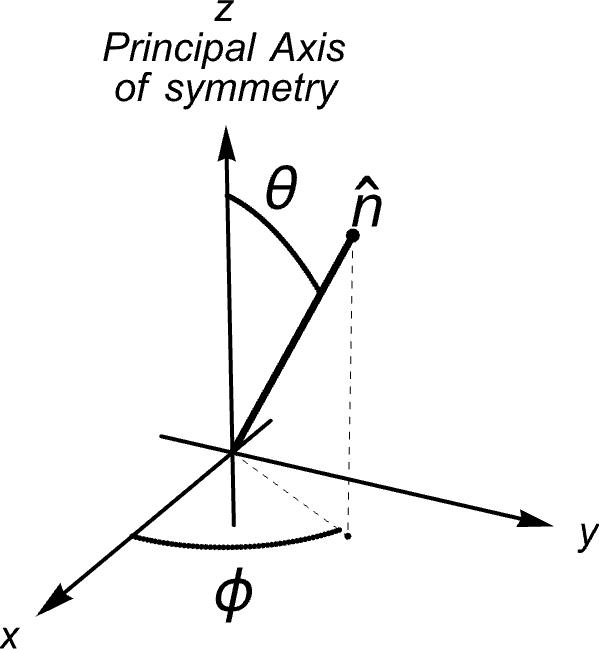
\includegraphics[width=0.35\textwidth]{./figures/coordSys.jpg}
	\label{fig:spherical-coord-sys} 
\end{figure}

\section{Spectroscopic measurements and uncertainty}\label{section:uncertainty}

We may categorize the uncertainty in the parameters fitted to experimental data in three categories: experimental, model, and others. 

Before listing the sources that contribute to experimental error, let's briefly recount the types of experiments that are used in order to determine level energies and state labels. The first type is absorption spectroscopy, in which a crystal, adequately doped, is illuminated with a broad spectrum light source, and the wavelength dependent absorption by the crystal thus determined. The crystals absorb radiation depending on the availability of a transition energy between the thermally populated low-lying states and excited levels. This data therefore provides transition energies between the ground multiplet and excited states. Furthermore, from this data one can also estimate the probability that a photon of a given wavelength is absorbed by the ions in the crystal, and from this one estimates the oscillator strength of a given transition. 

In order to inform to what two multiplets the transitions belong to, here one may already count how many lines arrange themselves in groups. Alas, this type of absorption spectroscopy is lacking in that it only provides information about transitions between the ground and excited states, and may even elide such transitions that are too weak to be observed. In view of this, some variety of emission spectroscopy becomes relevant. In these, the ions inside of the crystal are excited (thermally, electrically, or radiatively) and the light produced by the relaxing transitions are then registered. This has the benefit that one has now populated other states than the ground state (perhaps with aid of non-radiative transitions inside of the crystal or energy transfer) so that now one can also have information about transitions that depart from a state different than ground. From this type of spectroscopy,  given a transition, one may also determine its transition rate, given the availability of time-resolved emission; given this one may then give an upper bound on the spontaneous rate of identified transitions.

In these analyses a few things may not go according to plan:

\begin{enumerate}
	\item \textbf{Several non-equivalent symmetry sites}. Ions may not be located in sites with the same crystal symmetry. As such it will be problematic to interpret their crystal splittings based on the assumption of a single symmetry.
	\item \textbf{Non-homogeneous crystal field}. Even if they are located in sites with the same point symmetry, it may also be that the crystal field they experience has variations across the bulk of the crystal. As such, the observations would then rather be about an ensemble of crystal fields, instead of a single one.
	\item \textbf{Crystal impurities}. The doped crystals may contain impurities that will lead to the false identification of transitions to the ion of study. This may be disambiguated from pooling together several experiments.
	\item \textbf{Non-radiative transitions}, mediated by the crystal, will lead to shifts in transition energies, both in emission, and in absorption. This yields a confounding factor for the \textit{radiative} transition energies that are in principle required to be valid inputs to the model Hamiltonian. Comparison of emission and absorption lines is key to determine the relevance of this.
	\item \textbf{Spectrometer resolution}. The spectrometers used have a finite resolution. In the setups typically used for this, the nominal resolution might be of the order of $0.1\text{ nm}$.
	\item \textbf{Crystal transparency}. Observation of transitions within the ions requires that the crystal be mostly transparent at the relevant wavelengths.
\end{enumerate}

In the works of Carnall and others, the nominal uncertainty in the state energies is of $1 \Kayser$, this being the precision to which the used experimental energies are quoted.

With regards to model uncertainties, the following factors may be considered to contribute to it: 
\begin{enumerate}
\item \textbf{Intra-configuration transitions}. When energy levels reach a certain threshold, observations may no longer be intra-configuration transitions, but rather inter-configuration transitions. These transitions should not be included, so care must be taken to exclude them from the analysis.
\item \textbf{Unaccounted configuration interaction}. The model makes an attempt at describing configuration interaction effects, but this is only carried to second order in the types of considered interactions, and not all interactions are considered.
\end{enumerate}

Finally, in the ``others'' category we have the two following:

\begin{enumerate}
\item \textbf{Numerical precision.} No longer relevant with modern computers, however, at the time at which some of these calculations were done, numerical precision might account for some of the discrepancies one finds when comparing current calculations to old ones.
\item \textbf{Errors in tables with reduced matrix elements}. The Crosswhite group at Argonne National Lab produced a set of tables with the reduced matrix elements of operators. However, at some point, these tables became slightly corrupted, and subsequent codes that used them carried those errors with them. In \qlanth this problem is avoided since all reduced matrix elements are calculated from scratch.
\end{enumerate}

When the model parameters are fitted to experimental data and their uncertainties are being estimated, \qlanth offers two approaches. In the first approach a given constant uncertainty in the energy levels is assumed, this in turns determines the relevant contour of $\chi^2$, and from this the uncertainties in the model parameters are calculated.

In an alternative approach, the uncertainties are determined \textit{a posteriori}. The model parameters are fit to minimize the square differences between calculated energies and the experimental ones. Then, a single experimental uncertainty is assumed in all the energy levels, and taken equal to the minimum root mean  square error, as taken over the available degrees of freedom. This uncertainty $\sigma$ together with a chosen confidence interval $p$ is then used to determine the contours of $\chi^2$, which in turn determine the corresponding confidence interval in the model parameters. In a sense, the model is assumed to be valid, and the resulting uncertainties in the model parameters are adjusted to allow for this possibility.

In the examples included in this code the uncertainty in the experimental data was assumed to be constant and equal to $1 \invcm$. And when the data for magnetic dipole transitions was calculated, an uncertainty equal to the $\sigma$ of the related parametric fit was assumed. 

\section{Transitions}\label{section:transitions}

\qlanth can also compute magnetic dipole transition rates within states and levels, as well as forced electric dipole transition rates between levels.

\subsection{State description}

\subsubsection{Magnetic dipole transitions}

\qlanth can also calculate a few quantities related to magnetic dipole transitions. With $\op{\mu} = \{\op{\mu}_x, \op{\mu}_y, \op{\mu}_z\}$ the magnetic dipole operator, the line strength between two eigenstates $\ket{\nu}$ and $\ket{\nu'}$ is defined as (see for example equation 14.31 in \cite{cowan_theory_1981})
\begin{equation}
	\lineStrength(\psi,\psi') \DEF \left| \braopket{\psi}{\op{\mu}}{\psi'} \right|^2 = \left| \braopket{\psi}{\op{\mu}_x}{\psi'} \right|^2 + \left| \braopket{\psi}{\op{\mu}_y}{\psi'} \right|^2 + \left| \braopket{\psi}{\op{\mu}_z}{\psi'} \right|^2
\end{equation}

In \qlanth this is computed with the function \codetext{MagDipLineStrength}, which given a set of eigenvectors computes the sum above, and returns an array that contains all possible pairings of $\ket{\psi}$ and $\ket{\psi'}$ in $\lineStrength(\psi,\psi')$.
 
\lstinputlisting[language=Mathematica]{./fundefs/MagDipLineStrength.tex}

Using the line strength $\lineStrength$, the transition rate $\AMD$ for the spontaneous transition $\ket{\psi_i} \rightsquigarrow \ket{\psi_f}$ is then given by (from table 7.3 of \cite{thorne_spectrophysics_1999})
\begin{equation}
	\tRate{MD}{\psi_i}{\psi_f} = \frac{16 \pi^3 \mu_0}{3 h} \frac{n^3}{\lambda_{if}^3} \frac{\lineStrength(\psi_i,\psi_f)}{g_i},
\end{equation}
where $\lambda$ is the vacuum-equivalent wavelength of the transition between $\ket{\nu}$ and $\ket{\nu'}$, $n$ the refractive index of the medium containing the ion, and $g_i$ the degeneracy of the initial state $\ket{\psi_i}$. At the state level of description, $J$ is no longer a good quantum number so the degeneracy $g_i=1$. 

\lstinputlisting[language=Mathematica]{./fundefs/MagDipoleRates} 
 
A final quantity of interest is the oscillator strength for the transition between the ground state $\ket{\psi_g}$ and an excited state $\ket{\psi_e}$. The oscillator strength is a dimensionless quantity which is indicative of how strong absorption is. The oscillator strength may be defined for other initial states than the ground state, but since this is the state most likely to be populated in ordinary experimental conditions, this is the initial state that is of most frequent interest. The oscillator strength is given by \cite{carnall_spectral_1965}
\begin{equation}
	\oStrength{MD}{\psi_g}{\psi_e} = \frac{8 \pi^2 \me}{3\,hc\,e^2} 
	\frac{n}{\lambda_{ge}}
	\frac{\lineStrength(\psi_g,\psi_e)}{g_g}
\end{equation}
where $g_g$ is the degeneracy of the ground state. At the level of detail that the eigenstates are described in \qlanth where $J$ is no longer a good quantum number, $g_g = 1$. 

In \qlanth the function \codetext{GroundMagDipoleOscillatorStrength} implements the calculation of the oscillator strengths from the ground state to all the excited ones.

\lstinputlisting[language=Mathematica]{./fundefs/GroundMagDipoleOscillatorStrength} 

\subsection{Level description}

\subsubsection{Forced electric dipole transitions}

\index{forced electric dipole transitions}
Any two eigenfunctions that are approximated within the limits of a single configuration cannot help but have the same parity as they are spanned by basis vectors with definite and shared parity. Analysis of the amplitudes for different transition operators can then inform as to what transitions are forbidden, which are those in which the product of the parity of the two participating wavefunctions and that of the transition operator results in odd parity. As such, within the single configuration approximation, since the product of the two participating wavefunctions is always even, then any transition described by an operator of odd parity is forbidden. This is the content of \index{Laporte's rule} Laporte's parity selection rule. Since the parity of the magnetic dipole operator is even \footnote{The parity of the electric quadrupole operator is also even, but we haven't included it in \qlanth}, then this operator allows for  intra-configuration transitions, and since the parity of the electric dipole operator is odd, then these types of intra-configuration transitions are forbidden.

However, much as configuration interaction is an essential component in the description of the electronic structure, it has a bearing on the energy spectrum and the intra-configuration wavefunctions themselves. Configuration interaction may also be used to bring back into the analysis the fact that the \textit{actual} wavefunctions will also have at least a small part of them in other configurations, even if most of them may be within the ground configuration. It is therefore the case that the \textit{actual} parity of the wavefunctions is mixed, and therefore intra-configuration  \footnote{Calling these \textit{intra}-configuration transitions is somewhat of a misnomer since their nature is tied to the fact that the single-configuration description is wanting.} electric dipole transitions are actually allowed. These electric dipole transitions are called \textit{forced} electric dipole transitions.


\index{Judd-Ofelt theory}
Judd \cite{judd_optical_1962} and Ofelt \cite{ofelt_intensities_1962} came separately to similar versions of this analysis, and showed after a series of approximations that the forced electric dipole transitions could be described by the intra-configuration matrix elements of the multi-electron unit operators $\op{U}^{(k)}$ (for k=2,4,6) together with a set of three accompanying coefficients $\{\JOk{2},\JOk{4},\JOk{6}\}$. These coefficients have a definite form related to the overlap between the mixed parity parts of the corrected wavefunctions, but they can also be considered as additional phenomenological parameters.

Judd-Ofelt theory is based on the level description, and its mathematical expression is the following. Given two intermediate coupling levels $\ket{\alpha SLJ}$ and $\ket{\alpha\mathrlap{'} SL\mathrlap{'}J\mathrlap{'}\,}$, the oscillator strength between them is approximated as \cite{judd_optical_1962} 
\begin{equation}
\oStrength{f-ED}{\alpha{LSJ}}{\alpha\mathrlap{'} S\mathrlap{'} L\mathrlap{'} J\mathrlap{'}\,\,} = 
	\mathcal{R} \frac{8 \pi^2 m_e}{3 h}
	\frac{\nu}{\tpo{J}}
	\frac{\chi}{n} 
	\sum_{k=2,4,6}
		\JOk{k} 
		\left|
			\redbraopket{\forb^\numE \alpha SLJ}
				{\op{U}^{(k)}}
				{\forb^\numE \alpha\mathrlap{'} S\mathrlap{'} L\mathrlap{'} J'} 
		\right|^2,
\label{eqn:forced-dipole-judd-ofelt}
\end{equation}
where $\nu$ is the frequency of the transition, $\chi$ the local field correction, $n$ the refractive index of the crystal host, and $\mathcal{R} = 1$ in the case of absorption and $\mathcal{R} = n^2$ in the case of emission. 

The local field correction $\chi$ accounts for the difference between the macroscopic and microscopic electric fields, in the case of ions embedded for crystals the most common choice is 
\begin{equation}
	\chi = \frac{n^2+2}{3}  
\end{equation}
and for other environments (or emitters other than ions such as molecules) different alternatives are relevant (see \cite{duan_dependence_2006}).

In \qlanth Judd-Ofelt theory is implemented with help of the functions \codetext{JuddOfeltUkSquared} and \codetext{LevelElecDipoleOscillatorStrength}.

\lstinputlisting[language=Mathematica]{./fundefs/JuddOfeltUkSquared} 

\lstinputlisting[language=Mathematica]{./fundefs/LevelElecDipoleOscillatorStrength} 

\subsubsection{Magnetic dipole transitions}

In Hartree atomic units, the magnetic dipole line strength between levels $\ket{\alpha{LSJ}}$ and $\ket{\alpha\mathrlap{'} S\mathrlap{'} L\mathrlap{'} J\mathrlap{'}\,\,}$ is given by
\begin{equation} 
	\lineStrength(\ket{\alpha{LSJ}},\ket{\alpha\mathrlap{'} S\mathrlap{'} L\mathrlap{'} J\mathrlap{'}\,\,}) = 
	\left|\redbraopket{\alpha{LSJ}}{\frac{1}{2}(\op{L}+g \op{S})}{\alpha\mathrlap{'} S\mathrlap{'} L\mathrlap{'} J\mathrlap{'}\,\,} \right|^2
\end{equation}

In \qlanth the line strength can be calculated using the function \codetext{LevelMagDipoleLineStrength}.

\lstinputlisting[language=Mathematica]{./fundefs/LevelMagDipoleLineStrength} 

In atomic units, the magnetic dipole oscillator strength for a transition between level $\ket{\alpha{LSJ}}$ and an excited level $\ket{\alpha\mathrlap{'} S\mathrlap{'} L\mathrlap{'} J\mathrlap{'}\,\,}$ is given by \cite{rudzikas_theoretical_2007}
\begin{equation} 
	\oStrength{MD}{\alpha{LSJ}}{\alpha\mathrlap{'} S\mathrlap{'} L\mathrlap{'} J\mathrlap{'}\,\,} = \frac{2 n}{3}
	\frac{
	\mathcal{E}(
		\ket{\alpha\mathrlap{'}
			S\mathrlap{'}
			L\mathrlap{'}
			J\mathrlap{'}\,\,})-
	\mathcal{E}(
		\ket{\alpha{LSJ}
		)}}
	{2J+1}
	\alphaFine^2
	\lineStrength\left(\ket{\alpha{LSJ}},\ket{\alpha\mathrlap{'} S\mathrlap{'} L\mathrlap{'} J\mathrlap{'}\,\,}\right)
\end{equation}
where $\mathcal{E}(\ket{\alpha{LSJ}})$ is the energy of level $\ket{\alpha{LSJ}}$, $n$ is the refractive index of the medium, and $\alphaFine$ is the fine structure constant. In obtaining this expression one considers the transition from one state of the initial level into another single state of the final level. Furthermore, here it is assumed that all the states of the initial level are equally populated.

In \qlanth the function \codetext{LevelMagDipoleOscillatorStrength} can be used to calculate these.

\lstinputlisting[language=Mathematica]{./fundefs/LevelMagDipoleOscillatorStrength} 


A final quantity of interest is the spontaneous magnetic dipole decay rate from one level to a lower lying one. In atomic units this rate is determined by 
\begin{equation}
	\decayRate{MD}{\alpha{LSJ}}{\alpha\mathrlap{'}
			S\mathrlap{'}
			L\mathrlap{'}
			J\mathrlap{'}} = \frac{4 n^3}{3} 
			\frac{
				\left(
					\mathcal{E}(
						\ket{\alpha{LSJ}}) - 
					\mathcal{E}(
						\ket{\alpha\mathrlap{'}
							S\mathrlap{'}
							L\mathrlap{'}
							J\mathrlap{'}\,\,})
				\right)^3
				}
				{2J+1} 
		\alphaFine^5
		\lineStrength\left(\ket{\alpha{LSJ}},\ket{\alpha\mathrlap{'} S\mathrlap{'} L\mathrlap{'} J\mathrlap{'}\,\,}\right).
\end{equation}

In \qlanth the spontaneous decay rates may be calculated through the function \codetext{LevelMagDipoleSpotaneousDecayRates}.

\lstinputlisting[language=Mathematica]{./fundefs/LevelMagDipoleSpotaneousDecayRates} 

\section{Parameter constraints}\label{section:param-constraints}

When there is a scarcity of experimental data, one useful strategy to reduce the number of free parameters is to enforce some constraints between ratios of Slater integrals $\Fk{k}$, Marvin integrals $\Mk{k}$, and pseudo-magnetic parameters $\Pk{k}$.

 For the Slater integrals one may leave only $\Fk{2}$ as free parameter, and fix the ratios $\Fk{4}/\Fk{2}$ and $\Fk{6}/\Fk{2}$.
 
 For the Marvin integrals one often leaves only a single free parameter $\Mk{0}$, and give values to $\Mk{2}$ and $\Mk{4}$, by fixing the ratios $\Mk{2}/\Mk{0}$ and $\Mk{4}/\Mk{0}$.
 
 For the pseudo-magnetic parameters again the common practice is to only leave a single free parameter $\Pk{2}$, and give values to $\Pk{4}$ and $\Pk{6}$, by fixing the ratios $\Pk{4}/\Pk{2}$ and $\Pk{6}/\Pk{2}$.
 
 The values for all these ratios were historically obtained by using the integral expressions for the corresponding parameters, and calculating them using Hartree-Fock solutions to the radial parts of the wavefunctions. Examples of these ratios can be seen in the sections with data for \LaFthree and \liyorite.

\section{Fitting experimental data}\label{section:data-fitting}

\qlanth also has the capacity to fit the \hamilton to experimental data. This is included in the sub-module \codetext{fittings.m} (see \appendixref{sub:fittings.m}). This sub-module includes the function \codetext{ClassicalFit} which uses a truncated Hamiltonian (based on free-ion energies) to fit a given subset of the model parameters to given experimental data. It yields an extensive set of results, including fitted parameters and uncertainties. If the truncation energy parameter is set to infinity, then the fitting is performed with no truncation.  

\label{note:param-model}

This function, however, is specifically used for fitting data for a single ion in a specific host. In the case of fitting data for several ions, it may be necessary to use parameter trends $\Param(\numE)$. This is necessary since not only there might be some ions where there is no data (and where one would then propose a ``synthetic'' solution), but also since there are cases where there are too few data points to justify varying all of the model parameters.\footnote{The extreme case of this scarcity being Yb and Ce, where there are only 7 non-degenerate energies, but where the crystal-field alone might require more parameters than these (for instance in $C_{2v}$ symmetry one needs 9 $\Bkq{k}{q}$ parameters).}

In these cases where one is fitting data for all or most of the lanthanide ions in a given host, it is  useful to first fit the model in cases where there are the most data points, and to  build up a parameter model $\Param(\numE)$ for each parameter as the fitting of all the ions progresses. One feature often used in fitting for several ions (see \bill and \cheng) is that when there is scarcity of data (as mentioned above), one can then use the trends in the $\Param(\numE)$ in order to fix some parameter values at a given column (and proceed to vary others to fit the data to the model).\footnote{For example, in the \tableref{table:LaF3-qlanth-params} for \LaFthree, in the case of Yb, only two parameters are varied ($\zeta$ and $\epsilon$) and the values for the crystal field obtained from linear fits to the previously fitted $\Bkq{k}{q}$ in Pr, Nd, Dy,  Sm*, Ho*, Er, and Tm. (* not all $\Bkq{k}{q}$)}

Here below is a detailed explanation of the parameters required by \codetext{ClassicalFit}. The code for this function \codetext{ClassicalFit} may be found in \appendixref{sub:fittings.m}.

\begin{itemize}
	\item \codetext{numE}: number of electrons in the system, specifying the electronic configuration.

	\item \codetext{expData}: experimental data, a list of lists where each sublist represents an energy level and associated parameters. The first element of the sublists must represent energies, the other elements in the sublists are ignored but can be given to be kept together with the fitted data. The data must be ordered in increasing order of energy. \textbf{IMPORTANT:} if there are known unknown levels, these should be made explicit, anything other than a number will be interpreted as a level of undetermined energy in the corresponding gap. \textbf{ALSO IMPORTANT:} in the case of odd electron cases, \codetext{expData} needs to explicitly include the duplicate energies corresponding to Kramers' degeneracy; the gaps also need to be adequately duplicated in these cases.  

	\item \codetext{excludeDataIndices}: indices in \codetext{expData} to be excluded from the fitting process. This can be used to exclude experimental data which is present, but which is considered dubious. In the case of odd electron configurations, these indices need to explicitly include the double degeneracy of Kramers doublets.

	\item \codetext{problemVars}: symbols representing the parameters to be fitted, some of which may be constrained (set fixed or proportional to others). \textbf{IMPORTANT:} if \codetext{problemVars} is a proper subset of all the parameters needed to evaluate the simplified Hamiltonian, the values for the other necessary parameters are taken from the \bill systematic study of \LaFthree.

	\item \codetext{startValues}: an association with the initial values for the independent parameters given in \codetext{problemVars}. Independent parameters are those that remain once the constraints have been accounted for.

	\item \codetext{$\sigma$exp}: estimated uncertainty in the energy level differences between experimental and calculated values.

	\item \codetext{constraints}: a list of replacement rules defining constraints on the parameters. These constraints can either pin down a value, or apply proportionality ratios between them. If constrained by proportionally factors, these ratios are usually taken from Hartree-Fock calculations.
\end{itemize}

Here is a description of the different steps that this algorithm implements.
\begin{enumerate}
  \item \textbf{Initialization}: sets initial conditions, processes options, and prepares data structures. Manages settings like the truncation energy, logging preferences, and computational accuracy goals.
  
  \item \textbf{Data Preparation}: determines valid data points, excluding specified indices, and establishes truncation energy for the model.
  
  \item \textbf{Hamiltonian Assembly and Simplification}: constructs the Hamiltonian while preserving its block structure, applies simplification rules, and processes the diagonal blocks to retain only free-ion parameters.
  
  \item \textbf{Level Calculation}: determines the level description using free-ion parameters.
  
  \item \textbf{Compilation and Truncation of Hamiltonian}: compiles the Hamiltonian and truncates it based on the set truncation energy, optimizing for computational efficiency.
  
  \item \textbf{Fitting Process Initialization}: prepares variables and functions for optimization, including eigenvalue calculations and difference evaluations.
  
  \item \textbf{Optimization}: employs the Levenberg-Marquardt method to optimize parameters, minimizing the discrepancy between calculated and experimental energy levels.
  
  \item \textbf{Post-Processing}: calculates the Hamiltonian's eigensystem at the solution, deriving statistics like RMS deviation, parameter uncertainties, and covariance matrix.
  
  \item \textbf{Output Compilation}: aggregates all relevant data and results into the output association \codetext{solCompendium}, documenting the fitting process and outcomes.
  
  \item \textbf{Logging and Return}: saves the comprehensive fitting results to a log file and returns the detailed output data.
\end{enumerate}

This function admits several options. Importantly here one may permit the model to have a constant shift to all the levels and the truncation energy can be set. Here one can also provide simplification rules that are applied to the compiled version of the Hamiltonian.

\begin{itemize}

	\item \codetext{Energy Uncertainty in K}: used for error estimation, it can be either \codetext{Automatic} in which case the ($\sigma$ of the fit is used as the uncertainty of the energies) or a numeric value in which case that is the value used for error propagation.

	\item \codetext{TruncationEnergy}: determines the energy level at which the Hamiltonian is truncated. If set to \codetext{Automatic}, the truncation energy is derived from the maximum energy present in the experimental data (\codetext{expData}). Otherwise, it can be manually set to a specific value.
	
	\item \codetext{MagneticSimplifier}: provides a list of replacement rules to simplify the magnetic parameters in the Hamiltonian, aiding in the reduction of computational complexity.
	
	\item \codetext{MagFieldSimplifier}: offers a list of replacement rules to specify a magnetic field, enhancing the flexibility in modeling magnetic effects within the system.
	
	\item \codetext{SymmetrySimplifier}: A list of replacement rules used to simplify the crystal field components of the Hamiltonian, facilitating a more efficient fitting process.
	
	\item \codetext{OtherSimplifier}: an additional list of replacement rules applied to the Hamiltonian before computation, allowing for further customization and simplification of the model, such as disabling specific interactions or effects. \textbf{IMPORTANT}: here the default is that the spin-spin contribution (as controlled by the $\sigma$SS parameter) for the Marvin integrals is \textit{not} included.
	
	\item \codetext{MaxHistory}: this option controls the length of the logs for the solver, enabling users to adjust the amount of log data retained during the fitting process.
	
	\item \codetext{MaxIterations}: sets the maximum number of iterations that the fitting algorithm (\codetext{NMinimize}) will execute, allowing control over the computational effort spent on the fitting.
	
	\item \codetext{FilePrefix}: specifies the prefix for the filenames under which the fitting results are saved. By default, the prefix is set to ``calcs'', and the files are saved in the ``log/calcs'' directory.
	
	\item \codetext{AddConstantShift}: if set to \codetext{True}, this option allows for a constant shift in the energy levels during the fitting process. This is particularly useful for fine-tuning the model to better match experimental data.
	
	\item \codetext{AccuracyGoal}: defines the accuracy goal for the \codetext{NMinimize} function used in the fitting process, allowing users to set the desired level of precision for the fit.
	
	\item \codetext{PrintFun}: specifies the function used to print progress messages during the fitting process. The default is \codetext{PrintTemporary}, which displays temporary output that can be useful for monitoring the fitting's progress.
	
	\item \codetext{SlackChannel}: names the Slack channel to which progress messages will be sent. If set to \codetext{None}, this feature is disabled, and no messages are sent to Slack.
	
	\item \codetext{ProgressView}: controls whether a progress window is displayed during the fitting process. When set to \codetext{True}, it provides an auxiliary notebook is created automatically with plots showing the progress of \codetext{NMinimize}.
	
	\item \codetext{SignatureCheck}: if \codetext{True}, the function ends prematurely and prints the  list of the symbols that define the Hamiltonian after all basic simplifications have been applied without considering the given constraints.
	
	\item \codetext{SaveEigenvectors}: determines whether both the eigenvectors and eigenvalues of the fitted model are saved. If set to \codetext{False}, only the energies are saved.
	
	\item \codetext{AppendToLogFile}: what is provided here is appended to the log file under the ``Appendix'' key, enabling additional data to be stored alongside the fitting results.
\end{itemize}

The function returns an association with the following keys.

\begin{itemize}
    \item \codetext{bestRMS}: the best root mean square deviation found during the fitting process.

    \item \codetext{bestParams}: the optimal set of parameters found through the fitting process.

    \item \codetext{paramSols}: a list of the parameter solutions at each step of the fitting algorithm.

    \item \codetext{timeTaken/s}: the total time taken to complete the fitting process, measured in seconds.

    \item \codetext{simplifier}: the replacement rules used to reduce the define the free-ion Hamiltonian.

    \item \codetext{excludeDataIndices}: the indices that were excluded from the fitting process as specified in the input.

    \item \codetext{startValues}: the initial values for the problem variables as given in the input.

    \item \codetext{freeIonSymbols}: symbols used in the intermediate coupling level calculation.

    \item \codetext{truncationEnergy}: the energy level at which the Hamiltonian was truncated.

    \item \codetext{numE}: the number of electrons in the $f^{\text{numE}}$ configuration.

    \item \codetext{expData}: the experimental data used for the fitting process. 

    \item \codetext{problemVars}: the variables considered during the fitting process.

    \item \codetext{maxIterations}: the maximum number of iterations used in the fitting process.

    \item \codetext{hamDim}: the dimension of the full Hamiltonian before simplifications or truncations.

    \item \codetext{allVars}: all the symbols defining the Hamiltonian under the applied simplifications.

    \item \codetext{freeBies}: the free-ion parameters used to calculate the intermediate coupling levels.

    \item \codetext{truncatedDim}: the dimension of the truncated Hamiltonian.

    \item \codetext{compiledIntermediateFname}: the file name of the compiled function used for the truncated Hamiltonian.
 
    \item \codetext{fittedLevels}: the number of levels that were fitted.

    \item \codetext{actualSteps}: the actual number of steps taken by the fitting algorithm.

    \item \codetext{solWithUncertainty}: a list of replacement rules showing the best fit value and its uncertainty for each parameter.

    \item \codetext{rmsHistory}: as list of the RMS values found during the fitting process.

    \item \codetext{Appendix}: an association appended to the log file under the ``Appendix'' key.

    \item \codetext{presentDataIndices}: the indices in \codetext{expData} that were used for fitting.

    \item \codetext{states}: a list of eigenvalues and eigenvectors for the fitted model, available if eigenvectors were saved.

    \item \codetext{energies}: a list of the energies of the fitted levels, adjusted if an energy shift was included in the fitting.
\end{itemize}

\foreach \name in {ClassicalFit}{
    \lstinputlisting[language=Mathematica]{./fundefs/\name.tex}
}

\section{Accompanying notebooks}\label{section:notebooks}

The code for this dissertation is accompanied by the following auxiliary \mathematica notebooks, which either document the  functions included in the code, or serve as aids in the  calculation of matrix elements. These notebooks assume that the \codetext{paclet} has been installed according to the instructions given in \sectionref{section:paclet}.

\begin{itemize}
%	\item \faFloppyO\,\, \codetext{/notebooks/qlanth.nb}: gives an overview of functions included in \qlanth.
	\item \faFloppyO\,\, \codetext{/notebooks/qlanth - Table Generator.nb}: generates the basic tables on which every calculation is based. This means that LS-reduced matrix elements are used to calculate matrix elements in the $\LSJMbasis$ basis.
	\item \faFloppyO\,\, \codetext{/notebooks/qlanth - JJBlock Calculator.nb}: can be used to generate the J-J' blocks for the different interactions. The data files produced here are necessary for \codetext{HamMatrixAssembly} to work. These blocks are creating by putting together matrix elements from different interactions.
	\item \faFloppyO\,\, \codetext{/notebooks/The Lanthanides in LaF3.nb}: runs \qlanth over the lanthanide ions in \LaFthree and compares the results against the published values from \bill. It also calculates magnetic dipole transition rates and oscillator strengths.
\end{itemize}

\section{Compiled data for \LaFthree:$\trion{Ln}$ and \liyorite:$\trion{Ln}$}\label{section:data}

The study of \bill on lanthanum fluoride was a systematic review of trivalent lanthanide ions in \LaFthree. In this work they fitted the experimental data for all of the lanthanide ions using the single-configuration effective Hamiltonian. In their appendices one can find their calculated values, together with the experimental values that they used for their least squares fittings. In \qlanth this data can be accessed by invoking the command \codetext{LoadCarnall} which brings into the session an association that has keys that have as values the tables and appendices from this article. \figuref{fig:dieke-laf3} shows the results of a calculation done with \qlanth for the energy levels in \LaFthree. Additionally the function \codetext{LoadLaF3Parameters} can be used to query the data for the fitted parameters, which may serve as a useful starting point for the description of the lanthanides ions in hosts other than \LaFthree.

\begin{figure}[h!]
	\centering
	\includegraphics[width=0.9\textwidth]{./figures/DiekePlot-LaF3.pdf}
	\caption{Energy levels in \LaFthree.}	
	\label{fig:dieke-laf3}
\end{figure}


Similarly, \cheng compiled data for \liyorite. In \qlanth model parameters for \liyorite can be obtained by calling the function \codetext{LoadLiYF4Parameters}. \figuref{fig:dieke-liyf4} shows the results of a calculation done with \qlanth for the energy levels in \liyorite. 

\begin{figure}[h!]
	\centering
	\includegraphics[width=0.9\textwidth]{./figures/DiekePlot-LiYF4.pdf}
	\caption{Energy levels in \liyorite.}	
	\label{fig:dieke-liyf4}
\end{figure}


\foreach \name in {Carnall, LoadCarnall, LoadLaF3Parameters, LoadLiYF4Parameters}{
    \lstinputlisting[language=Mathematica]{./fundefs/\name.tex}
}



\section{\codetext{sparsefn.py}}\label{section:sparsefn}

	\qlanth is also accompanied by seven Python scripts \codetext{sparsef[1-7].py}. Each of these contains a function \codetext{effective\_hamiltonian\_f[1-7]} which returns a sparse array (using this data structure as provided by \codetext{scipy}) for given values for the model parameters.
	
	There is an eight Python script called \codetext{basisLSJMJ.py} which contains a dictionary whose keys are f1, f2, f3, f4, f5, f6, and f7, and whose values are lists that contain the ordered basis in which the array produced by the \codetext{sparsefn.py} should be understood to be in. Each basis vector is a list with three elements \{LS string in NK notation, $J$, $\Msub{J}$\}.

	In those it is left up to the user to make the adequate change of signs in the parameters for configurations above $\forb^7$.  These include changing the signs of all in \eqnref{eqn:flipped} and setting \codetext{t2Switch} to 0. For configurations at or below $\forb^7$ it is necessary to set \codetext{t2Switch} to 1.

\section{Data sources}\label{section:data-sources}

	The data (and their provenance) upon which \qlanth bases its calculations is the following:
	
	\begin{itemize} 
		\item Coefficients of fractional parentage and seniority numbers from Velkov \cite{velkov_multi-electron_2000}.
		\item Terms labels from $\forb^1$ to $\forb^7$ from Nielson and Koster \cite{nielson_spectroscopic_1963}.
		\item 3j-symbol \cite{wolfram_research_threejsymbol_2024} and 6j-symbol \cite{wolfram_research_sixjsymbol_2024} values from \mathematica (v 13.2),
		\item Reduced matrix elements for the three body operators from Judd \cite{judd_complete_1984}.
		\item Reduced matrix elements for the magnetic interactions from Judd \cite{judd_intra-atomic_1968}. 
	\end{itemize}

\section{Other details}\label{section:other-details}

	\begin{itemize}
		\item Fitting the experimental data for the entire row might take about 45 minutes, if run for the first time, but takes much less time once compiled functions from the truncated (or not truncated) Hamiltonian have been saved to disk.
		\item The code was run in \mathematica version 14.1 on MacOS Sequoia 15.2.
	\end{itemize}


\section{Units}\label{section:units}

Following the tradition of the spectroscopic community, all the matrix elements of the Hamiltonian are calculated using the Kayser ($\Kayser \equiv \text{cm}^{-1}$) as the (pseudo) energy unit. All the parameters (except the magnetic field which is in Tesla) in the effective Hamiltonian are assumed to be in this unit. As is customary, the angular momentum operators assume atomic units in which $\hbar=1$.

Some constants and conversion values are included in the file \codetext{qonstants.m}.

\lstinputlisting[language=Mathematica]{../Kernel/qonstants.m}

\section{Notation}\label{section:notation}

\begin{gather}
    \overbracket{\,\,\,\,\,\op{l}\,\,\,\,\,}^{\text{orbital angular momentum operator of a single electron}} \\
    \overbracket{\,\,\op{L}\,\,}^{\text{total orbital angular momentum  operator}} \\
    \overbracket{\,\,\op{s}\,\,}^{\text{spin angular momentum  operator of a single electron}} \\
    \overbracket{\,\,\op{S}\,\,}^{\text{total spin angular momentum operator}} \\
    \overbracket{\,\,\Lambda\,\,}^{\text{Shorthand for all other quantum numbers}} \\ 
    \overbracket{\,\,\lorb\,\,}^{\text{orbital angular momentum number}} \\
    \overbracket{\,\,\sspin\,\,}^{\text{spinning angular momentum number}} \\
    \overbracket{\,\,\CoulombNonCentral\,\,}^{\text{Coulomb non-central potential}} \\
    \overbracket{\redbraopket{\Lambda LS}{\op{O}}{\Lambda' L'S'}}^{\text{LS-reduced matrix element of operator }\hat{O}\text{ between }{\Lambda LS} \text{ and } {\Lambda' L'S'}} \\
    \overbracket{\redbraopket{\Lambda LSJ}{\op{O}}{\Lambda' L'S'J'}}^{\text{LSJ-reduced matrix element of operator }\hat{O}\text{ between }{\Lambda LSJ} \text{ and } {\Lambda' L'S'J'}} \\
    \overbracket{\LSterm{2 S + 1}{$\alpha$L}\equiv \ket{\alpha{LS}}}^{\text{Spectroscopic term } {\alpha{LS}} \text{ in Russel-Saunders notation }} \\
    \overbracket{\op{X}^{(k)}}^{\text{spherical tensor operator of rank k}} \\
    \overbracket{\op{X}_q^{(k)}}^{\text{q-component of the spherical tensor operator }\op{X}^{(k)}} \\
    \overbracket{\cfp{\lorb^{n-1}\alpha'L'S'}{\lorb^n\alpha{L}{S}}}^{\text{The coefficient of fractional parentage from the parent term }\ket{\lorb^{n-1}\alpha'{L'S'}}\text{ for the daughter term }\ket{\lorb^{n}\alpha{LS}}}  
\end{gather}

\section{Mathematica \codetext{paclet}}\label{section:paclet}


The simplest way of adding \qlanth to \mathematica is by installing the corresponding paclet. After having cloned the repository to a local machine, execute the code below in a \mathematica session. After this, the downloaded files may be removed, and \qlanth may be loaded into a notebook by issuing the command \codetext{Needs["DavidLizarazo{\textasciigrave}qlanth{\textasciigrave}"]} .

\begin{verbatim}
Needs["PacletTools`"];
pathToRepo = "~/Downloads/qlanth/"; (* change accordingly *)
pathToBuild = FileNameJoin[{pathToRepo,"build","DavidLizarazo__qlanth"}];
CreatePacletArchive[pathToBuild];
pathToPaclet = FileNames[
	FileNameJoin[{pathToRepo, "build", "/*.paclet"}]][[1]];
PacletInstall[pathToPaclet, ForceVersionInstall -> True];
\end{verbatim}

The paclet includes documentation in standard \mathematica format (see \figuref{fig:mathematica-docs}).

\begin{figure}
	\centering
	\begin{subfigure}{0.45\textwidth}
        \centering
		\includegraphics[width=\linewidth]{./docImages/141-qlanth.jpg}	
		\caption{\qlanth guide in \mathematica}
		\label{fig:mathematica-docs}
    \end{subfigure}
	\begin{subfigure}{0.45\textwidth}
        \centering
		\includegraphics[width=\linewidth]{./docImages/81-HamMatrixAssembly.jpg}	
		\caption{Documentation for \codetext{HamMatrixAssembly}}
		\label{fig:mathematica-docs-hammatrix}
    \end{subfigure}
    
    \vspace{1cm} 
    
	\begin{subfigure}{0.45\textwidth}
        \centering
		\includegraphics[width=\linewidth]{./docImages/15-BasisLSJMJ.jpg}	
		\caption{Doc. for \codetext{BasisLSJMJ}}
		\label{fig:mathematica-docs-basislsjmj}
    \end{subfigure}
	\begin{subfigure}{0.45\textwidth}
        \centering
		\includegraphics[width=\linewidth]{./docImages/184-ToPythonSymPyExpression}	
		\caption{Doc. for \codetext{ToPythonSymPyExpression}}
		\label{fig:mathematica-docs2}
    \end{subfigure}
\end{figure}


\section{Definitions}\label{section:definitions} 

\begin{gather} 
    \overbracket{\tpobraket{x} \DEF 2x+1}^{\text{two plus one}} \\
    \overbracket{\op{u}^{(k)}}^{\text{irreducible unit tensor operator of rank k}} \\ 
    \overbracket{\op{U}^{(k)} \DEF \sum_{i=1}^{n} \op{u}^{(k)} }^{\text{symmetric unit tensor operator for n equivalent electrons}} \\
    \overbracket{\Ckq{k}{q} \DEF \sqrt{\frac{4\pi}{2k+1}} \Ykq}^{\text{Renormalized spherical harmonics}} \\
    \overbracket{\tricondition{j_1,j_2,j_3} \DEF
    \begin{cases} 
        1 & \text{if } j_1 = (j_2 + j_3), (j_2 + j_3 - 1), \ldots, |j_2-j_3|\\
        0 & \text{otherwise}
        \end{cases}}^{\text{Triangle ``delta'' between $j_1,j_2,j_3$}} 
\end{gather}

\newpage

\section{code}\label{section:code}

\subsection{qlanth.m}

This file encapsulates the main functions in \qlanth and contains all the physics related functions.

\lstinputlisting[language=Mathematica]{../Kernel/qlanth.m}

\subsection{fittings.m}\label{sub:fittings.m}

This file has code useful for fitting the Hamiltonian.

\lstinputlisting[language=Mathematica]{../Kernel/fittings.m}

\subsection{qplotter.m}\label{sub:qplotter.m}

This module has a few useful plotting routines.

\lstinputlisting[language=Mathematica]{../qplotter.m}

\subsection{misc.m}\label{sub.misc.m}

This module includes a few functions useful for data-handling.

\lstinputlisting[language=Mathematica]{../Kernel/misc.m}

\newpage

\printbibliography

\newpage

\printindex

%\newpage
%
%\thispagestyle{empty}
%
%\noindent
%%\hspace*{-\oddsidemargin} % Adjust this value if needed
%\makebox[\textwidth][c]{%
%    \includegraphics[width=5\textwidth]{./figures/pm_code.jpg}
%}

\end{document} 
